
\subsection{Batería de Litio-Ion}

La energía eléctrica ha empoderado a la sociedad desde su descubrimiento y,
gracias a los avances tecnológicos, el acceso a la misma se vuelve cada vez más
sencillo y más eficiente incluso en las ubicaciones más remotas del planeta.
Sumado a eso, nos dirigimos a una sociedad que se aprovecha cada vez más de la
movilidad eléctrica a medida que la dependencia de una conexi\'on local es
menor.

En gran parte, estos desarrollos son posibles gracias al descubrimiento del
litio-ion y su aplicacion en baterías. Este tipo de batería ha revolucionado la
tecnolog\'ia en almacenamiento de energ\'ia y ha logrado impulsar la
revoluci\'on digital empoderando los dispositivos móviles, a trav\'es de su gran
capacidad y densidad energ\'etica.

\subsubsection{Principios b\'asicos}

El principio básico de funcionamiento de una batería, en su configuraci\'on
b\'asica, consiste en una celda compuesta por dos electrodos 
\emph{(Fig. \ref{batt_wk_ppl})}, cada una conectada a un circuito el\'ectrico, 
separado por un electrolito que es capaz de acomodar cargas dentro de sí. 
Frecuentemente, los electrodos son f\'isicamente separados por una barrera que 
previene que estén en contacto físico entre ellos, evitando así un corto 
circuito en la batería. En descarga, cuando la bater\'ia entrega corriente al 
circuito, toma lugar un proceso de oxidación en el electrodo negativo (\'anodo), 
resultando en un movimiento de electrones a trav\'es del circuito. Por el otro 
lado, en el electrodo positivo (c\'atodo), ocurre un proceso de reducción, 
reabastecido por los electrones del circuito. El voltaje de la celda depende 
fuertemente de la diferencia de potencial entre los electrodos, y del proceso 
espont\'aneo en su totalidad. Para baterías recargables el proceso puede ser 
reversible aplicando electricidad externa produciendo un proceso complementario 
de \emph{redox} (reducci\'on-oxidac\'on) en los electrodos. Este proceso es 
dependiente de la energ\'ia y es no espont\'aneo, es decir, que sucederá s\'i y 
solo s\'i un agente externo participa en el proceso.

\noindent En base a este principio de funcionamiento, surgen una gran variedad
de tecnologías, partiendo de la pila voltaica, hecha de dos discos de metales
distintos, uno de zinc y otro de cobre o plata, separados por un dieléctrico
(como cartón o cuero) sumergido en una solución electrolítica. Durante la
operación, el disco de zinc actua como ánodo, liberando electrones al circuito y
produciendo iones de metal (proceso de oxidación), mientras que la reacción en
el electrodo opuesto depende de las condiciones de trabajo. En presencia del
aire, el metal de cobre es parcialmente oxidado a CuO, y la reducción de CuO a
Cu se da en el electrodo. En la ausencia de aire, los protones en el electrolito
son reducidos a hidrógeno en la superficie del cobre. El voltaje de la celda es
de aproximadamente 0.8-1.1V, dependiendo de la exposición al aire. 
Esencialmente, la pila voltaica es una batería no recargable.

\begin{figure}[h!]
    \begin{center}
	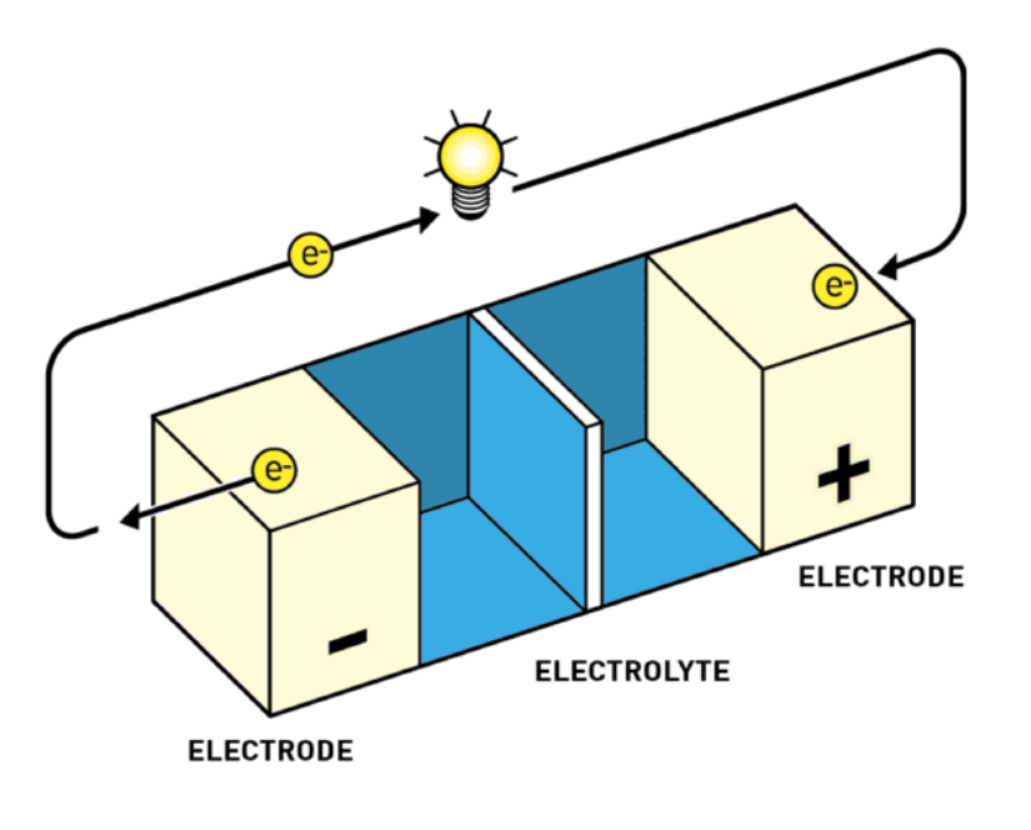
\includegraphics[width=0.4\textwidth]{batt_func_ppr.png}
    \end{center}
    \caption{Diagrama del principio básico de funcionamiento de una bater\'ia 
        en el proceso de descarga.}
    \label{batt_wk_ppl}
\end{figure}

\noindent Despu\'es surgieron las baterías de plomo-ácido, que su principio
de operaci\'on es similar a las baterías voltaicas expuestas al aire, pero con
la posibilidad de ser recargadas. Esta tecnología se basa en dos electrodos de
plomo, donde uno se encuentra parcialmente oxidado, en este caso es  oxido de 
plomo ($\mathrm{PbO_2}$), separado por \'acido sulf\'urico que contiene un 
electrolito. Durante el proceso de descarga, ocurre un proceso de oxidaci\'on 
en el electrodo de plomo (\'anodo), produciendo electrones, protones y sulfato 
de plomo ($\mathrm{PbSO_4}$), mientras que el \'oxido de plomo es reducido a
$\mathrm{PbSO_4}$ en el cátodo. En este caso, el potencial de una celda es de
alrededor 2V.

\noindent Otro logro en el desarrollo de baterías, ocurrió en el 1899 cuando se
desarrolló la primer batería de n\'iquel-hierro (Ni-Fe) y n\'iquel-cadmio
(Ni-Cd) o también conocidas como baterías alcalinas, que fueron predecedoras del
híbrido n\'iquel-metal (Ni-MH) que fue comercializada en 1898.

\noindent Las baterías anteriores son basadas en soluciones acuosas y la
densidad energética de las mismas no es alta, espec\'ificamente son menores a
los 100Wh/kg. Para incrementar la densidad energética de estas baterías, es
necesario encontrar una estabilidad electroquímica del agua ya que juega un rol
muy importante en ello. Además, es necesario buscar nuevos metales para
constituir los electrodos de las celdas ya que cuando \'ambos utilizan plomo,
debido al potencial del mismo, el voltaje de salida solo puede alcanzar un
máximo de 2.2V. Como resultado de los avances tecnol\'ogicos dentro del mercado
de consumo electr\'onico surge la necesidad de incrementar la densidad
energética de una celda, por lo tanto se impuls\'o la b\'usqueda de nuevas
tecnolog\'ias que permitan obtener una mayor capacidad en las bater\'ias con un
tamaño reducido, permitiendo el descubrimiento las propiedades del metal de
litio y su aplicacicación en las celdas que llevan su nombre.

\subsubsection{Litio}

El litio es un metal descubierto en 1818 que tiene excelentes propiedades para
servir como material para el desarrollo de baterías. Es el metal m\'as liviano
con una densidad de 0.53$\mathrm{g/cm^3}$. Tambi\'en tiene un potencial de
reducci\'on muy bajo, que lo hace ideal para celdas de alta densidad y alto
voltaje. Sin embargo, es un metal reactivo que debe ser protegido, por ejemplo,
del agua y del aire, ya que el contacto con estos provoca que el mismo sea muy
complicado de controlar, imposibilitando su uso para la aplicación deseada. Esta
protección al medio no es trivial, y factores, tales como su carácter inerte,
punto de fusión, la estabilidad del \emph{redox}, solubilidad de iones de litios
y sales, velocidades de transferencia ion/electrón, viscosidad, entre otros,
deben ser considerados.

\noindent Las primeras baterías de litio alcanzaron el mercado en 1970 y la
comercialización de las mismas comenzó en Japón en el año 1991, cuando
\emph{Sony Corporation} presentó el primer modelo.

\noindent Las baterías de litio-ion son definidas en \cite{Tatsuo2014} como
almacenadores de energía que utilizan iones de Litio como portadores de carga.
En base a esta definición, el término \emph{batería de Litio-Ion} no se
corresponde con una sola composición química, como lo son las baterías de ácido
o n'iquel-cadmio, si no que expresa una familia de baterías que dependen de los
iones de litio pero que pueden ser conformadas por distintos materiales.

%\newpage

\noindent A diferencia de las baterías de ácido, hay dos razones principales por
las cuales las baterías de litio-ion han crecido en popularidad en tan poco
tiempo: su excelente rendimiento y la capacidad de adaptarse al creciente
mercado de la electrónica de consumo, como por ejemplo, videograbadoras,
celulares y computadoras. A partir de la primer década del siglo XXI, se
comenzaron a utilizar en vehículos eléctricos, como también en grandes sistemas
de almacenamiento de energía, capaces de alimentar barrios residenciales
enteros.

\noindent Desde el 2000 al presente, se desarrollaron varios tipos de 
bater\'ias basadas en el litio. Entre ellas se encuentran las bater\'ias de 
litio-sulfuro (Li-S) y litio-aire (Li-air), cuya densidad energética teórica 
ronda los 2600Wh/kg y 11400 Wh/kg, respectivamente. En 2012, se desarrolló una 
batería de litio-ion recargable acuosa o \acrshort{ARLB} (del ingles
\emph{\acrlong{ARLB}}), que utiliza metal de litio recubierto como ánodo en una
solución de electrolitos mejorando ampliamente la densidad energética.

\subsubsection{Principio de funcionamiento}\label{battery_fun}

El principio de los procesos de carga y descarga en las baterías de litio-ion se
pueden describir utilizando como ejemplo el óxido de litio-cobalto 
($\mathrm{LiCoO_2}$) y grafito que son materiales de electrodo t\'ipicos en la
fabricaci\'on de las mismas. La Figura \ref{op_lithium-ion} ilustra el
princio de operación, y las reacciones de los electrodos se expresan en  las
Ecuaciones \ref{li_anode}, \ref{li_catode} y \ref{li_total}

\reaction{\text{Electrodo positivo: } LiCoO2 <=>[Carga][Descarga] Li_{1-x}CoO2 + xLi + xe^- \label{li_anode}}
\reaction{\text{Electrodo negativo: }6C + xLi^+ + xe^- <=>[Carga][Descarga] Li_{x}C6 \label{li_catode}}
\reaction{\text{Reaccion total: }6C + LiCoO2 <=>[Carga][Descarga] Li_{x}C6 + Li_{1-x}CoO2 \label{li_total}}

\noindent El \ce{LiCoO2} tiene una estructura reticular octa\'edrica con un
arreglo alternativo de capas de \ce{Li+} y \ce{Co^{3+}}. Durante el proceso de
carga, los iones de litio (en estado iónico) se desintercalan de la estructura
de capas del material del electrodo positivo, liberando electrones, al mismo
tiempo, el \ce{Co^{3+}} se oxida convirti\'endose en \ce{Co^{4+}}.  Por el otro
lado, durante el proceso de descarga, con la intercalación de \ce{Li+} dentro de
la ret\'icula, el \ce{Co^{4+}} es reducido a \ce{Co^{3+}}, ganando electrones,
adem\'as se obtienen electrones de la ret\'icula para convertirse en litio en 
estado atómico. Durante este proceso, el estado atómico del litio pierde 
electrones convirtiendose en iones de litio, este proceso se puede resumir en 
que el ánodo provee al electrodo positivo iones de litio. Dado que el litio se 
mueve entre el electrodo positivo y negativo hacia ambos lados a este tipo de 
baterías se las puede definir como una batería \emph{mecedora} (del ingles,
\emph{rocking chair}).

\begin{figure}[h!]
    \begin{center}
	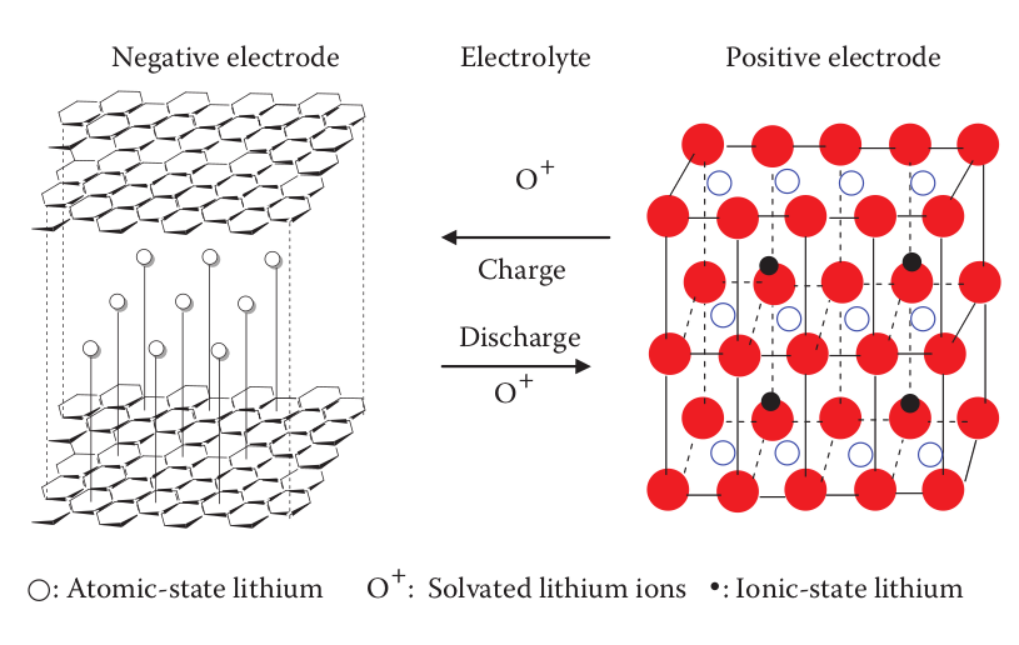
\includegraphics[width=0.7\textwidth]{prin_litio}
	\caption{Esquem\'atico del principio de operaci\'on de una bater\'ia de
	litio-ion.}
	\label{op_lithium-ion}
    \end{center}
\end{figure}

\noindent La mayoría de estas baterías usan materiales de carbón, tales como el
grafito o el carbón duro como ánodo. Otros utilizan óxidos de metales, como por
ejemplo, el titanato de litio ($\mathrm{Li_4Ti_5O_{12}}$) o el pentóxido de
niobio ($\mathrm{Nb_2O_5}$), debido a que pueden aceptar iones de litio cuando
son cargados, y liberarlos en el proceso de descarga, \'estas reacciones se
denominan como inserción y extracción respectivamente. Los potenciales de
reacción de estos materiales son mucho más bajos que los electrodos de hidrógeno
estándares, por lo tanto, el electrolito debería ser estable inclusive para
niveles de potencial tan bajos. Ésta es la razón por la cual, los electrolitos
orgánicos, que consisten de solventes orgánicos y sales de litio, son utilizados
en las baterías de Litio-ion en vez de electrolitos acuosos.

\noindent El material activo del cátodo debe contener Litio en su composición
química para proveer una fuente de iones de litio. Durante la primer etapa de
desarrollo de las celdas de litio, se utilizaba \'oxido de litio-cobalto.
También se estudió el uso de $\mathrm{LiNiO_2}$ (\'oxido de litio-nickel) como 
material activo para el cátodo pero fue inmediatamente descartado debido a su 
inestabilidad térmica. Sin embargo, se desarrollaron y utilizaron derivativos de 
esta composición, formulados como $\mathrm{LiM_xNi_{1-x}O_2}$  
(M: elemento metálico tales como, el cobalto, manganeso, aluminio o magnesio).

\newpage

\noindent Comparada con las baterías de litio-ion originales en los principios 
de 1990, el rendimiento de las mismas ha mejorado, de forma significativa, con 
el paso del tiempo. Los últimos desarrollos tienen ventajas dominantes sobre 
las baterías recargables tradicionales:

\begin{itemize}
    \item \textbf{Alta densidad energética:} La densidad energética por
	volumen y masa para una batería de litio modelo 18650 puede alcanzar
	los 500 Wh/$\mathrm{dm^3}$ y 230 Wh/kg, respectivamente, que adem\'as
	se encuentra en continuo aumento a medida que se investigan y
	desarrollan nuevas tecnologías.
    \item \textbf{Alto voltaje de salida (3.6V):} Esto es 3 veces 
        mayor a las baterías recargables de Ni-Cd o Ni-MH.
    \item \textbf{Alta potencia de salida:} Pueden alcanzar hasta 2kW/kg for
	un corto per\'iodo de tiempo.
    \item \textbf{Baja auto-descarga:} La descarga media de las celdas de
	litio son menores a un 3\% mensuales, que es la mitad que las celdas
	basadas en Ni-Cd y Ni-MH.
    \item \textbf{Bajo efecto de histéresis} A diferencia de las celdas de
	Ni-Cd y Ni-MH las celdas de litio tienen un efecto de histéresis
	despreciable con el paso de los ciclos de carga-descarga de la
	misma, resultando en un mejor ciclo de vida con respecto a los otros
	tipos de celdas.
    \item \textbf{Ciclos de carga-descarga rápidos:} Las baterías de
	litio-ion pueden ser cargadas con corrientes de hasta un 80\% de su
	capacidad. Es decir, si la batería tiene una capacidad de 3Ah, la
	misma se puede cargar a una corriente de 3A.
    \item \textbf{Alta eficiencia cul\'ombica:} La \acrlong{EC} o \acrshort{EC},
	es un par\'ametro que permite obtener que porcentaje del material
	activo se convierte en energia. Su medici\'on es importante porque 
	permite medir el desempeño de la bater\'ia con respecto a otras 
    tecnologias. En el caso de las celdas de Litio-ion, la \acrlong{EC}
	se mantiene casi en un 100\% inclusive despues del primer ciclo.
    \item \textbf{Gran rango de temperaturas}: Las bater\'ias de litio-ion
	pueden operar entre -25\degree C a +45\degree C. Las
	investigaciones actuales quieren extender ese rango desde -40\degree C a 
    +70\degree C con mejoras en el electrolito y los materiales de los 
    electrodos.
    \item \textbf{Alta energ\'ia espec\'ifica}: Esto depende fuertemente del alto 
    voltaje, porque la energía específica es el producto del voltaje de la celda 
    y su capacidad específica, lo que hace que las celdas de litio-ion se 
    destaquen a comparación de otras tecnologías, como por ejemplo, las celdas 
    de Niquel-metal con un voltaje de 1.2V pero con mayor capacidad tienen menor 
    energía específica. 
    \item \textbf{Alta eficiencia energética:} Esto se debe a dos 
	factores principales, por un lado se debe a la alta eficiencia de 
	carga y descarga debido a que no hay pérdidas durante las reacciones 
	químicas de la celda en ambos procesos y, nuevamente, esto se atribuye 
	también a su alto voltaje. Éste último, se debe a que la eficiencia 
	energética, es el restante de la tensión operativa en relación a la 
	tensión en circuito abierto. Suponiendo que tenemos una celda A con una 
	tensión de circuito abierto ($\mathrm{V_A}$) mayor que otra celda B con 
	una tensión $\mathrm{V_B}$, que tiene la misma pérdida de voltaje X, 
	la eficiencia de A va a ser mayor que la de B, dado por:
	\vspace{5mm}
	\begin{equation}
	    \frac{V_A - X}{V_A} > \frac{V_B - X}{V_B} \nonumber
	\end{equation}
    \item \textbf{Larga duración:} Esto se atribuye a que las reacciones 
	dentro de la celda, durante los ciclos de carga y descarga, no realizan 
	cambios morfológicos significativos. Esto es bastante distinto con las 
	baterías de ácido, donde la reacción que se lleva a cabo involucra la 
	disolución y deposición de materiales, lo que representa grandes 
	cambios morfológicos durante los ciclos de carga y descarga.
\end{itemize}

\noindent Por último, las baterías de Litio-ion utilizan electrolitos orgánicos.
El electrolito permite que la celda tenga altos niveles de tensión, sin embargo
la combustibilidad del mismo genera problemas de seguridad. Por lo tanto, es
clave para el desarrollo de estas baterías minimizar la causa y efecto de la
combustión de la misma sin sacrificar rendimiento.

\noindent El estado de las baterías de Litio-ion con respecto a las otras
tecnologías se puede observar en la Figura \ref{comparisson_batt}, donde se
remarca la dominancia de las mismas en términos de densidad energética (Wh/L) y 
energía específica (Wh/kg). La flecha de la esquina derecha indica que ésta 
tecnología se encuentra en constante desarrollo y puede mejorar con el paso del 
tiempo.

\begin{figure}[h!]
    \begin{center}
	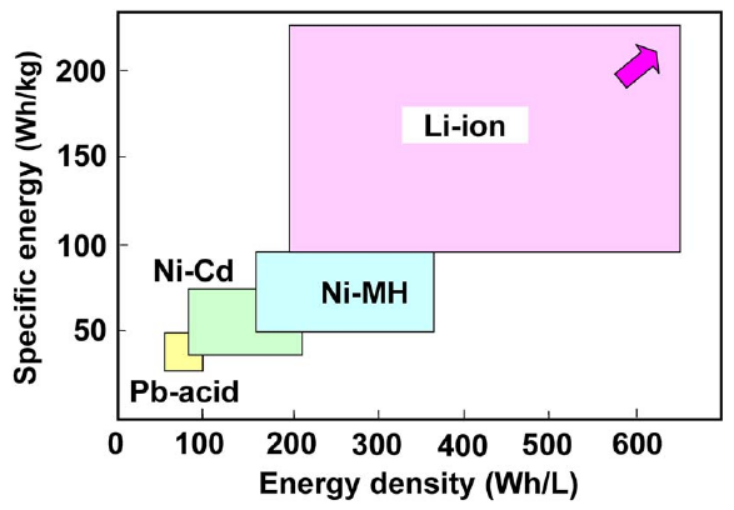
\includegraphics[width=0.6\textwidth]{comparisson-liion.png}
	\caption{Gr\'afica comparativa entre distintas tecnologías de baterías.}
	\label{comparisson_batt}
    \end{center}
\end{figure}

\noindent La aplicación práctica de las baterías de Litio-ion involucra la
integración de las mismas dentro de un sistema, involucrando un controlador
central (\acrshort{BMS}), sistemas de refrigeración, sensores y conectores entre
las celdas. En tales sistemas las celdas pueden conectarse de distintas formas,
por ejemplo, pueden conectarse en paralelo, para incrementar la capacidad del
pack, en serie, para incrementar el voltaje, o combinadas para lograr ambos
cometidos al mismo tiempo. Por ejemplo, un auto eléctrico de la marca
\emph{Tesla}, posee un pack de baterías de 85KWh compuesto por 7104 celdas, con
una arquitectura de 16 módulos conectados en serie , donde cada uno posee 444
celdas conectadas en paralelo.

%\newpage

\subsection{Modelado de bater\'ias de litio-ion}\label{litioModel}

\noindent Como se menciona anteriormente, las celdas de litio-ion son utilizadas
ampliamente en el mercado de consumo electr\'onico para un gran espectro de 
aplicaciones. Sin embargo, su fiabilidad y tiempo de vida son limitados y 
depende considerablemente de condiciones ambientales como también de su uso 
hist\'orico. Por lo tanto, se necesitan modelos de bater\'ias exactos y eficaces 
para que sean correctamente monitoreados por un \acrshort{BMS}.

\noindent Una celda, como se describe en la Secci\'on \ref{battery_fun}, puede 
ser caracterizada como un sistema electrotermoqu\'imico y actualmente existen 
una cantidad numerosa de modelos que logran describir el funcionamiento tanto 
est\'atico como din\'amico de la misma. Un modelo exacto y eficiente permite 
optimizar al m\'aximo el ciclo de vida de una bater\'ia ya que permite 
obtener informaci\'on sobre el \acrshort{SOC} como tambi\'en conocer 
par\'ametros cr\'iticos de la bater\'ia como por ejemplo, el perfil de descarga 
de la misma permitiendo ajustar los distintos algoritmos de protecci\'on y/o 
ecualizaci\'on que se apliquen en el desarrollo del \acrshort{BMS}.

A continuaci\'on se definen y se comparan los distintos modelos disponibles 
en la literatura actual. Esta comparaci\'on es basada en tres criterios:

\begin{description}
    \item [\textbf{Precisi\'on}:] La precisi\'on define cu\'an cercano un modelo
        puede predecir los valores de las variables de inter\'es de una
        bater\'ia.
    \item [\textbf{Complejidad}:] Se refiere a la cantidad de par\'ametros que
        necesita el modelo. Dependiendo de la complejidad del modelo, el 
        c\'alculo del mismo tomar\'a mayor o menor tiempo, cuestionando su 
        utilidad para una aplicaci\'on en tiempo real.
    \item [\textbf{Interpretaci\'on f\'isica}:] Esto se define como el nivel de
        interpretaci\'on anal\'itico que el modelo puede dar con respecto al
        funcionamiento interno de una bater\'ia.
\end{description}

\subsubsection{Modelos F\'isicos}\label{phyModel}

\noindent Los modelos f\'isicos, o tambi\'en conocidos como cajas blancas, son 
modelos de bajo nivel con un grado de exactitud muy alto. Permiten describir la 
estructura de los materiales y logran describir los complejos fen\'omenos 
electroqu\'imicos que suceden dentro de celda, tambi\'en denominados fen\'omenos 
termodin\'amicos, kin\'eticos y de transporte.

\noindent La bibliograf\'ia \cite{Schmidt2013} presenta un resumen del 
fen\'omeno f\'isico como se muestra en la Figura \ref{schmidt_fen_fis}. En ella, 
se pueden observar cuatro procesos en tres regiones de operaci\'on: las dos 
fases s\'olidas del material de los electrodos, y la fase l\'iquida del 
electrolito.

\begin{figure}[h!]
    \begin{center}
        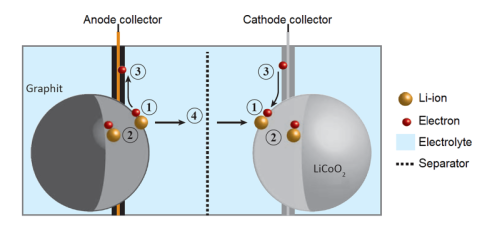
\includegraphics[width=0.7\textwidth]{schmidt_proceso_fisico.png}
        \caption{Descripci\'on gr\'afica del proceso interno de una celda de litio-ion.}
        \label{schmidt_fen_fis}
    \end{center}
\end{figure}

\noindent El primer proceso se denomina \emph{pasaje de cargas} y se da en 
la primer regi\'on de operaci\'on: la fase s\'olida del electrodo. 
Este proceso describe la intercalaci\'on como tambi\'en la desintercalaci\'on 
de los iones de litio dentro del material activo. El segundo proceso, ocurre 
en la misma regi\'on, y se la denomina la \emph{difusi\'on del estado s\'olido} 
de los iones de litio forzado por el gradiente de concentraci\'on de iones entre 
la superficie y el volumen del electrodo. El tercer proceso, se describe como 
la \emph{conducci\'on de electrones} entre un electrodo y otro a trav\'es de 
un circuito externo. Por \'ultimo, el cuarto proceso es la \emph{conducci\'on de 
iones} en el electrolito a trav\'es del separador, que tambi\'en es forzado for 
un gradiente de concentraci\'on y basado en la difusi\'on pero ocurre a mucha 
mayor velocidad que en los electrodos.

\noindent Estos tipos de modelos dependen de una gran cantidad de par\'ametros,
como tambi\'en de ecuaciones diferenciales interdependientes, para poder 
replicar el comportamiento de una celda se utilizan coeficientes de difusi\'on y 
propiedades de los materiales dentro de las ecuaciones dependientes del mismo. 
Los autores en \cite{Li2016} se basan en un modelo unidimensional a lo largo de 
la secci\'on de la celda, dividiéndolo en cinco secciones, aplicando las 
siguientes ecuaciones diferenciales: 

\begin{itemize}
    \item \textbf{Conservaci\'on de carga en un s\'olido homog\'eneo}
        \begin{equation}
            \nabla (-\sigma\nabla\upvarphi_s)=-j^{Li} 
            \label{Chrg_cons_hom_sol}
        \end{equation}	
    \item \textbf{Conservaci\'on de masa en un s\'olido homog\'eneo}
        \begin{equation}
            \frac{\partial c_s}{\partial t}=\nabla \cdot (D_s\nabla c_s) 
            \label{Mass_cons_hom_sol}
        \end{equation}	
    \item \textbf{Conservaci\'on de masa en un electrolito homog\'eneo}
        \begin{equation}
            \varepsilon_e\frac{\partial c_e}{\partial t} + \nabla \cdot
            (-D_e\nabla c_e) = \left(\frac{1-t_+^0}{F}\right)j^{Li}
            \label{Mass_cons_hom_electrolyte}
        \end{equation}	
    \item \textbf{Conservaci\'on de carga en un electrolito homog\'eneo}
        \begin{equation}
            \nabla \cdot (\upkappa \nabla \upvarphi_e + \upkappa_D \nabla \ln 
            c_e) = -j^{Li}
            \label{Chrg_cons_hom_electrolyte}
        \end{equation}	
    \item \textbf{Ecuaci\'on de Butler-Volmer:} Esta ecuaci\'on representa el
        movimiento de cargas en una uni\'on entre un s\'olido conductor y una
        soluci\'on de iones de litio con el efecto de doble capa
        \begin{equation}
            j^{Li} =
            a_si_0\left[{e^\frac{F\eta}{2RT}-e^{-\frac{F\eta}{2RT}}}\right] + 
            a_sC_{dl}\frac{\partial{(\upvarphi_s - \upvarphi_e)}}{\partial t}
            \label{Butler_Volmer_kinetics}
        \end{equation}	
\end{itemize}

En las ecuaciones \ref{Chrg_cons_hom_sol} - \ref{Butler_Volmer_kinetics}, se 
utilizan las siguientes variables:

\begin{description}
    \item [$\mathrm{\sigma}$]: Conductividad de la fase s\'olida del
        electrodo.
    \item [$\mathrm{\upvarphi_s}$]: Potencial el\'ectrico de la fase
        s\'olida.
    \item [$\mathrm{\upvarphi_e}$]: Potencial el\'ectrico del
        electrolito.
    \item [$\mathrm{j^{Li}}$]: Densidad de corriente producida por el
        consumo de iones de litio.
    \item [t]: Tiempo transcurrido.
    \item [c]: Concentraci\'on de iones de litio.
    \item [D]: Coeficiente de difusi\'on del material.
    \item [F]: Constante de Faraday.
    \item [$\mathrm{\varepsilon}$]: Fracci\'on por volumen.
    \item [$\mathrm{t_+^0}$]: N\'umero de transferencia.
    \item [$\mathrm{\upkappa}$]: Conductividad del electrolito.
    \item [$\mathrm{\upkappa_D}$]: Conductividad de la difusi\'on.
    \item [$\mathrm{i_0}$]: Corriente de intercambio.
    \item [$\mathrm{\eta}$]: Sobretensi\'on.
    \item [a]: \'Area espec\'ifica de la secci\'on.
    \item [$\mathrm{C_{dl}}$]: C\'apacidad de la doble capa.
\end{description}

A pesar de su alta exactitud, este tipo de modelo resulta complejo de
implementar en sistemas de tiempo real debido a la gran cantidad de ecuaciones
diferenciales a implementar con su extensa cantidad de par\'ametros a ajustar en
el mismo, imposibilitando su uso en veh\'iculos el\'ectricos.

\subsubsection{Modelos emp\'iricos}\label{empModels}

\noindent Los modelos emp\'iricos, tambi\'en conocidos como \emph{cajas negras},
son aquellos que describen a la batería en puntos de trabajo definidos y que
proveen pobres o incluso nulos conocimientos sobre el funcionamiento interno del
sistema, desconociéndose incluso el significado f\'isico de mucho de sus
par\'ametros internos del modelo. Las aproximaciones matem\'aticas que se
utilizan para definir la funci\'on transferencia entre las entradas y las
salidas de estos modelos permiten que los mismos sean f\'aciles de configurar
como tambi\'en generar predicciones y respuestas r\'apidas. Sin embargo, la
exactitud es limitada, especialmente si el modelo es muy simple, aunque puede
ser mejorado si se combina con un modelo de bajo nivel.

\subsubsection{Modelos abstractos}\label{absModels}

\noindent Tambi\'en conocidos como \emph{cajas grises}, los modelos abstractos 
proveen una representaci\'on alternativa de la entidad f\'isica a modelar. 
A pesar de que hay varias formas posibles de realizarlo, la m\'as utilizada 
dentro de la bibliograf\'ia es su representaci\'on en un circuito el\'ectrico 
equivalente. Los modelos basados en circuitos son simples y pr\'acticos porque 
permiten que el proceso electroqu\'imico que ocurre dentro de la celda sea 
reemplazado por un simple circuito. La correlaci\'on con las din\'amicas de la 
bater\'ia son preservados sin comprometer demasiada exactitud en su 
predicci\'on.

\noindent El costo de configuraci\'on para tales modelos es reducido en 
comparaci\'on a modelos de bajo nivel, sin embargo \'estos requiren de 
\emph{Look-up Tables} para coincidir con los datos experimentales. 
La complejidad de los mismos es m\'as flexible dependiendo de la unidad de 
c\'omputo como tambi\'en de la memoria disponible. Los mismo se pueden 
complejizar utilizando efectos de segundo \'orden, tales como la temperatura, 
degradaci\'on de la capacidad como tambi\'en el envejecimiento de las celdas.

\noindent A continuaci\'on se describen los modelos m\'as utilizados dentro de 
la literatura actual.

\subsubsubsection{Circuito simple}

\noindent El circuito el\'ectrico más simple que representa una bater\'ia de 
litio-ion es un circuito con constante de tiempo cero que se puede observar en 
la Figura \ref{zero_time_constant_sch}. Si el usuario no necesita representar la 
din\'amica de la bater\'ia, este modelo es capaz de representar el 
comportamiento est\'atico del sistema. 

\begin{figure}[h!]
    \begin{center}
        \begin{circuitikz}[american voltages]
            \draw 
                (0, 0) -- (3.5, 0)
                (0, 0) -- (0, .5)
                (0, 1.5) to[american voltage source, v_=$V_{OCV}$] (0, 0.5)
                (0, 1.5) -- (0, 2) to[R, l_=$R_S$] (3, 2) 
                to [short, i_=$I_{batt}$] (3.5, 2)
                (4, 2) to [open, v=$V_{batt}$] (4, 0);
        \end{circuitikz}
        \caption{Modelo de constante de tiempo cero para una celda de litio 
                 ion.}
        \label{zero_time_constant_sch}
    \end{center}
\end{figure}


\noindent El \acrshort{OCV} se relaciona directamente con el \acrshort{SOC},
definido en la Ecuación \ref{ocv_soc_ztc}

\begin{equation}
    SoC = \frac{C_{current}}{C_{full}}\dot 100\% \label{ocv_soc_ztc}
\end{equation}

\noindent Donde $\mathrm{C_{current}}$ es la cantidad de carga disponible en la 
celda y $\mathrm{C_{full}}$ es la capacidad de la celda cuando est\'a 
completamente cargada. La ecuaci\'on del modelo es expresada en la Ecuaci\'on 
\ref{vbatt_ocv_soc_ztc}.

\begin{equation}
    V_{batt} = V_{OC} - R_S \times I_{batt} \label{vbatt_ocv_soc_ztc}
\end{equation}

\noindent La curva del \acrshort{OCV} como funci\'on del tiempo muestra una 
caida del voltaje para ciertas condiciones de descarga. Los importantes 
par\'ametros que afectan el proceso de descarga son la corriente de descarga, 
la temperatura y la historia de carga/descarga.

\noindent El efecto de la temperatura en el proceso de descarga es visto a
temperaturas mucho más bajas que a temperatura ambiente, donde la actividad
qu\'imica disminuye y la resitencia de la bater\'ia aumenta. A temperaturas
m\'as altas que la ambiente, la resistencia interna disminuye, mejorando la
velocidad de la actividad qu\'imica, por lo tanto, y desafortunadamente,
induciendo un efecto de auto descarga.

\noindent La desventaja principal del modelo de constante de tiempo cero es que 
no contempla la din\'amica de las celdas. Sin embargo, esto puede ser mitigado 
de forma f\'acil agregando un tanque RC en serie a la resistencia (\emph{Fig.
\ref{one_time_constant_sch}}), que describe la respuesta din\'amica de la 
bater\'ia durante el proceso de carga/descarga.

\begin{figure}[h!]
    \begin{center}
        \begin{circuitikz}[american voltages]
            \draw 
                (0, 0) -- (7, 0)
                (0, 0) -- (0, 1)
                (0, 2) to[american voltage source, v_=$V_{OCV}$] (0, 1)
                (0, 2) -- (0, 3) to[R, l_=$R_s$] (3, 3) to[R, l_=$R_p$] (6, 3)
                (3, 3) to[short, *-] (3, 1.5) to [C, l_=$C_p$] 
                (6, 1.5) -- (6, 3) to [short, i_=$I_{batt}$] (7, 3)
                (7.5, 3) to [open, v=$V_{batt}$] (7.5, 0);
        \end{circuitikz}
        \caption{Modelo de primer \'orden para una celda de litio-ion.}
        \label{one_time_constant_sch}
    \end{center}
\end{figure}

\noindent La exactitud del modelo y su comportamiento din\'amico, pueden ser 
mejorados agregando m\'as tanques RC al circuito, esto a su vez incrementa la
complejidad del mismo. 

\subsubsubsection{Modelos basados en el espectro de impedancia}

La espectroscopía de impedancia electroquímica (\acrshort{EIS}, del ingl\'es
\acrlong{EIS}), es una técnica utilizada para describir las propiedades
eléctricas y dieléctricas de las celdas de ion-litio. También se la conoce como
Espectroscopía de Impedancia AC, debido a la que su implementación está
fundamentalmente basada en excitaciones de señales alternas.

La implementación de la EIS puede realizarse en modos distintos, excitando la
celda tanto con una señal de voltaje como con una señal de corriente.
Generalmente las señales de excitación son pequeñas señales sinusoidales, con lo
cual al excitar la celda por corriente podemos asegura la conservación del
estado de carga, ya que la integración en el largo plazo de la pequeña señal de
corriente es cero. Cuestion que no puede ser asegurada al ensayar la celda
exitada por tensión. La impedancia es calculada para señales de excitación con
diferentes frecuencias, que sean de interés en el espectro de análisis.

Para aplicar este m\'etodo, es necesario un sistema lineal invariante en el
tiempo. Por lo tanto, dado que las bater\'ias son sistemas altamente no lineales
durante el proceso de carga y descarga, el \acrshort{EIS} es aplicado a niveles
de \acrshort{SOC} donde la bater\'ia haya alcanzado un determinado estado de
relajación y reposo, para garantizar determinada linealidad necesaria.

\noindent La impedancia (Z) es una variable compleja representada en en el 
diagrama de Nyquist por una componente real y otra imaginaria. 
La Figura \ref{EIS_Nyquist} muestra un t\'ipico diagrama de Nyquist, 
como resultado de varias mediciones \acrshort{EIS} de una celda de litio-ion a
distintos niveles de \acrshort{SOC}. Cuantitativamente, los valores dependen de 
varios factores, como mencionamos anteriormente, la temperatura, 
el \acrshort{SOC} y la corriente de carga/descarga.

\begin{figure}[h!]
    \begin{center}
	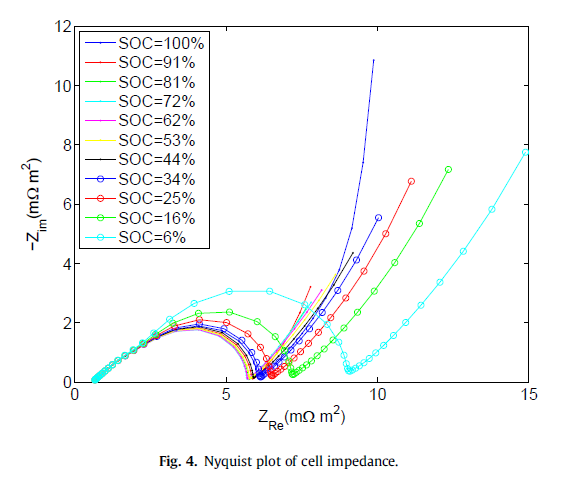
\includegraphics[width=0.4\textwidth]{EIS_Nyquist.png}
	\caption{Diagrama de Nyquist - Espectroscopía Dieléctrica (EIS) de 
	una batería de Li-Ion obtenida por barrido frecuencial.}
	\label{EIS_Nyquist}
    \end{center}
\end{figure}
\FloatBarrier

\noindent La curva puede ser subdividida seg\'un los rangos de frecuencia en
distintas secciones, como se puede observar en la Figura
\ref{EIS_nyquist_sections}. Estas secciones est\'an asociadas con fen\'omenos
f\'isicos y electroqu\'imicos bien definidos que ocurren dentro de la celda.

\noindent La secci\'on con $\mathrm{Z" < 0}$ consiste de tres \'areas bien
reconocibles. El arco a frecuencias muy bajas (cercanas a la corriente continua)
se asocia con el comportamiento de difusi\'on introducido en la Seccion
\ref{battery_fun} y es representado por la impedancia de \emph{estado s\'olido
de Warburg}. El segundo arco a frecuencias un poco m\'as altas (arco [ii] en
Fig.  \ref{EIS_nyquist_sections}) corresponde a la kin\'etica de la
transferencia de carga. El tercer y arco m\'as pequeño cerca del eje real (arco
[iii] en Fig.  \ref{EIS_nyquist_sections}) representa los efectos entre capas de
la interfaz s\'olida del electrolito.

\begin{figure}[h!]
    \begin{center}
	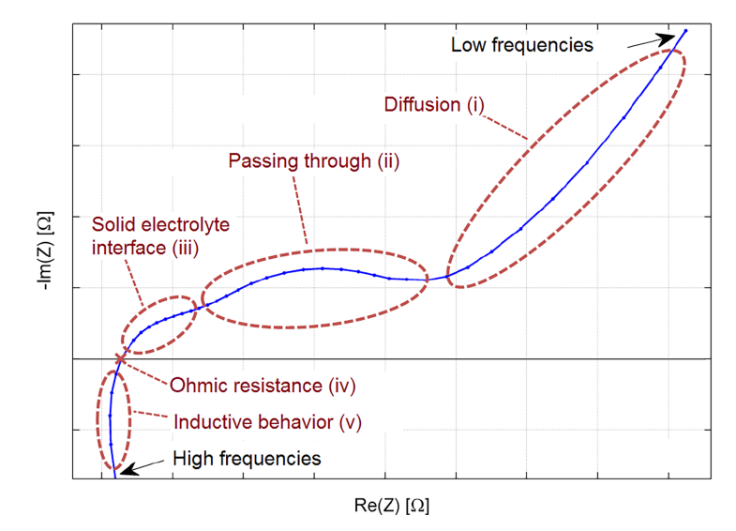
\includegraphics[width=0.7\textwidth]{EIS_nyquist_section.png}
	\caption{Secciones identificables dentro del diagrama de Nyquist.}
	\label{EIS_nyquist_sections}
    \end{center}
\end{figure}
\FloatBarrier

\noindent El punto (iv) de la Figura \ref{EIS_nyquist_sections} representa la 
resistencia \'ohmica total del sistema, incluyendo la resistencia del 
electrolito como tambi\'en la de los electrodos. Este punto generalmente occurre 
a una frecuencia dentro del rango de los KHz pero puede variar considerablemente 
con el diseño de la celda y los materiales utilizados.

\noindent Las altas frecuencias muestran un comportamiento inductivo con 
$\mathrm{Z" > 0}$ (secci\'on (v) de la Figura \ref{EIS_nyquist_sections}) 
correspondiente a la estructura porosa de los electrodos y los conectores de la 
bater\'ia.

\noindent El circuito equivalente de la respuesta de la impedancia es
introducido en \cite{Moss} y se puede observar en la Figura
\ref{sch_modelo_EIS}

\begin{figure}[h!]
    \begin{center}
        \begin{circuitikz}
            \draw
            (0, 0) to[L, o-, l=$L_s$] (2, 0) to [R, l=$R_s$] (4, 0) to[R,
            l=$R_{p1}$] (6, 0)
            (4, 0) to [short, *-] (4, -2) to [C, l=$C_{p1}$] (6, -2) to [short, -*]
            (6, 0) to[short, -*] (7, 0) to [C, l=$C_{dl}$] (11, 0)
            (7, 0) to[short] (7, -2) to[R, l=$R_{CT}$] 
            (9, -2) to[R, l=$Z(\omega)$] (11, -2) to[short, -*] (11, 0)
            to[C, -o, l=$C_{int}$] (12, 0);
        \end{circuitikz}
        \caption{Modelo equivalente a la respuesta del \acrshort{EIS}}
        \label{sch_modelo_EIS}
    \end{center}
\end{figure}
\FloatBarrier

\noindent Donde los componentes representan las siguientes partes f\'isica de 
la celda:

\begin{itemize}
    \item $\mathrm{C_{dl}}$: Capacitancia electroqu\'imica de doble capa
        de la celda.
    \item $\mathrm{R_{CT}}$: Resistencia a la corriente
        far\'adica
    \item $\mathrm{C_{int}}$: Capacitancia de intercalaci\'on
        correspondiente a la acumuluaci\'on de iones de litio dentro de la
        matriz del electrodo.
    \item $\mathrm{Z(\omega)}$: Impedancia de estado s\'olido de Warburg
        que depende de la frecuencia del ensayo.
\end{itemize}

\noindent En \cite{Moss} se sugiere la substituci\'on de la impedancia de 
difusi\'on de Warburg con una cadena de tanques RC. La nueva cadena no refleja 
la impedancia del elemento de Warburg pero representa una aproximaci\'on 
con una exactitud aceptable. Tomando esta aproximaci\'on en consideraci\'on, se 
valida el uso de modelos el\'ectricos para modelar celdas en un circuito 
compuesto por una fuente de tensi\'on con una resistencia $\mathrm{R_s}$ y una 
cadena de tanques RC conectadas en serie. Esto es solo posible gracias a las 
relaciones de Kramers-Kronig \cite{Schmidt2013}, que pueden ser aplicadas en 
redes equivalentes, y sugiere que distintos circuitos pueden tener una respuesta 
equivalente o similar sin tener la misma topolog\'ia. En otras palabras, la 
bater\'ia puede ser modelada con una topolog\'ia m\'as simple usando elementos 
que no tienen una directa interpretaci\'on f\'isica. Este modelo es v\'alido, 
porque tiene la misma respuesta en frecuencia, y es m\'as f\'acil de 
parametrizar.

\subsubsection{Comparaci\'on de modelos y su evaluaci\'on para aplicaciones
en veh\'iculos el\'ectricos}\label{compModels}

\noindent La Tabla \ref{table_comp_models} presenta una comparaci\'on de los
modelos seg\'un el criterio previamente explicado. Los modelos simples pueden
ser menos costosos desde un punto de vista computacional como tambi\'en en
desarrollo, a su vez, \'estos son más susceptibles a incertezas en los
par\'ametros del mismo. Por el otro lado, modelos complejos necesitan mayor
tiempo para resolver los algoritmos inherentes a ellos.  Dependiendo de la
aplicaci\'on, la extracci\'on del m\'etodo del modelo y usabilidad deben ser
evaluados antes de comenzar su desarrollo.  Dentro de un ambiente de
laboratorio, se puede invertir m\'as tiempo para extraer un modelo m\'as
preciso. Sin embargo, en el campo se necesitan resultados de forma r\'apida para
evaluar si las celdas son aptas para ser aplicadas en un veh\'iculo, por
ejemplo, en estos casos los modelos son utilizados para el desarrollo de un
\acrshort{BMS} como es lo que se busca en el presente trabajo. 

\noindent Tener una extensa comprensi\'on de la bater\'ia en estos casos no es
necesario, aunque puede resultar beneficioso. Dado que el mismo es embebido
dentro de una unidad de monitoreo en tiempo real, como puede ser un 
\acrshort{MCU} y/o \acrshort{FPGA}. Es m\'as conveniente que el modelo sea 
simple, para que los tiempos de c\'omputo no sean muy altos comprometiendo 
niveles aceptables de exactitud en los mismos. 

\begin{table}[h!]
\begin{center}
\begin{tabular}{@{}ccccc@{}}
\textbf{Modelos} & \textbf{Exactitud} & \textbf{Complejidad} &
\textbf{Interpretaci\'on f\'isica} & \textbf{Aplicaci\'on apropiada}\\
\hline
F\'isicos   & Muy alta  & \textgreater{}50 par\'ametros         & Alta
& diseño de de bater\'ias \\\hline Emp\'iricos & Media 
& 2 a 3 par\'ametros & Baja & Predicciones\\ 
\hline Abstractos & Media & 2 a 30 par\'ametros & Limitada & 
Monitoreo y diagn\'ostico
\end{tabular}
\caption{Resumen de la comparaci\'on entre modelos de celdas de litio-ion.}
\label{table_comp_models}
\end{center}
\end{table}

\subsection{Algoritmos de Estimaci\'on del Estado de Carga}\label{algSoc}

\noindent El \acrshort{SOC} es el equivalente a medir la cantidad de combustible
restante en un veh\'iculo convencional basado en combustibles f\'osiles. La
funci\'on principal de esta variable es comunicar de forma instintiva el estado
de la bater\'ia al conductor y, al mismo tiempo, evitar problemas tales como la
sobrecarga y sobredescarga del pack de bater\'ias, en otras palabras, mantener
el pack de bater\'ia dentro de la zona de operaci\'on segura como tambi\'en 
lograr mantener las celdas ecualizadas entre sí.

\noindent Esta tarea involucra el uso de sensores que permitan obtener las
señales de tensi\'on, corriente y temperatura de la bater\'ia para que el
circuito de control pueda procesarlos y computar el \acrshort{SOC},
usando uno de los algoritmos disponibles en la literatura actual que es
un tema en constante investigaci\'on debido al comportamiento no-lineal de las 
celdas de litio-ion inherentes a sus elementos electroqu\'imicos, que se ven 
afectados por condiciones internas y externas.

\noindent Cuando se menciona el \acrshort{SOC}, se refiere a la relaci\'on entre
la capacidad de corriente que queda en la bater\'ia con respecto a la capacidad
total bajo determinadas condiciones (temperatura, corriente de carga/descarga,
envejecimiento, entre otras), y su expresi\'on matem\'atica se puede observar en
la Ecuaci\'on \ref{eq_soc_int}

\begin{equation}
    SOC = \frac{Q_c}{Q}\times100\% 
    \label{eq_soc_int}
\end{equation}

\noindent Donde, desde el punto de vista de los veh\'iculos el\'ectricos,
$\mathrm{Q_c}$ es la energía residual de la bater\'ia en el momento que se
calcula, y su unidad es Ah (Ampere-hora); Q es la capacidad total de la
bater\'ia teniendo la misma unidad que $\mathrm{Q_c}$.

\noindent El hecho de que la bater\'ia dependa de varios factores, obliga a que
la Ecuaci\'on \ref{eq_soc_int} sea modificada, obteniendo la siguiente 
expresi\'on (\emph{eq. \ref{eq_soc_extended}}).

\begin{equation}
    SOC(t) = SOC(t_0) - \int_{t_0}^t \frac{\eta I}{C_n }d\tau
    \label{eq_soc_extended}
\end{equation}

\noindent En la Ecuaci\'on \ref{eq_soc_extended}, $\mathrm{C_n}$ es la 
capacidad nominal de la bater\'ia (en Ah), $\mathrm{\eta}$ es la eficiencia 
cul\'ombica de la celda e I es la corriente que circula sobre la celda en el 
intervalo de tiempo $[t_{0}, t]$.

\noindent Adem\'as del comportamiento de la celda, tambi\'en se debe modelar el
efecto de envejecimiento de la celda sobre el estado de carga, que puede ser
afectado por el ensamblado de la bater\'ia, temperatura, condiciones de
ventilaci\'on, corriente de auto-descarga, concentraci\'on de electrolitos, por
el otro lado, tambi\'en se lo relaciona con inconsistencias entre las distintas
celdas que componen el pack de bater\'ias, como por ejemplo, voltaje,
resistencia interna, capacidad y otros parf'ametros que afectan el 
envejecimiento del pack. La relaci\'on del envejecimiento y el \acrshort{SOC} se
ve reflejado por el \acrshort{SOH}, que es una variable que permite cuantificar
la antigüedad de una bater\'ia. La influencia del envejecimiento de la celda
sobre el \acrshort{SOC} se puede expresar en la Ecuaci\'on \ref{soc_soh}.

\begin{equation}
    SOC(t) = SOH(t) - DOD(t) \label{soc_soh}
\end{equation}

\noindent En la Ecuaci\'on \ref{soc_soh}, SOH(t) es el estado de salud. 
Cuando la bater\'ia es nueva, se considera que el SOH est\'a a un 100\%. 
Por el otro lado, el \acrshort{DOD} (del ingl\'es, \acrlong{DOD}) indica cuanto 
de la capacidad total de la bater\'ia puede ser descargado realmente, este valor 
se toma en cuenta cuando solo se puede descargar el 80\% de la capacidad total 
de la celda.

\noindent Basado en caracter\'isticas experimentales y te\'oricas, existen 
varios m\'etodos para estimar el \acrshort{SOC} y pueden ser clasificados dentro 
de tres grupos: Los m\'etodos tradicionales de estimaci\'on que se basan 
meramente en datos experimentales, m\'etodos modernos basados en teor\'ias de 
control y, por \'ultimo, m\'etodos basados novedosos basados en algoritmos
pertenecientes a lo que hoy se denomina la \emph{ciencia de datos}.

\subsubsection{M\'etodos tradicionales basados en experimentos}
\label{tradSocMeth}

Estos m\'etodos dependen exclusivamente de una interpretaci\'on de mediciones
directas e indirectas de la bater\'ia, como por ejemplo, la corriente, 
la tensi\'on, la temperatura e, inclusive, el c\'alculo de otras variables en
base a estos valores con respecto al \acrshort{SOC}, por lo general se
caracterizan por ser simples de implementar mostrando un alto grado de error del
modelo. 

\subsubsubsection{M\'etodo en base al voltaje de circuito abierto}
\label{ocv_section}

\noindent La medici\'on del voltaje de circuito abierto, u \acrshort{OCV} (del
ingl\'es \acrlong{OCV}), se basa en la relaci\'on entre la medici\'on de este 
voltaje y el \acrshort{SOC} representado en la Ecuaci\'on \ref{ocv_soc_eq}.

\begin{equation}
    V_{OC} = f(SOC) \label{ocv_soc_eq}
\end{equation}

\noindent Esta relaci\'on se determina realizando el experimento \acrshort{HPPC} 
(del ingl\'es, \acrlong{HPPC}) que consiste en descargar la bater\'ia con pulsos 
de corrientes equivalentes a un tercio de su capacidad comenzando desde el 
100\% de la bater\'ia hasta un 10\% de su capacidad en donde, despu\'es de cada 
pulso, se deja descansar a la celda por un un intervalo de 2 horas, permitiendo 
que la misma se equilibre de forma t\'ermica y electroqu\'imica antes de aplicar 
el pr\'oximo pulso de corriente. Durante el proceso de este ensayo, se toman 
mediciones de corriente y tensi\'on en bornes de la bater\'ia, permiti\'endo 
obtener una curva de \acrshort{OCV} vs \acrshort{SOC} como se puede observar en 
la Figura \ref{soc_ocv_paper}.

\begin{figure}[h!]
    \begin{center}
        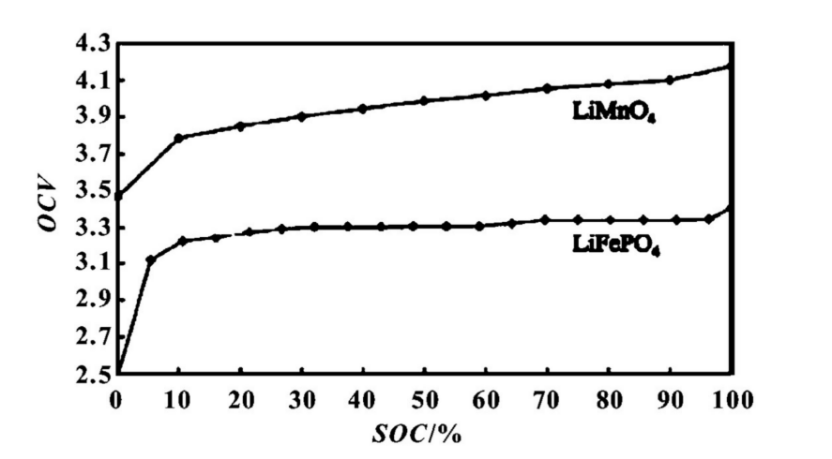
\includegraphics[width=0.6\textwidth]{soc_ocv_paper.png}
        \caption{Curva \acrshort{OCV} vs \acrshort{SOC} de una celda de hierro
        litio fosfato y otra de litio \'acido manganeso.}
        \label{soc_ocv_paper}
    \end{center}
\end{figure}

\noindent La ventaja del m\'etodo basado en la medici\'on del \acrshort{OCV} es
que es muy simple de implementar, solo hace falta tener una lectura de la
tensi\'on en bornes de la celda. Sin embargo, a pesar de su simpleza, el
m\'etodo no es apto para realizar una estimaci\'on en tiempo real debido a las
din\'amicas internas de la celda.

\noindent Por ejemplo, el voltaje de la celda tiene una respuesta muy din\'amica
ante fluctuaciones de corriente, como se puede observar en la Figura
\ref{relaxation_ocv}, lo que imposibilita utilizar este m\'etodo como estimador
del \acrshort{SOC} en tiempo real, ya que ante una pequeña circulaci\'on de
corriente la correlaci\'on entre el voltaje y el \acrshort{SOC} no es directa.

\begin{figure}[h!]
    \begin{center}
        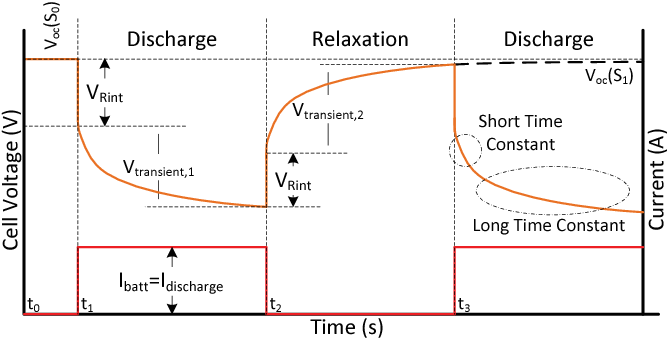
\includegraphics[width=0.7\textwidth]{ocv_relaxation.png}
        \caption{Repuesta de la tensi\'on de salida de una celda de Litio-ion
        ante un escal\'on de corriente}
        \label{relaxation_ocv}
    \end{center}
\end{figure}

\noindent Por el otro lado, las celdas de litio-ion poseen un voltaje de
hist\'eresis en el proceso de carga y descarga, como se puede observar en la
Figura \ref{histeresis_plot}, donde en la misma se muestrea el \acrshort{SOC}
para distintos per\'iodos de relajaci\'on, en ella se puede notar como
afecta el per\'iodo de relajaci\'on para realizar la estimaci\'on, donde a
mayor tiempo mejor es la estimaci\'on, esto se relaciona de forma directa con el
proceso de difusi\'on del litio dentro de la celda.

\begin{figure}[h!]
    \begin{center}
        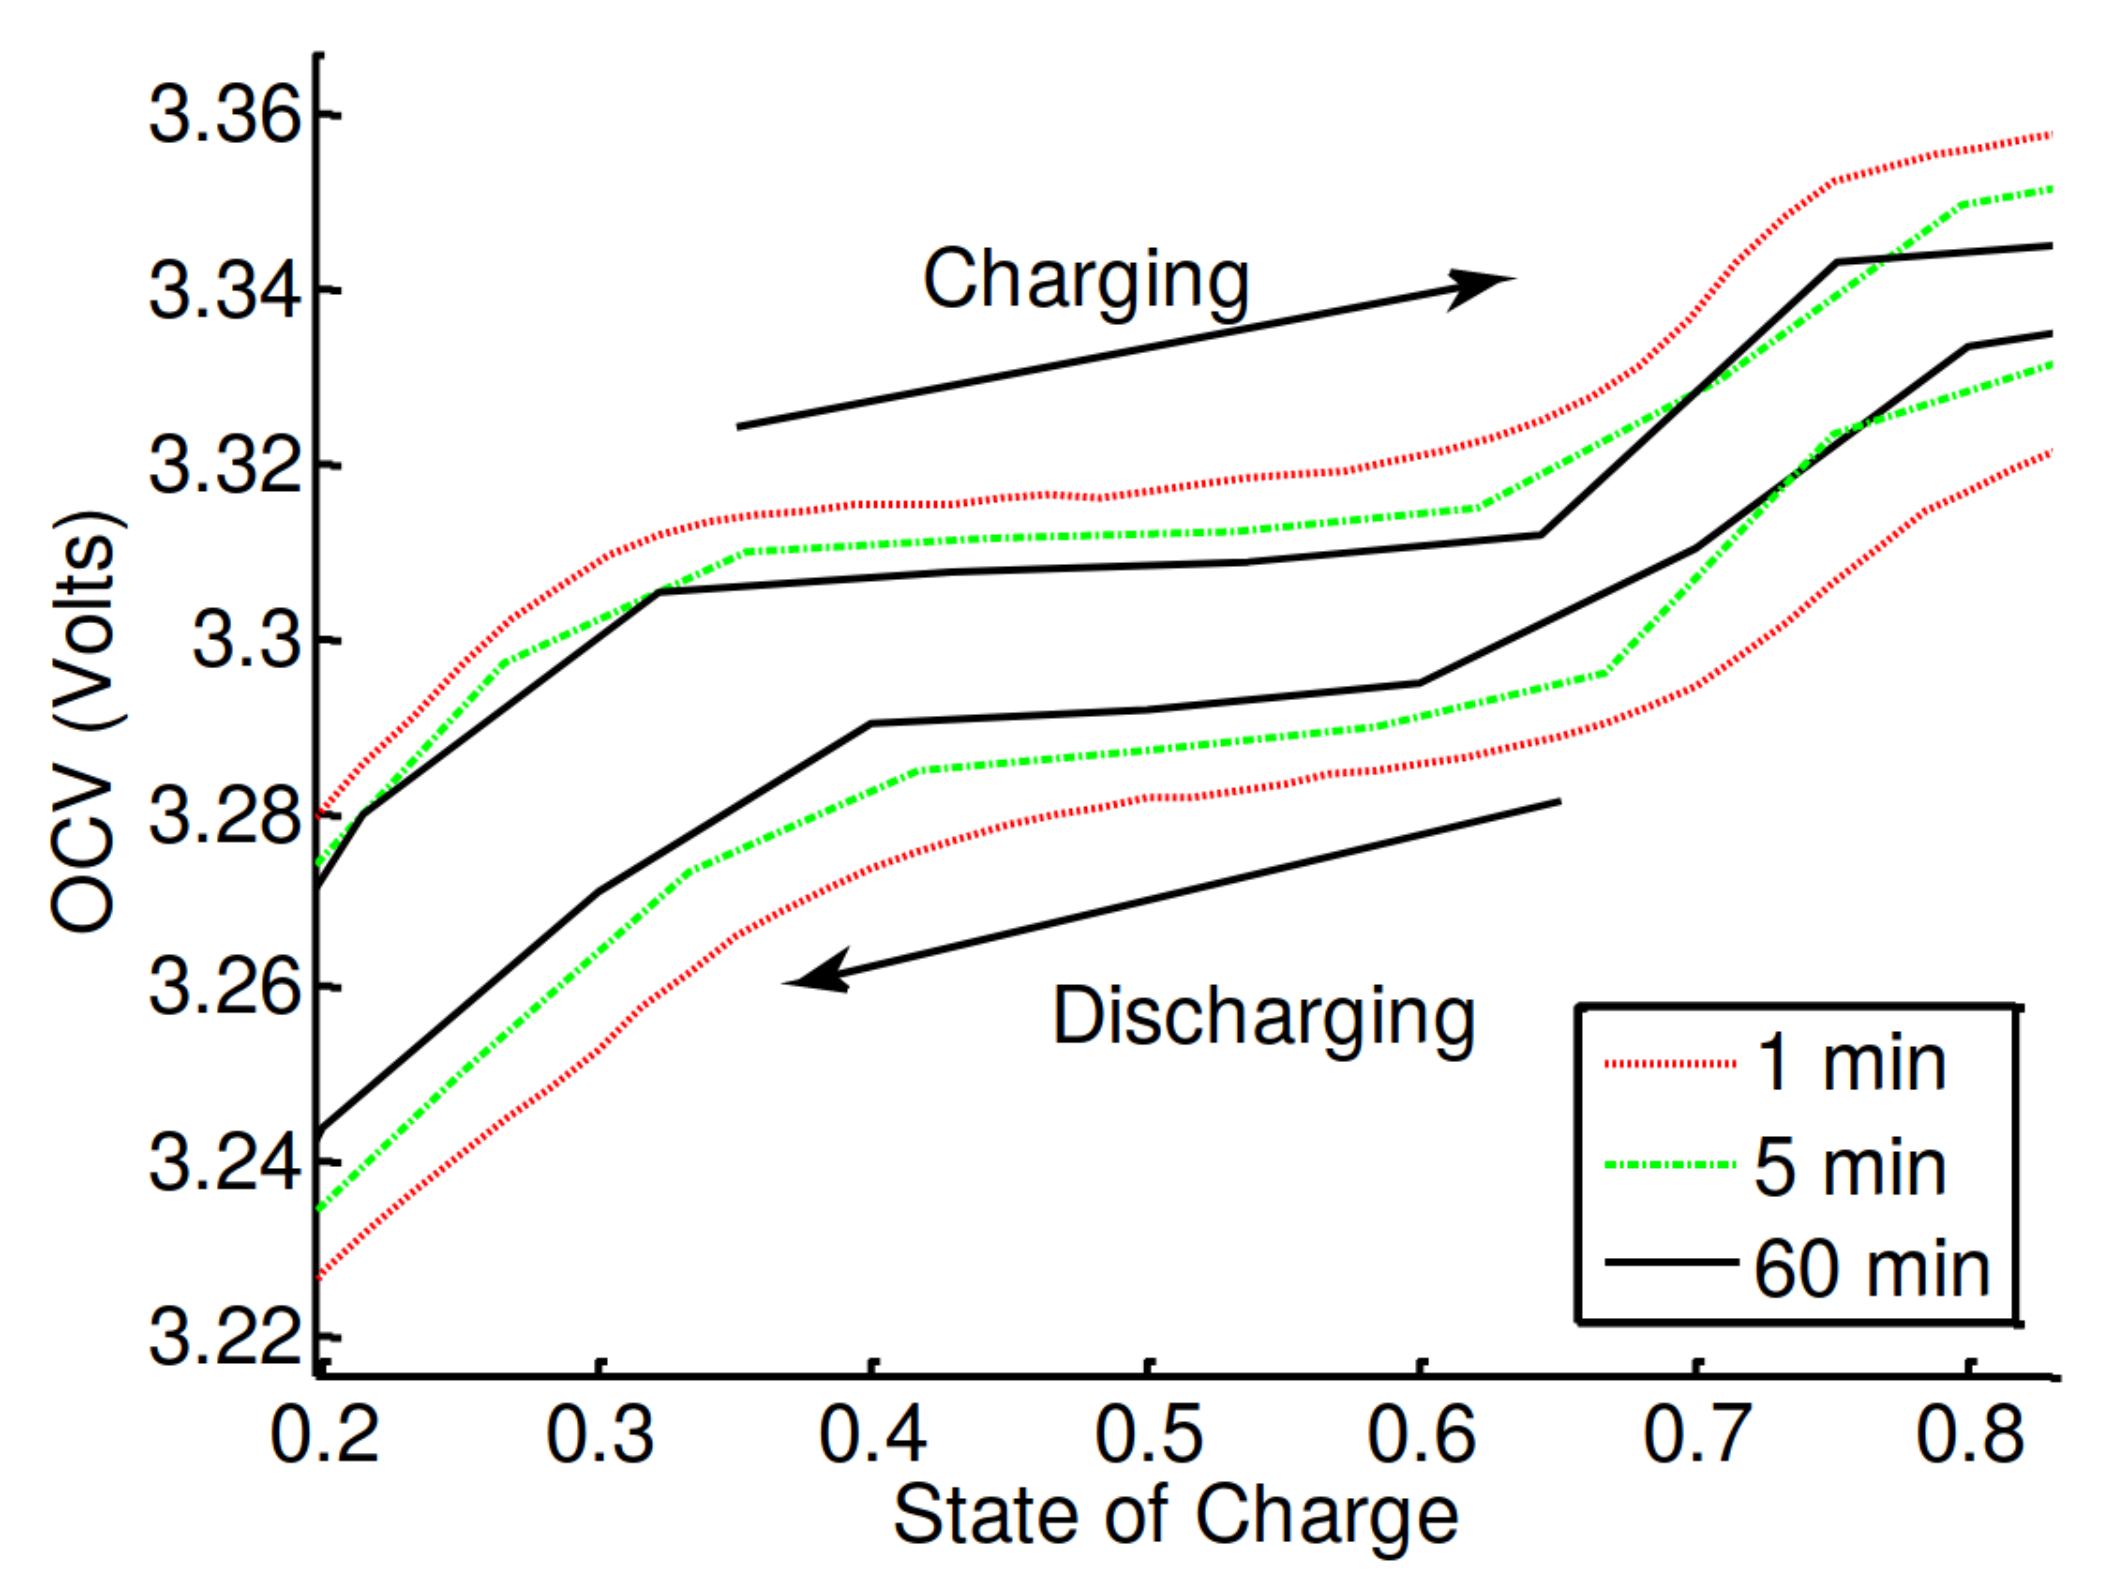
\includegraphics[width=0.5\textwidth]{soc_histeresis.png}
        \caption{curva \acrshort{OCV} vs \acrshort{SOC} durante el proceso de
            carga y descarga para distintos tiempos de relajaci\'on, denotando
            el fen\'omeno de hist\'eresis.} 
        \label{histeresis_plot}
    \end{center}
\end{figure}

\noindent Finalmente, la curva \acrshort{OCV} vs \acrshort{SOC} de la Figura
\ref{soc_ocv_paper} muestra secciones en la que la señal del \acrshort{OCV} es
plana ante una variaci\'on del \acrshort{SOC}, particularmente entre el 40\% y
el 60\%. Adem\'as, hay una variaci\'on muy pequeña en tensi\'on entre el 20\% y
80\%, lo cual, ante un m\'inimo error en la lectura de la tensi\'on de la celda
puede llevar a mediciones muy inexactas del \acrshort{SOC}. Estas observaciones
son los principales retos de estimar el \acrshort{SOC} utilizando solamente la
medici\'on del \acrshort{OCV}, lo cual llev\'o al desarrollo de nuevas
metodolog\'ias de estimaci\'on.

\newpage

\subsubsubsection{M\'etodo de integraci\'on de corriente}\label{ahMethod}

\noindent \'Este m\'etodo se basa en el c\'alculo de la circulaci\'on de 
corriente acumulada durante el proceso de carga y descarga de una bater\'ia. En 
la literatura se plantean varias versiones de la ecuaci\'on matem\'atica
utilizada por este m\'etodo, la m\'as utilizada se puede describir en la 
Ecuaci\'on \ref{ah_soc_general}.

\begin{equation}
    SOC = \frac{Q_0 + \int_{0}^t i_c\eta dt - \int_{0}^t i_d dt - S}{Q}
    \label{ah_soc_general}
\end{equation}

\noindent En la Ecuaci\'on \ref{ah_soc_general}, Q es la capacidad total de la 
bater\'ia, $\mathrm{Q_0}$ es la carga inicial de la celda, $\mathrm{\eta}$ es la 
eficiencia de carga, S es la cantidad estimada de auto-descarga de la celda, 
$\mathrm{i_c}$ es la corriente de carga e $\mathrm{i_d}$ es la corriente de 
descarga.

\noindent Por el otro lado, en \cite{ZHANG201524} tambi\'en se encuentran 
versiones mejoradas de \'este m\'etodo para corregir el error estimado. 
El principio de operaci\'on se puede observar en la Ecuaci\'on 
\ref{ah_soc_enhanced}.

\begin{equation}
    SOC = \alpha SOC_0 - \frac{1}{\delta c}\int \eta_\epsilon I dt
    \label{ah_soc_enhanced}
\end{equation}

En esta ecuaci\'on, $\mathrm{SOC_0}$ es obtenida por el m\'etodo de
\acrshort{OCV} descripto en la Secci\'on \ref{ocv_section}, $\mathrm{\alpha}$ es
el coeficiente que representa el factor de correcci\'on de auto-descarga y
envejecimiento de la celda, que se obtiene en base a varios experimentos en la
celda, $\mathrm{\delta}$ es el factor de correcci\'on por la capacidad de la
bater\'ia que se puede obtener a partir de la Ecuaci\'on
\ref{batt_cap_correction}. El par\'ametro $\mathrm{\eta_\epsilon}$ es la
eficiencia cul\'ombica equivalente de la celda, cuyo valor se obtiene unificando
la eficiencia cul\'ombica de distintas corrientes.

\begin{equation}
    \delta = 0.0010N^2 - 0.032N + 11.8819\label{batt_cap_correction}\;
    \text{donde N es el n\'umero de ciclos}
\end{equation}

\noindent El m\'etodo de integraci\'on de corriente tiene la ventaja de ser un
c\'alculo simple, estable y permite ser implementado en tiempo real.
Considerando la auto-descarga, temperatura, eficiencia de carga y descarga, el
m\'etodo puede alcanzar niveles de exactitud aceptables para una
implementaci\'on r\'apida en la estimaci\'on del \acrshort{SOC} en un BMS. Sin
embargo, este m\'etodo tiene dos principales desventajas:

\begin{enumerate}
    \item Dado que solo se integra corriente en un largo per\'iodo de tiempo, el
        m\'etodo es propenso a acumular considerable error en el tiempo.
    \item El mismo no logra eliminar la p\'erdida de la capacidad de carga como
        consecuencia del envejecimiento de la celda.
\end{enumerate}

\noindent Por esto mismo, varias bibliograf\'ias proponen fusionar el m\'etodo
por \acrshort{OCV} junto a \'este para compensar los errores inherentes, as\'i
obteniendo una metodolog\'ia simple y eficiente para estimar el \acrshort{SOC}
de una celda.

\subsubsubsection{Medici\'on de resistencia interna}\label{internalRMethod}

\noindent Este m\'etodo tiene el objetivo de relacionar la resistencia interna
de una celda con el \acrshort{SOC}, considerando la corriente de descarga y la
resistencia interna de la bater\'ia. Sin embargo, en la pr\'actica, la
relaci\'on entre los par\'ametros de una celda y el \acrshort{SOC} es bastante
compleja. En la etapa inicial y final de la descarga, la resistencia interna
aumenta considerablemente obteniendo como resultado grandes fluctuaciones,
mientras que durante el resto del proceso de descarga la resistencia interna se
caracteriza por una meseta, debido a ello, \'este m\'etodo es generalmente
implementado durante el principio y el final del proceso de descarga. Este 
comportamiento se puede observar en la Figura \ref{res_int_graph}.

\begin{figure}[h]
    \begin{center}
	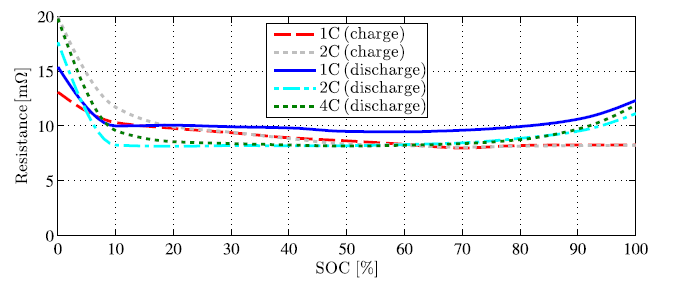
\includegraphics[width=0.7\textwidth]{Ro_vs_SOC.png}
	\caption{Resistencia en corriente continua de una batería de litio-ion vs. 
        SOC obtenida por HPPC}
	\label{res_int_graph}
    \end{center}
\end{figure}

\noindent La resistencia interna de una bater\'ia puede ser dividida en la
resistencia de corriente alterna y corriente continua. Por lo tanto,
\'este m\'etodo puede ser dividido en dos m\'etodos para cada una. 
La impendancia en alterna es la funci\'on transferencia entre el
voltaje y la corriente de la celda cuando se le aplica una corriente
alterna y ambos pueden ser medidos f\'acilmente con un medidor de impedancias. 
Sin embargo, a pesar de ser un m\'etodo muy simple de implementar, la relaci\'on 
de la resistencia interna con el SOC se acomplejiza dependiendo de la 
tecnolog\'ia de la bater\'ia, especialmente en las celdas de litio-ion.

\noindent El m\'etodo consiste en excitar la bater\'ia por breves instantes 
(menores a 10ms) con un pulso de corriente, asumiendo que este per\'iodo es lo 
suficientemente acotado para que la variaci\'on de tensi\'on sea atribuida a la 
resistencia interna y no a la carga/descarga de la bater\'ia, el c\'alculo de la 
resistencia se podr\'ia obtener seg\'un la Ecuaci\'on
\ref{rint_batt_eq}:

\begin{equation}
    \frac{\Delta V}{\Delta I} = R_{\ohm} \label{rint_batt_eq}
\end{equation}

Sin embargo, a pesar de su simpleza, este m\'etodo no resulta atractivo para
implementar en sistemas en tiempo real dado que, como se menciona anteriormente,
tiene una gran exactitud \'unicamente en bajos y altos valores de \acrshort{SOC},
adem\'as, tambi\'en debe inyectarse una corriente de valor conocido para poder
estimar su valor, resultando en mayor complejidad al circuito del
\acrshort{BMS}, dado que debe generar esta corriente constante de forma
peri\'odica y en tiempo real.

\noindent En resumen, los m\'etodos de estimaci\'on del \acrshort{SOC} basados
en experimentos, como se menciona anteriormente, tienen la ventaja de ser 
simples y f\'aciles de implementar, pero requieren de mucha inversi\'on 
experimental en las celdas en relaci\'on al bajo rendimiento que proveen en 
estimar de forma exacta el \acrshort{SOC}. Con respecto a la exactitud de 
estimaci\'on y caracter\'isticas de los ensayos de cada m\'etodo, se puede decir 
que:

\begin{itemize}
    \item \textbf{Estimaci\'on por OCV:} La exactitud de este m\'etodo depende
        exclusivamente del tiempo en el que la bater\'ia estuvo relajada,
        mientras mayor sea este tiempo m\'as exacto es la estimaci\'on.
    \item \textbf{Estimaci\'on por integraci\'on de corriente:} Es
        principalmente utilizado para determinar el \acrshort{SOC} inicial, pero
        su exactitud disminuye con el tiempo de medici\'on, debido a que la
        resistencia interna cambia constantemente y es propenso a acumular
        errores.
    \item \textbf{M\'etodo de resistencia interna:} \'Este m\'etodo es solo
        estable sobre la etapa final e inicial de descarga y tiene un alto grado 
        de precisi\'on, pero el tiempo de ensayo no se puede obtener de forma
        precisa por lo que genera un error en el mismo.
\end{itemize}


\subsubsection{M\'etodos modernos basados en la teor\'ia de control}
\label{controlTheoryMethod}

\noindent Dentro de la ingenier\'ia y las matem\'aticas, la teor\'ia de control
se encarga de modelar y controlar la din\'amica de un sistema,
independientemente de su naturaleza. Cuando una o m\'as variables de salida
necesitan seguir determinada referencia, un controlador manipula las entradas
del mismo para que el sistema pueda lograr el efecto deseado a su salida.

\noindent La mayor\'ia de los conceptos de la teoría de control modena
encuentran su fundamento en la posibilidad de medir las variables de interes del
sistema, de forma directa o indirecta, a partir de sensores y trasductores
eléctricos. Desafortunadamente, tal suposici\'on no siempre es v\'alida. Los
sensores f\'isicos siempre tienen limitaciones que afectan estos sistemas. Por
ejemplo, en algunos casos los sensores son componentes muy costosos tanto
econ\'omicamente como en su implementaci\'on, en otros casos la variable a medir
no puede ser accesible o f\'isicamente medible debido a ambientes hostiles.
Finalmente, los sensores inducen errores significativos, tales como el ruido,
retardo de fase, errores determin\'isticos y respuesta limitada en ancho de
banda.

\noindent Para mitigar este problema, se plantea el uso de \emph{observadores}. 
Los observadores son algoritmos que combinan señales que provienen de sensores 
con conocimientos del sistema para producir señales \emph{observadas}. 
\'Estas señales pueden ser igual de exactas que el sensado, menos costosas de 
producir, y de mayor confianza que las señales proveniente de sensores. 
Los observadores ofrecen al diseñador la alternativa de agregar nuevos 
sensores, o mejorar los existentes agregando solamente costo computacional, sin 
reimplementaciones de hardware ahorrando traer altos costos de diseño durante la
etapa de desarrollo de un producto.

\noindent El principio de operaci\'on de un observador se basa en combinar la
medici\'on de salida de la planta con conocimientos previos de los distintos 
componentes que modelan a la misma, obteniendo un mayor conocimiento sobre el 
comportamiento de la planta a comparaci\'on de utilizar solamente la señal de 
salida de la misma. Como se puede observar en la Figura \ref{role_observer}, el 
observador aumenta la capacidad del sensor de salida y provee una señal de 
realimentaci\'on a las leyes de control.

\begin{figure}[h!]
    \begin{center}
    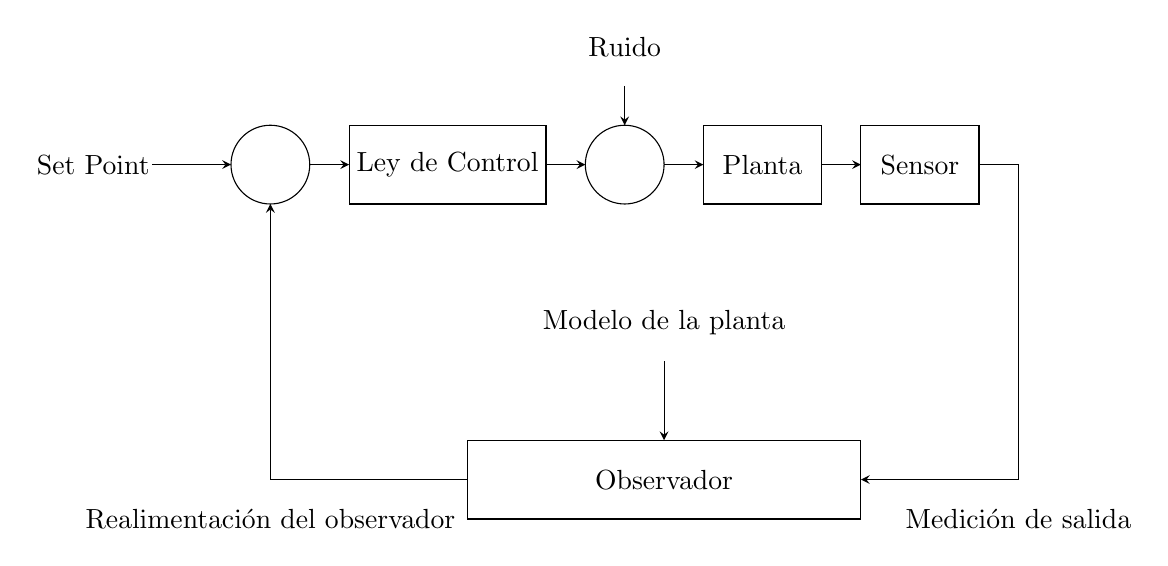
\begin{tikzpicture}
        \draw (-.75, 0) node {Set Point};
        \draw[-stealth] (0, 0) -> (1, 0);
        \draw (1.5, 0) circle (0.5);
        \draw[-stealth] (2, 0) -> (2.5, 0);
        \draw (2.5, .5) rectangle (5, -.5) node[pos=.5]{Ley de Control};
        \draw[-stealth] (5, 0) -> (5.5, 0);
        \draw (6, 0) circle (0.5);
        \draw[-stealth] (6, 1) -> (6, 0.5);
        \draw (6, 1.5) node {Ruido};
        \draw[-stealth] (6.5, 0) -> (7, 0); 
        \draw (7, .5) rectangle (8.5, -.5) node[pos=.5]{Planta};
        \draw[-stealth] (8.5, 0) -> (9, 0);
        \draw (9, .5) rectangle (10.5, -.5) node[pos=.5]{Sensor};
        \draw (10.5, 0) -> (11, 0) -> (11, -4);
        \draw[-stealth] (11, -4) -- (9, -4);
        \draw (11, -4.5) node {Medici\'on de salida};
        \draw (9, -3.5) rectangle (4, -4.5) node[pos=.5]{Observador};
        \draw[-stealth](6.5, -2.5) -- (6.5, -3.5);
        \draw (6.5, -2) node {Modelo de la planta};
        \draw (4, -4) -- (1.5, -4);
        \draw (1.5, -4.5) node {Realimentaci\'on del observador};
        \draw[-stealth] (1.5, -4) -- (1.5, -.5);
    \end{tikzpicture}
    \caption{Rol del observador en un sistema de control}
    \label{role_observer}
    \end{center}
\end{figure}
\FloatBarrier

\noindent Sin embargo, la tecnolog\'ia del observador no necesariamente es la
soluci\'on final a estos problemas. Como mencionamos anteriormente, los
observadores agregan trabajo computacional al producto final y, adem\'as, la
robustes de los mismos, en comparación con un sensor equivalente, depende pura y
exclusivamente de la complejidad matemática del observador, especialmente cuando
la planta sufre modificaciones substancialles al evolucionar alrededor del punto
de operaci\'on. 

\noindent Dentro de los observadores disponibles, la bibliograf\'ia relacionada
a la estimaci\'on del \acrshort{SOC} hace un gran \'enfasis en la utilizaci\'on
del \emph{filtro de Kalman} como un buen candidato (\cite{spagnol_kalman}, 
\cite{zhihao_kalman} y \cite{atsushi_kalman}) obteniendo resultados
prometedores. A continuaci\'on se desarrolla su principio de funcionamiento, 
beneficios y como se utiliza como observador del \acrshort{SOC}.

\subsubsubsection{M\'etodo del Filtro de Kalman}\label{KalmanFilterMethod}

\noindent Dentro de las herramientas matem\'aticas que pueden ser utilizadas 
para estimaci\'on de variables a partir de mediciones ruidosas, una de las m\'as
conocidas y usadas es el \emph{Filtro de Kalman} \cite{kalman_filter_paper}. 
Esencialmente, el filtro de Kalman es un conjunto de ecuaciones matem\'aticas 
que implementan un estimador de tipo \emph{predictor-corrector} que es \'optimo 
en el sentido de que minimiza la covarianza del error dadas determinadas 
condiciones y, a pesar de que estas condiciones son rara vez dadas, se obtienen 
buenos resultados para varias aplicaciones.

\noindent En principio, el filtro logra estimar la variable de inter\'es usando 
un control de retroalimentaci\'on: El filtro estima el estado del proceso en 
determinado instante de tiempo y despu\'es obtiene la realimentaci\'on en forma 
de mediciones ruidosas, en base a esta realimentaci\'on, calcula el error y
reacomoda su ganancia para disminuir el mismo. Las ecuaciones del filtro se
dividen en dos grupos: \emph{ecuaciones de actualizaci\'on en el tiempo} 
y \emph{ecuaciones de actualizaci\'on de medici\'on}. El primer conjunto de
ecuaciones es responsable de proyectar la estimaci\'on el estado actual y la
covarianza del error en el tiempo, para obtener estimaciones \emph{a priori}. 
El segundo conjunto de ecuaciones son responsables de la realimentaci\'on, por 
ejemplo, incorporando nuevas mediciones dentro del estado estimado de forma 
\emph{a priori} para obtener una estimaci\'on \emph{a posteriori} mejorada.

\noindent Las ecuaciones de actualizaci\'on del tiempo tambi\'en pueden ser 
interpretadas como ecuaciones de \emph{predicci\'on}, mientras que las 
ecuaciores de actualizaci\'on de medici\'on pueden ser interpretadas como 
ecuaciones de \emph{correcci\'on}. Obteniendo como resultado, un algoritmo 
recursivo de tipo \emph{predictor-corrector} para resolver problemas num\'ericos 
como se puede observar en la Figura \ref{kalman_filter_sch}.

\begin{figure}[h!]
    \begin{center}
    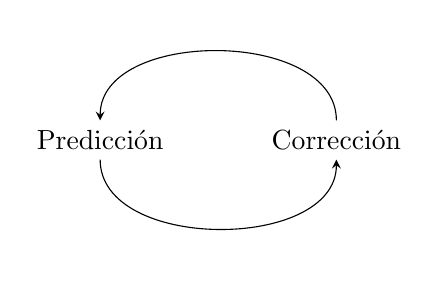
\begin{tikzpicture}
        \draw (0, 0) node {Predicci\'on};
        \draw[-stealth] (0, -.25) to[out=-90, in=-90] (3, -.25);
        \draw (3, 0) node {Correcci\'on};
        \draw[stealth-] (0, .25) to[out=90, in=90] (3, .25);
    \end{tikzpicture}
    \caption{El ciclo perpetuo del filtro de Kalman. }
    \label{kalman_filter_sch}
    \end{center}
\end{figure}
\FloatBarrier

La actualizaci\'on en el tiempo proyecta el estado actual. Mientras que la
actualizaci\'on de medici\'on ajusta la proyecci\'on estimada previamente a una
actual medici\'on a ese instante.

Las ecuaciones específicas para la estimaci\'on del estado (o actualizaci\'on en
el tiempo) se representan en las Ecuaciones \ref{est_state} y \ref{est_uncert}.

\begin{align}
    \hat{x}_{n+1, n} &= F\hat{x}_{n,n} + Gu_n & & \textrm{Estimaci\'on de estado}
    \label{est_state} \\
    P_{n+1,n} &= FP_{n,n}F^T + Q & & \textrm{Estimaci\'on de incerteza}
    \label{est_uncert}
\end{align}

\noindent Donde F es una matriz (n x n, donde n es la cantidad de estados del 
sistema) que relaciona la proyecci\'on del estado con el estado actual, G es una 
matriz (n x l, donde l es la cantidad de entradas del sistema) que relaciona las 
señales de entrada con la proyecci\'on del estado del sistema y, por \'ultimo, 
Q (n x n) es la covarianza del ruido relacionado al proceso interno del sistema.

\noindent En las ecuaciones anteriores se puede observar como se proyecta el 
estado y la covarianza desde el paso n al paso n+1, obteniendo una predicci\'on 
del estado del sistema.

\noindent Por el otro lado, las ecuaciones relacionadas a la actualizaci\'on de 
las mediciones se pueden observar en las Ecuaciones \ref{kalman_gain},
\ref{estimate_w_measurement} y \ref{estimate_uncertainty}.

\begin{align}
    K_n &= P_{n, n-1}H^T(HP_{n,n-1}H^T + R_n)^{-1} & & \textrm{Ganacia de Kalman}
    \label{kalman_gain}\\
    \hat{x}_{n, n} &= \hat{x}_{n,n-1} + K_n \left(z_n - H\hat{x}_{n, n-1}\right) & & \textrm{Actualizaci\'on del estado}
    \label{estimate_w_measurement}\\
    P_{n, n} &= \left(I - K_nH\right)P_{n,n-1}\left(I - K_nH\right)^T + K_n R_{n} K_n^T & & \textrm{Actualizaci\'on de la covarianza}
    \label{estimate_uncertainty}
\end{align}
\FloatBarrier

\noindent Donde H es una matriz (z x n, donde z es la cantidad de mediciones y n
es la cantidad de estados del sistema) que indica la relación entre las
mediciones y el vector de estado al momento n, en el supuesto ideal de que no
hubiera ruido en las mediciones. y R es una matriz (z x z, donde z es la
candidad de mediciones) de covarianza del ruido de las mediciones (depende de la
resolución de los sensores utilizados).

\noindent La primer tarea durante el proceso de \emph{correcci\'on} es calcular 
la ganancia de Kalman, $\mathrm{K_k}$, despu\'es el algoritmo procede a medir el
proceso obteniendo la variable $\mathrm{z_k}$, y con esta informaci\'on generar
el estado \emph{a posteriori} incorporando las mediciones como se puede observar
en la Ecuaci\'on \ref{estimate_w_measurement}, que es similar a la Ecuaci\'on
\ref{est_state} pero con mediciones actuales utilizando la ganancia de Kalman
como un corrector. Por \'ultimo se obtiene una estimaci\'on del error de
covarianza \emph{a posteriori} como se realiza en la Ecuaci\'on
\ref{estimate_uncertainty}. 

\noindent Para cada instante de tiempo y medici\'on, el proceso se repite con 
estimaciones previas usadas para proyectar o predicir nuevo estados. Esta 
naturaleza recursiva es una de las caracter\'isticas atractivas del filtro de 
Kalman, a comparaci\'on de, por ejemplo, un filtro de Wiener \cite{brown_hwang} 
que es diseñado para operar con toda la informaci\'on en cada estimaci\'on. 
En cambio, el filtro de Kalman, utiliza, de forma recursiva, las mediciones 
pasadas para estimar el estado actual. La Figura \ref{complete_kf} muestra la 
operaci\'on del fitro, combinando un diagrama de alto nivel combinando las 
ecuaciones \ref{est_state}-\ref{estimate_uncertainty}.

\begin{figure}[h!]
    \begin{center}
        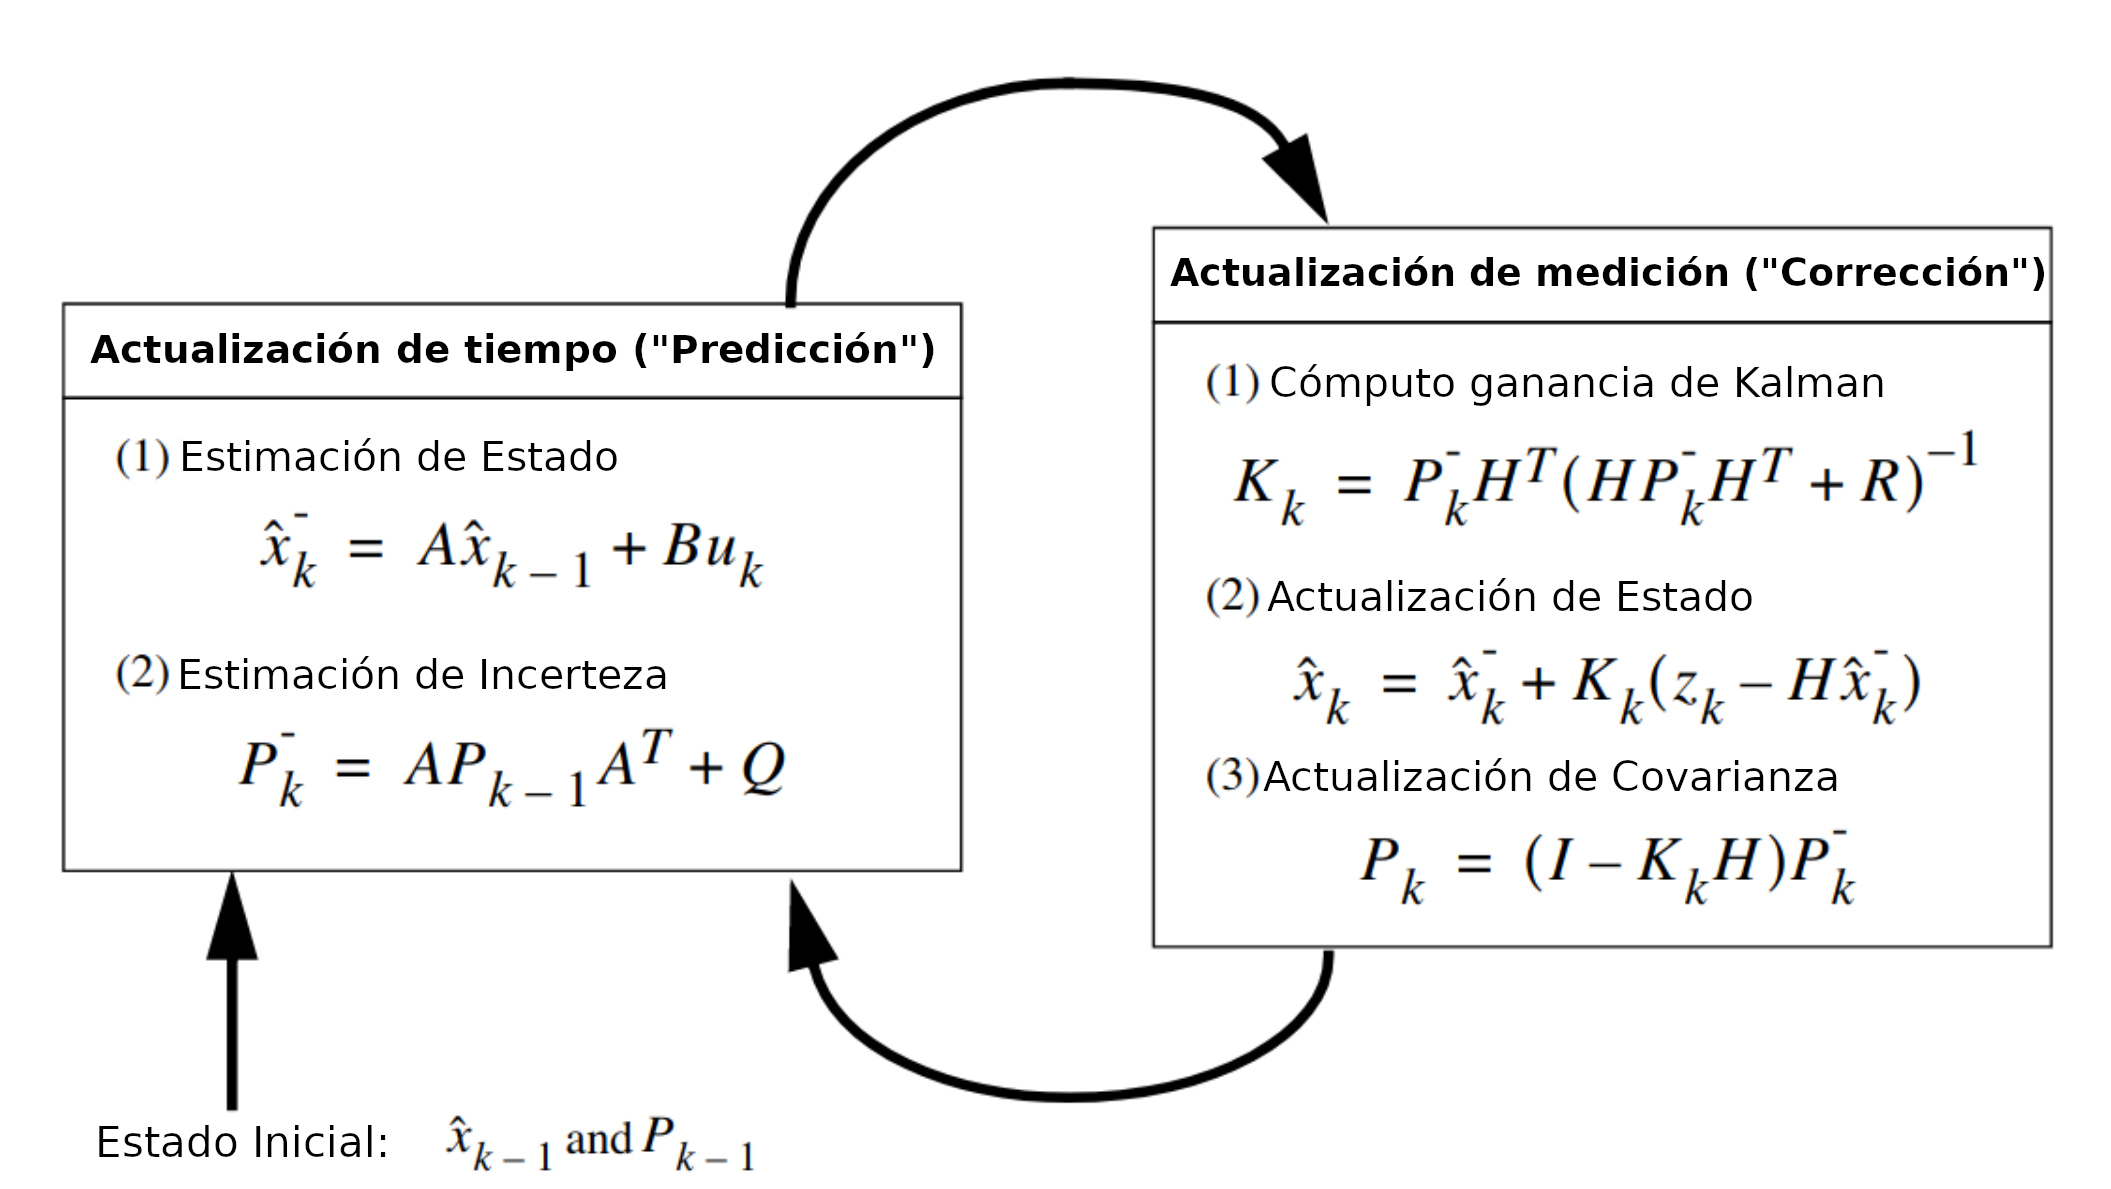
\includegraphics[width=0.7\textwidth]{kf_complete_esp.png}
        \caption{Diagrama detallado del funcionamieno del filtro de Kalman}
        \label{complete_kf}
    \end{center}
\end{figure}
\FloatBarrier

Resumiendo las matrices y vectores enunciadas en la Figura \ref{complete_kf}:

\begin{description}
    \item [$\mathbf{A_{k}}$]: Matriz de transición de estados. Es la matriz que
        relaciona $\mathbf{\hat{x}_{k}}$ con $\mathbf{\hat{x}_{k-1}}$.
    \item [$\mathbf{\hat{x}_{k}}$]: Estimado a priori del Vector de Estados.
    \item [$\mathbf{P_{k}}$]: Covarianza del error asociada a la estimación a priori.
    \item [$\mathbf{z_{k}}$]: Vector de mediciones al momento k.
    \item [$\mathbf{H_{k}}$]: Matriz de relación entre las mediciones z y el vector de
        estado al momento k.
    \item [$\mathbf{R_{k}}$]: Matriz de covarianza del ruido de las mediciones.
\end{description}

El desarrollo matemático completo del filtro de Kalman se incluye como apendice
en Anexo \ref{matKalman} para su consulta.

\noindent Este m\'etodo puede ser f\'acilmente utilizado para estimar el 
\acrshort{SOC} de una celda. En principio se necesita un modelo linealizado de la 
celda de litio-ion representado en un sistema de ecuaciones de estado e 
implementar el filtro para poder estimar el \acrshort{SOC} tomando una variable 
que se pueda utilizar y medir como salida para poder calcular un error de la 
estimaci\'on del estado, de forma tal que el algoritmo pueda iterar y calcular 
la ganancia de Kalman para \emph{corregir} su estimaci\'on.

\noindent Por ejemplo, en \cite{spagnol_kalman} se propone implementar un filtro 
de Kalman utilizando un modelo en ecuaciones de estado que permite fusionar la
representaci\'on de la celda en un modelo el\'ectrico (t\'ipico para
estimaci\'on del \acrshort{OCV}) con metodolog\'ias de conteo de Coulomb
(desarrollada en \ref{ahMethod}) obteniendo un m\'etodo que permite rechazar
tanto el ruido de las mediciones como tambi\'en errores param\'etricos del
modelo.

\noindent Los autores plantean el uso de un modelo el\'ectrico de la bater\'ia
basado en dos tanques RC conectados a una resistencia en serie y dos fuentes de
tensi\'on, controladas por el \acrshort{SOC}, que representa el \acrshort{OCV} 
de la celda durante el proceso de carga y descarga, como se puede observar en la 
Figura \ref{2rc_circuit}.

%\newpage

\begin{figure}[h!]
    \begin{center}    
        \begin{circuitikz}[american voltages]
            \draw (0, 0) to[D*] (0, -2);
            \draw (0, -2) to[cV, l=$OCV_{CC}(SoC)$] (0, -4);
            \draw (-1.5, -2) to[D*] (-1.5, 0);
            \draw (-1.5, -2) to[cV, l_=$OCV_{DC}(SoC)$] (-1.5, -4);
            \draw (-1.5, 0) to[short, -*] (0, 0);
            \draw (-1.5, -4) to[short, -*] (0, -4);
            \draw (0, 0) to[R=$R_0$] (2, 0);
            \draw (2, 0) to[short] (2, 1);
            \draw (2, 0) to[short] (2, -1);
            \draw (2, 1) to[R=$R_1$] (4, 1);
            \draw (2, -1) to[C=$C_1$] (4, -1);
            \draw (4, 1) to[short] (4, -1);
            \draw (4, 0) to[short] (5, 0);
            \draw (5, 1) to[short] (5, -1);
            \draw (5, 1) to[R=$R_2$] (7, 1);
            \draw (5, -1) to[C=$C_2$] (7, -1);
            \draw (7, 1) to[short] (7, -1);
            \draw (7, 0) to[short] (8, 0);
            \draw (0, -4) to[short] (8, -4);
            \draw (8, 0)  to[open, v=$v_o$] (8, -4);
        \end{circuitikz}
        \caption{Modelo el\'ectrico utilizado para representar la din\'amica de
        una celda de litio-ion}
        \label{2rc_circuit}
    \end{center}
\end{figure}
\FloatBarrier

\noindent Una vez caracterizado este modelo, se busca obtener un sistema de 
ecuaciones de estado para poder implementar el filtro de Kalman, partiendo desde 
la ecuaci\'on de la tensi\'on de salida, sobre un punto conocido del 
\acrshort{SOC}, con el objetivo de linealizarlo. Una vez planteado este sistema 
de ecuaciones, se puede proceder a implementar el Filtro de Kalman, donde su 
ganancia es recalculada para minimizar el error entre la tensi\'on de salida 
estimada con la obtenida en la medici\'on. 

\noindent Este procedimiento nos permite obtener un algoritmo apto para operar
en tiempo real bajo la aplicaci\'on de un veh\'iculo el\'ectrico, ya que no es
costoso de implementar a nivel de requerimiento computacional y solo depende de
dos sensores, un sensor de corriente y un sensor de tensi\'on que permita medir
ambas variables para fusionarlas dentro del algoritmo. Por \'ultimo, cabe
destacar que el mismo es robusto ante ruido en las mediciones, errores en la
parametrizaci\'on del modelo y error de inicializaci\'on, es decir, tener una
estimaci\'on err\'onea del estado incial del sistema. Esto se puede observar en
los resultados de la Figura \ref{resultados_soc_spagnoli}.

\begin{figure}[h!]
    \begin{center}
        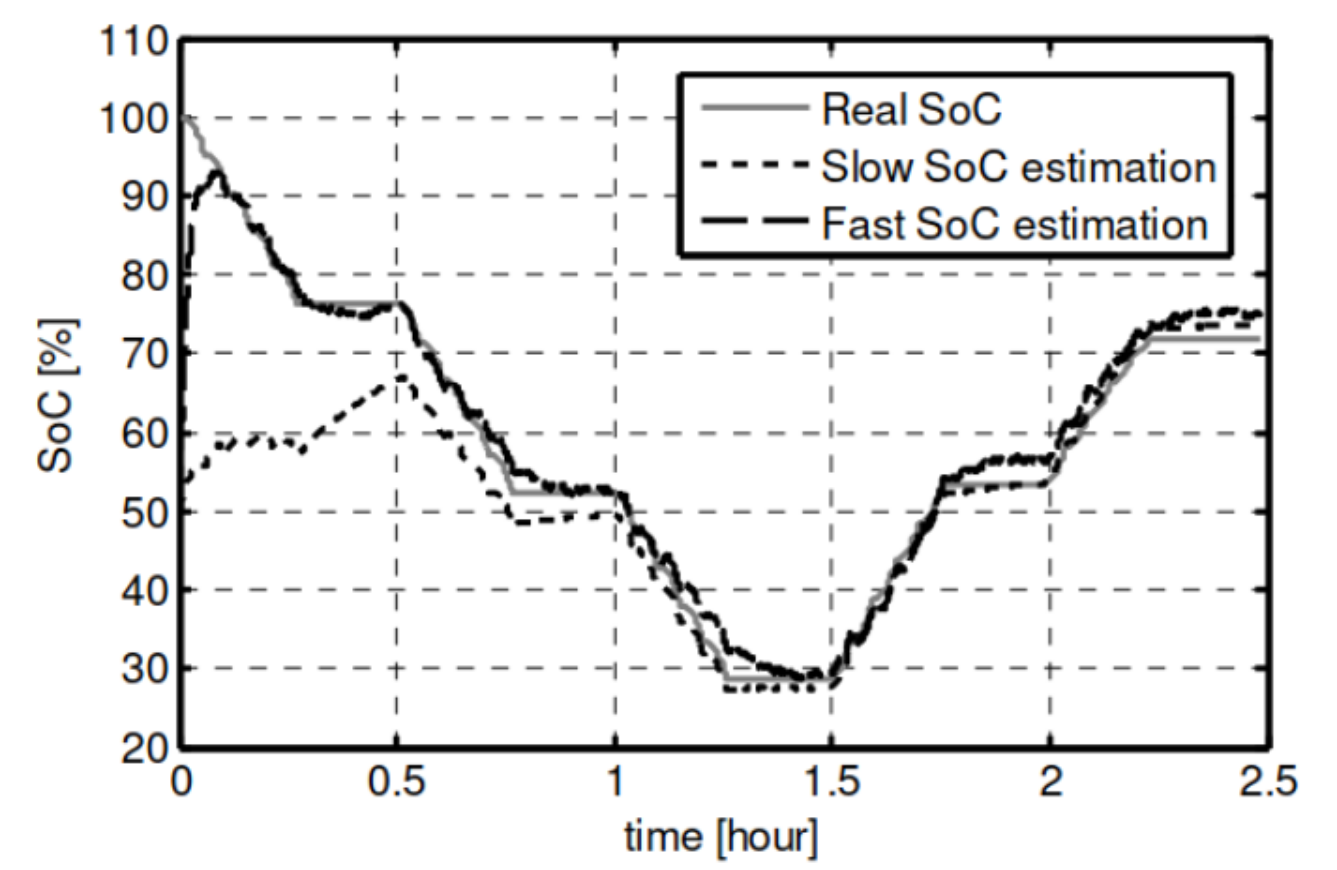
\includegraphics[width=0.7\textwidth]{soc_results_spagnoli.png}
        \caption{Resultados obtenidos en \cite{spagnol_kalman} sobre la
        estimaci\'on del Kalman con distintos par\'ametros de ajuste, con un
        \acrshort{SOC} inicial de un 50\%, se puede observar que la señal del
        \acrshort{SOC} converge a distintas velocidades al valor real.}
        \label{resultados_soc_spagnoli}
    \end{center}
\end{figure}

\noindent Los resultados de investigaciones relacionadas al Filtro de Kalman
como un observador del Estado de Carga obtuvieron resultados prometedores que
hacen que el algoritmo sea un gran candidato para sistemas en tiempo real, tales
como \acrshort{VVEE} o \acrshort{UPS}.

\subsubsection{M\'etodos basados en el aprendizaje autom\'atico}

\noindent El aprendizaje autom\'atico o, en ingl\'es, \acrfull{ML} surge como
una metodolog\'ia alternativa a la ingenier\'ia actual para el diseño de una
soluci\'on basado en un algoritmo. Como se ilustra en la Figura
\ref{curr_eng_approach}, el diagrama de flujo para el m\'etodo de ingenier\'ia
\emph{convencional} comienza con la \emph{adquisici\'on del conocimiento sobre
el tema}: El problema bajo estudio se analiza en detalle, produciendo un
\emph{modelo matem\'atico} que captura la \emph{f\'isica} del sistema,
identifica patrones de datos masivos y elaborar predicciones. Con este modelo,
se desarrolla un \emph{algoritmo optimizado} para el cálculo del \acrshort{SOC}
que ofrece determinado rendimiento asumiendo que el modelo f\'isico tiene un
cierto grado de exactitud en la representaci\'on de la realidad.

\begin{figure}[h!]
    \begin{center}
        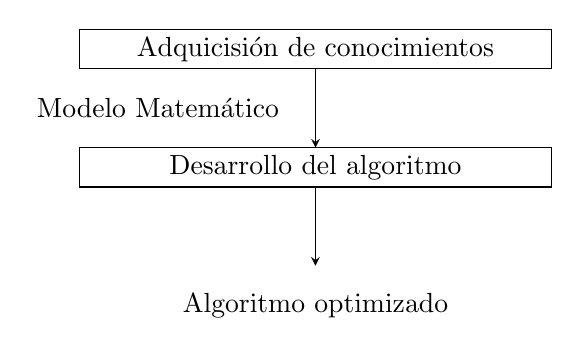
\begin{tikzpicture}
            \draw (0, 0) rectangle (6, -.5);
            \draw (3, -.25) node {Adquicisi\'on de conocimientos};
            \draw [-stealth] (3, -.5) -- (3, -1.5);
            \draw (1, -1) node {Modelo Matem\'atico};
            \draw (0, -1.5) rectangle (6, -2);
            \draw (3, -1.75) node {Desarrollo del algoritmo};
            \draw [-stealth] (3, -2) -- (3, -3);
            \draw (3, -3.5) node {Algoritmo optimizado};
        \end{tikzpicture}
    \end{center}
    \caption{Diagrama de flujo convencional para el desarrollo de algoritmos}
    \label{curr_eng_approach}
\end{figure}

\noindent Por su contraparte, y en su forma m\'as b\'asica, el m\'etodo por
aprendizaje autom\'atico substituye el paso de la adquisici\'on del conocimiento
previo con la tarea de recoleccionar un gran conjunto de datos (o, en ingl\'es,
\emph{dataset}) con un comportamiento espec\'ifico del sistema a modelar. Este
conjunto de datos se lo denomina \emph{set de entrenamiento}. Como se puede
observar en la Figura \ref{ml_approach}, el set de datos sirve como información
de entrada del algoritmo de aprendizaje que, como resultado, producirá una
\emph{m\'aquina} entrenada para llevar adelante la tarea deseada. En nuestro
caso el cálculo del \acrshort{SOC} del pack de batería. El aprendizaje es
realizado a trav\'es de un conjunto de algoritmos, tambi\'en conocidos como
\emph{hip\'otesis}, a partir de la toma la decisi\'ones ante estímulos obtenídos
del dataset. Los algoritmos de aprendizaje est\'an generalmente basados en la
optimizaci\'on de un criterio que mide cuan bien se desempeña el algoritmo de
aprendizaje seleccionado para la tarea a la que fue diseñado.

\begin{figure}[h!]
    \begin{center}
        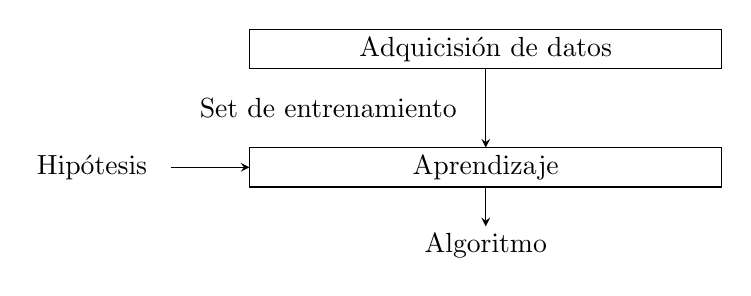
\begin{tikzpicture}
            \draw (0, 0) rectangle (6, -.5);
            \draw (3, -.25) node {Adquicisi\'on de datos};
            \draw [-stealth] (3, -.5) -- (3, -1.5);
            \draw (1, -1) node {Set de entrenamiento};
            \draw (0, -1.5) rectangle (6, -2);
            \draw (3, -1.75) node {Aprendizaje};
            \draw [-stealth] (3, -2) -- (3, -2.5);
            \draw (3, -2.75) node {Algoritmo};
            \draw [-stealth](-1, -1.75) -- (0, -1.75);
            \draw (-2, -1.75) node {Hip\'otesis};
        \end{tikzpicture}
    \end{center}
    \caption{Diagrama de flujo b\'asico para la generaci\'on de un modelo
    utilizando aprendizaje autom\'atico}
    \label{ml_approach}
\end{figure}

T\'ecnicas m\'as avanzadas del aprendizaje autom\'atico integran conocimientos
disponibles sobre el problema dentro del proceso de aprendizaje para lograr un
algoritmo m\'as robusto, esto suele ser aplicado, por ejemplo, en aplicaciones
para el procesamiento de im\'agenes donde el conocimiento sobre la invarianza
translacional de las caracter\'isticas visuales son utilizadas para adoptar
redes neuronales convolucionales (\acrshort{CNN}, del ingl\'es 
\emph{\acrlong{CNN}}) como hip\'otesis para ser entrenadas. Generalmente, como
se muestra en la Figura \ref{ml_ext_approach}, el conocimiento previo al
problema puede dictar la elecci\'on de hip\'otesis espec\'ificas para el uso
durante el proceso de entrenamiento. 

\begin{figure}[h!]
    \begin{center}
        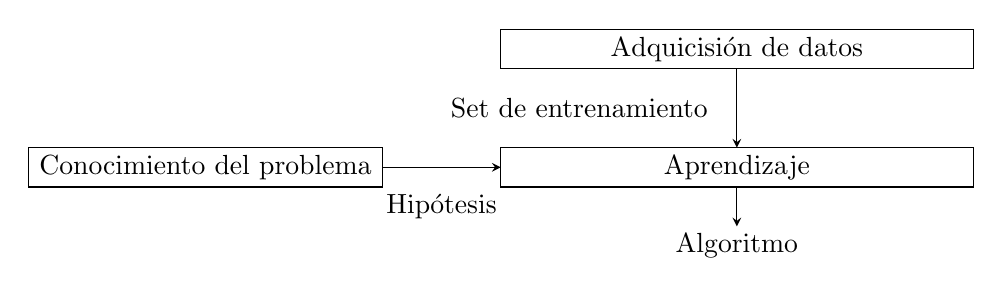
\begin{tikzpicture}
            \draw (0, 0) rectangle (6, -.5);
            \draw (3, -.25) node {Adquicisi\'on de datos};
            \draw [-stealth] (3, -.5) -- (3, -1.5);
            \draw (1, -1) node {Set de entrenamiento};
            \draw (0, -1.5) rectangle (6, -2);
            \draw (3, -1.75) node {Aprendizaje};
            \draw [-stealth] (3, -2) -- (3, -2.5);
            \draw (3, -2.75) node {Algoritmo};
            \draw [-stealth](-1.5, -1.75) -- (0, -1.75);
            \draw (-0.75, -2.25) node {Hip\'otesis};
            \draw (-6, -1.5) rectangle (-1.5, -2);
            \draw (-3.75, -1.75) node {Conocimiento del problema};
        \end{tikzpicture}
    \end{center}
    \caption{Diagrama de flujo para la generaci\'on de un algoritmo 
    utilizando aprendizaje autom\'atico y conocimientos del problema}
    \label{ml_ext_approach}
\end{figure}
\FloatBarrier

\noindent Dentro de la literatura que utiliza algoritmos de aprendizaje
autom\'atico para la estimaci\'on del \acrshort{SOC}, se propone el uso de
varias hip\'otesis detalladas a continuaci\'on,

\subsubsubsection{Redes Neuronales Artificiales}

\noindent Las redes neuronales artificiales (\acrshort{ANN}, del ingl\'es
\emph{\acrlong{ANN}}) tienen la capacidad de aprendizaje y adaptaci\'on para
poder representar un modelo no-lineal de gran complejidad. Las \acrshort{ANN}
puede usar un set de datos de entrenamiento para estimar el \acrshort{SOC} sin
conocer informaci\'on sobre la estructura interna de la bater\'ia ni el
\acrshort{SOC} inicial. Generalmente, se requieren al menos tres capas para
formar el algoritmo, incluyendo la capa de entrada, una o m\'as capas ocultas y
la capa de salida. La estructura de una \acrshort{ANN} para estimar el
\acrshort{SOC} se puede observar en la Figura \ref{ann_soc_layers}.

\begin{figure}[h!]
    \begin{center}
        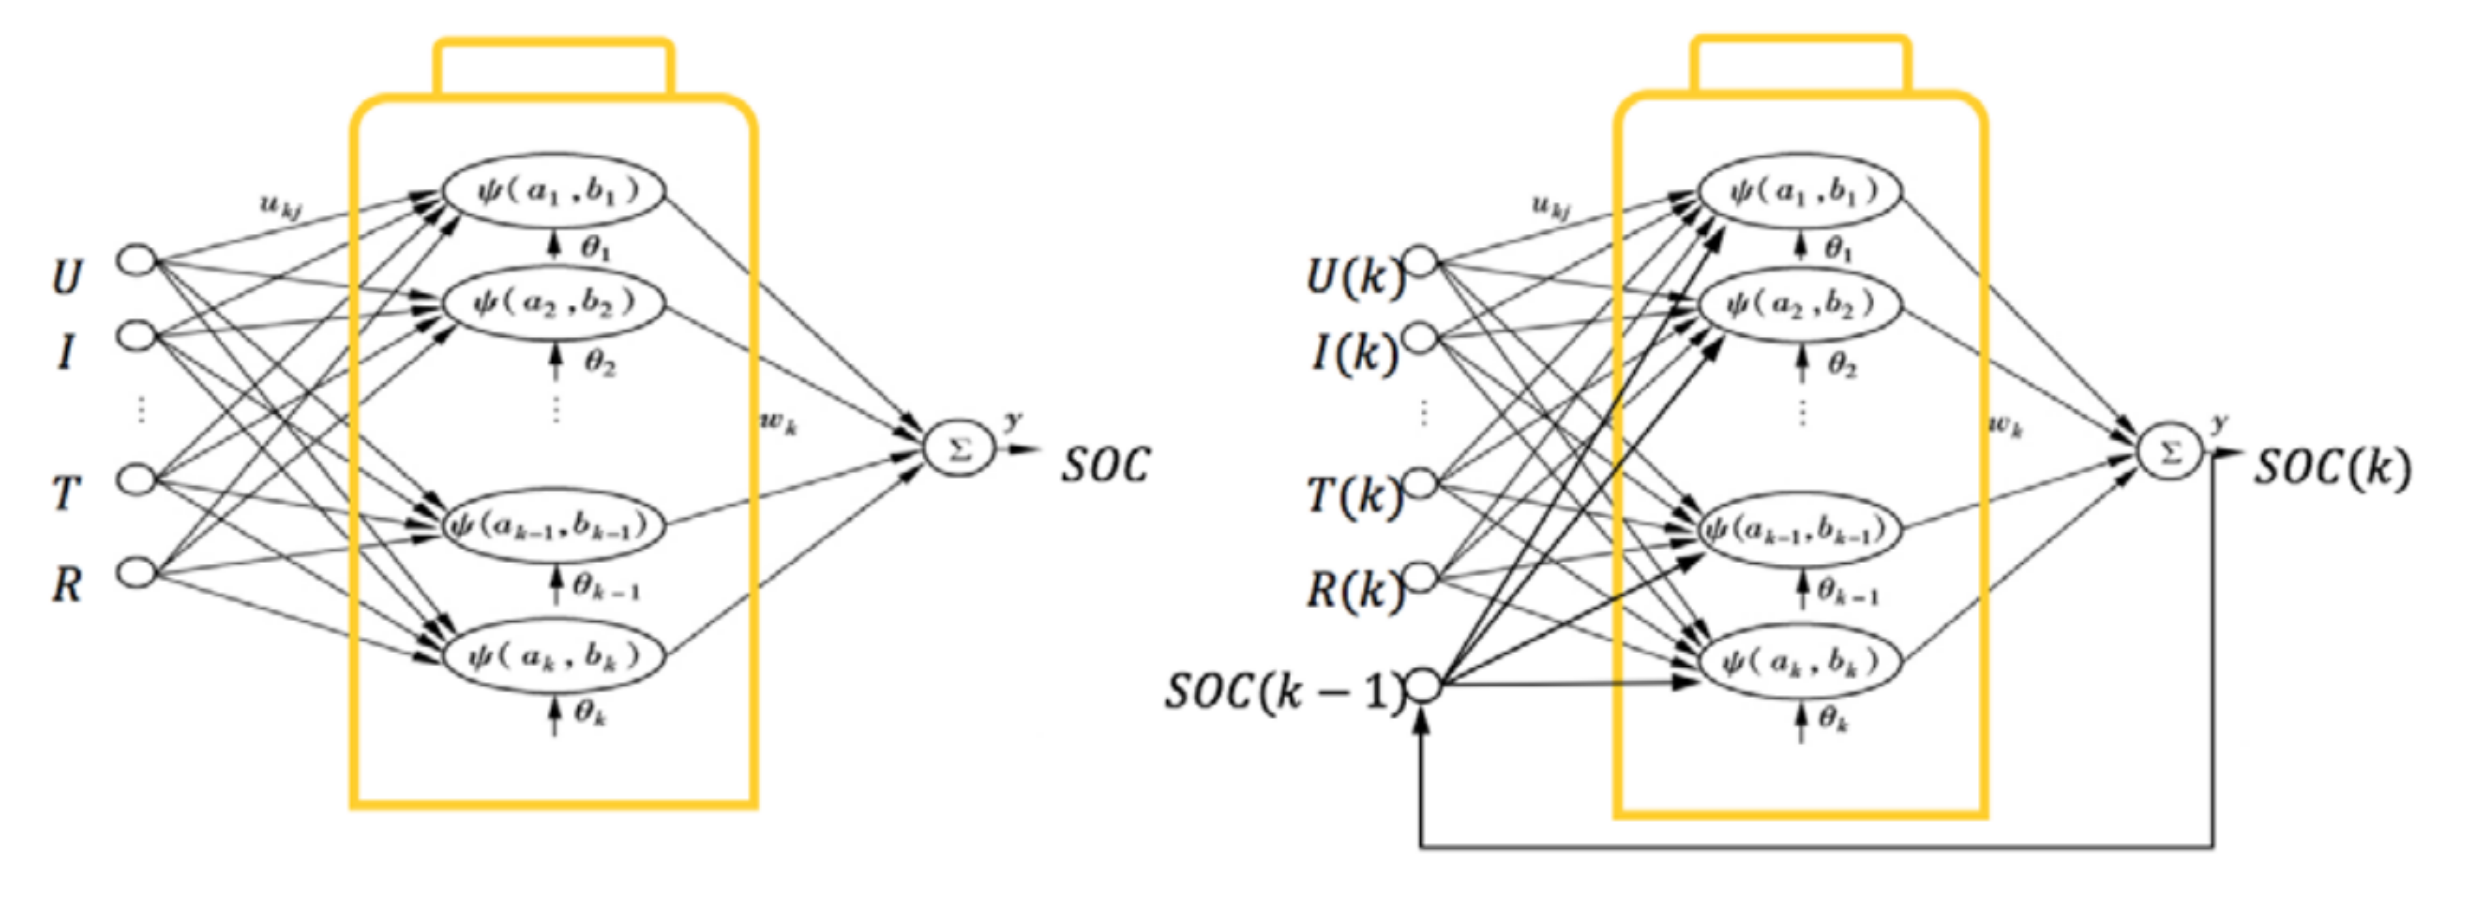
\includegraphics[width=1\textwidth]{ann_soc.png}
        \caption{Estrucutra de una \acrshort{ANN} para la estimaci\'on del
        \acrshort{SOC}}
        \label{ann_soc_layers}
    \end{center}
\end{figure}

\noindent \'Este m\'etodo utiliza el voltaje de la terminal, la corriente de
carga y descarga, y la temperatura ambiental como la entrada y la salida del
algoritmo es el \acrshort{SOC}. En \cite{XIA2018694} se propone el algoritmo
de Levenberg-Marquardt, una red neuronal optimizada basada en \emph{wavelets}.
En \cite{DANG2016356} se propone una red neuronal dual fusionada con un modelo 
de la bater\'ia para estimar el \acrshort{SOC}. Por el otro lado, 
\cite{TONG2016236} propone una nueva arquitectura para la estimaci\'on 
\acrshort{SOC} usando una red neuronal para clasificaci\'on de carga alcanzando 
un error de un 3.8\% en promedio. La gran ventaja de este m\'etodo es que puede 
operar bajo condiciones no-lineales obteniendo resultados \'optimos para su 
aplicaci\'on. Sin embargo, el algoritmo necesita un gran set de datos de 
entrenamiento, que no solo requiere gran poder computacional para poder 
entrenarlo, si no que tambi\'en un gran espacio de almacenamiento por lo cual su 
desarrollo es costoso si el presupuesto es limitado.

\newpage

\subsubsubsection{M\'aquinas de Vectores de Soporte}

\noindent El m\'etodo basado en las M\'aquinas de Vectores de Soporte 
(\acrshort{SVN} del ingl\'es \acrlong{SVN}) utiliza el algoritmo de regresi\'on 
lineal para transformar un modelo de baja dimensi\'on ($\mathrm{R^m}$) a otro de 
alta dimensi\'on ($\mathrm{R^n}$). \acrshort{SVM} fue diseñado, en principio, 
para  resolver problemas no-lineales de clasificaci\'on de dos clases. El punto 
clave de este m\'etodo es relacionar la muestra original del modelo de bajas 
dimensiones a uno de un espacio con mayores dimensiones encontrando un plano que 
puede separar ambas muestras de dos clases distintas, como se puede observar en 
la Figura \ref{svn_graph}

\begin{figure}[h!]
    \begin{center}
        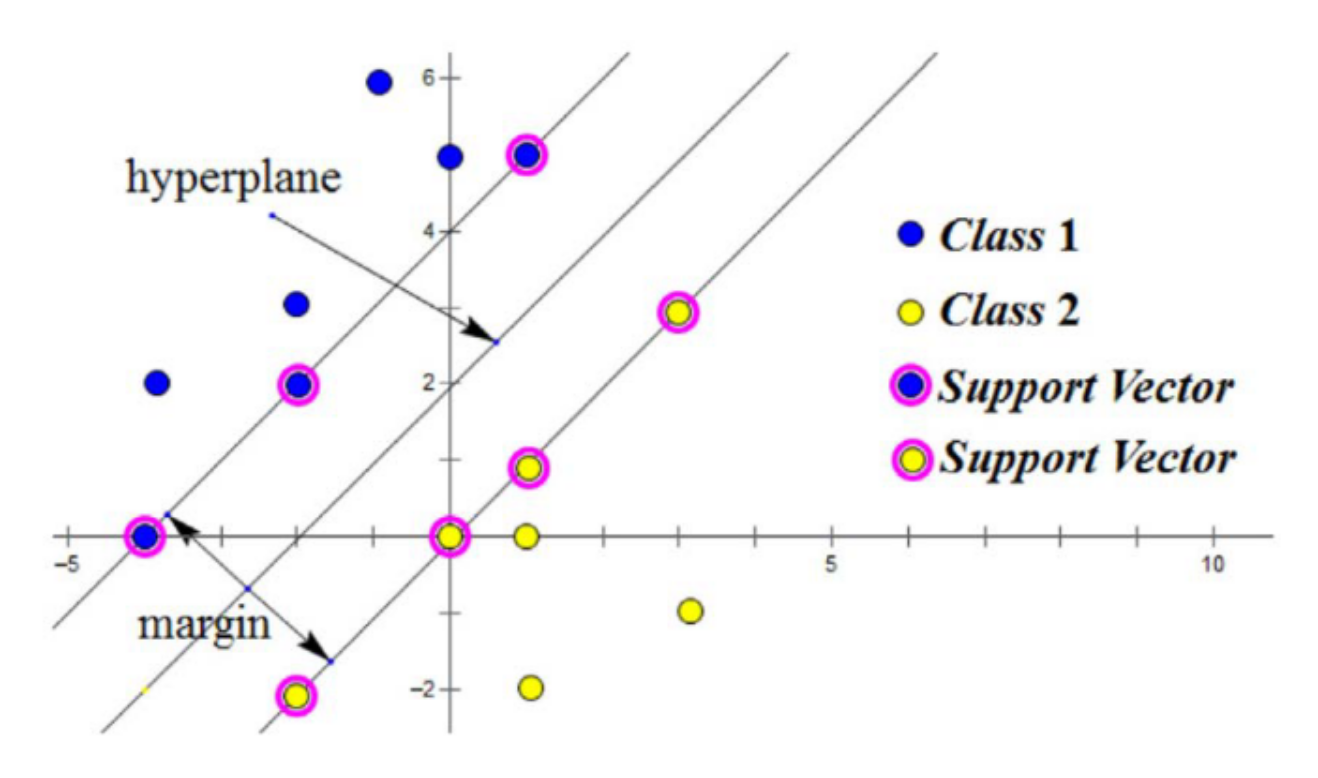
\includegraphics[width=.7\textwidth]{svm_graphic.png}
        \caption{Hiperplano que separa ambas clases}
        \label{svn_graph}
    \end{center}
\end{figure}

\noindent En \cite{HU2014682} se propone estimar el \acrshort{SOC} basado en 
\acrshort{SVM} optimizado para regresiones con un proceso de optimizaci\'on de 
doble b\'usqueda, utilizando

\noindent La arquitectura \acrshort{SVM}, tiene la habilidad de tolerar el ruido 
y escalar para integrar conocimientos de otros indicadores, tales como la 
temperatura, la energ\'ia entregada/consumida, entre otras variables de 
inter\'es. Sin embargo, este m\'etodo consume una gran cantidad de tiempo lo que 
lo imposibilita para funcionar en un sistema en tiempo real.

\subsubsubsection{L\'ogica Difusa}

\noindent La l\'ogica difusa (\acrshort{FL}, del ingl\'es \acrlong{FL}) es un
algoritmo utilizado para generar modelos complejos no-lineales con la ayuda de
un set de datos de entrenamiento. En este caso, \cite{DAI2015350} propone un 
algoritmo para la estimaci\'on del \acrshort{SOC} de forma \emph{online},
combinando un estimador cl\'asico del \acrshort{SOC} con un sistema fuzzy de
inferencia adaptativo (\acrshort{ANFIS}, del ingl\'es \acrlong{ANFIS}). \'Este
m\'etodo es propicio para adaptarse a distintas condiciones de operaci\'on de la
bater\'ia incluyendo el proceso de envejecimiento. La Figura \ref{anfis_arch}
ilustra una estructura b\'asica \acrshort{ANFIS} con cinco capas.

\begin{figure}[h!]
    \begin{center}
        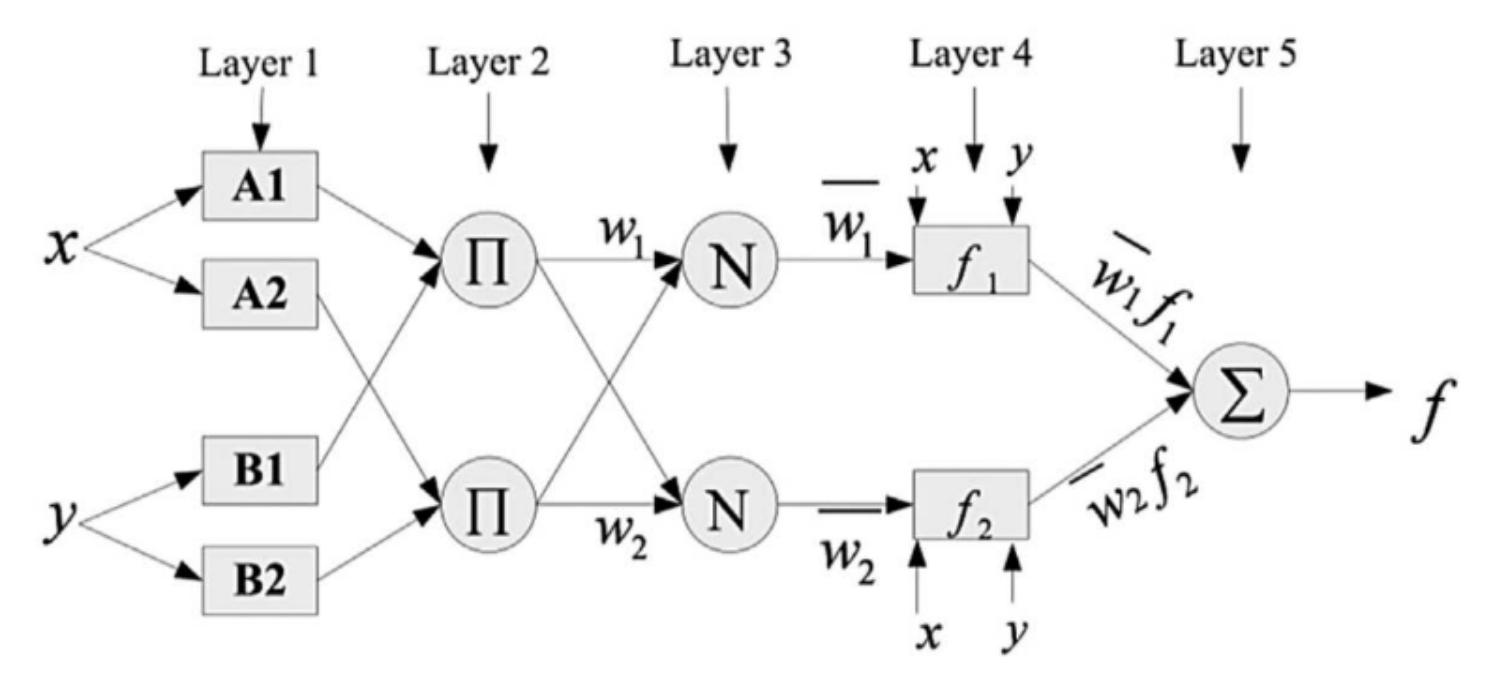
\includegraphics[width=0.8\textwidth]{anfis_arch.png}
        \caption{Arquitectura b\'asica para un \acrshort{ANFIS} de cinco capas}
        \label{anfis_arch}
    \end{center}
\end{figure}

\noindent A pesar de que la \acrshort{FL} tiene una poderosa habilidad para 
predicir modelos no lineales, la misma requiere algoritmos computacionales 
complejos y unidades de memorias de almacenamiento lo suficientemente amplios, 
logrando que el sistema sea excesivamente costoso para determinadas 
aplicaciones.

\newpage

\subsubsection{Algoritmo de Estimaci\'on}

\noindent La Figura \ref{comp_error_soc} demuestra la complejidad computacional 
en base al error en la estimaci\'on sobre los m\'etodos de estimaci\'on de 
\acrshort{SOC}.

\noindent En el presente, la estimaci\'on con mayor potencial y usado
ampliamente dentro de los \acrshort{BMS} es la combinaci\'on entre el modelo
el\'ectrico equivalente y un filtro de Kalman. El error m\'as significativo de
este m\'etodo proviene de los sensores de voltaje y corriente y no de la
influencia de los efectos intr\'insecos de la bater\'ia, como por ejemplo, el
envejecimiento, la temperatura y el efecto de hist\'erisis.

\begin{figure}[h!]
    \begin{center}
        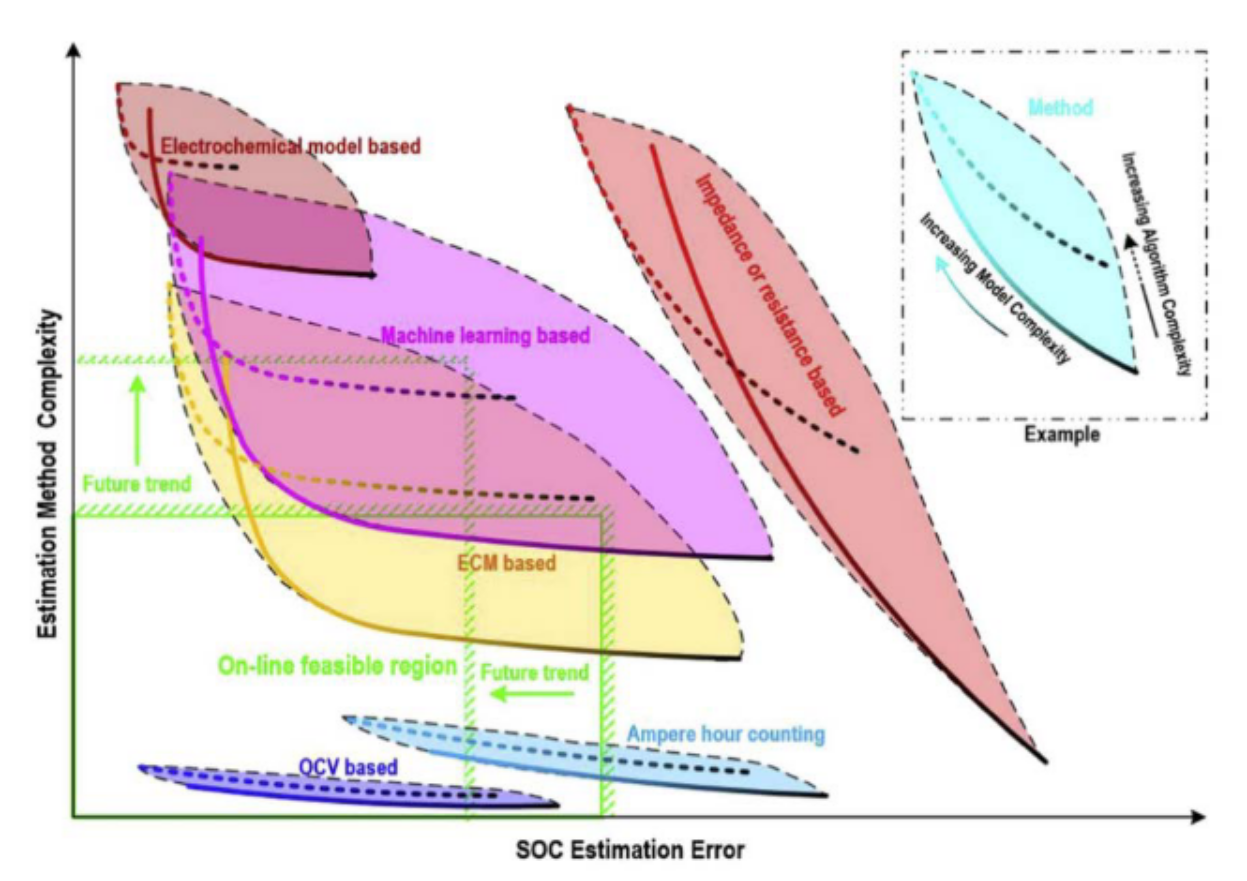
\includegraphics[width=0.8\textwidth]{comparisson_soc.png}
        \caption{Gr\'afica comparando los m\'etodos en base a la complejidad y
        exactitud}
        \label{comp_error_soc}
    \end{center}
\end{figure}

\subsection{Proceso de Carga}\label{sec:tecnica_carga}

El proceso de carga de una \acrfull{Ion-Li} no es trivial. Aplicar una tensión
constante en  bornes, como podríamos proceder con baterías de plomo ácido, no es
el procedimiento más adecuado en este caso. En aras de optimizar la autonomía y
la vida útil del pack de baterías el proceso de carga debe responder a
lineamientos particulares de acuerdo a las carácterísticas constructivas de las
celdas que lo componen. Este proceso est\'a descripto por un perfil de Corriente
Constante (CC) - Voltaje Constante (CV)

\subsubsection{Corriente Constante CC - Voltaje Constante CV}

El perfil de carga que se ajusta a las celdas de \acrshort{Ion-Li}, como se
observa en la figura \ref{fig:char_prof}, es el perfil \acrshort{CC} -
\acrshort{CV}. Este consiste en tres fases, una primera etapa de
acondicionamiento o pre carga donde se inyecta a la batería una corriente
constante pequeña de magnitud equivalente a la corriente de fin de carga. Una
fase de carga rápida a corriente constante \acrshort{CC} y una tercer y última
fase de carga a tensión constante \acrshort{CV}.

\begin{figure}[h!] \centering
    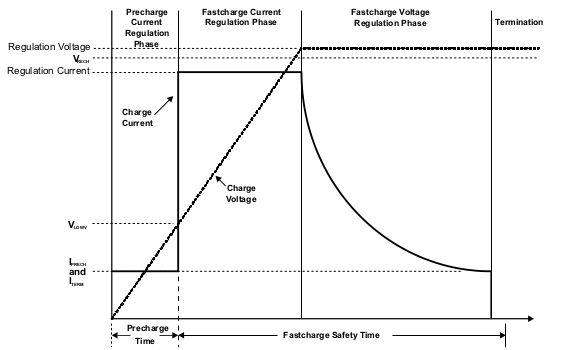
\includegraphics[width=0.8\textwidth]{bat_char/char_profile.png}
    \caption{Perfil de carga típico de una batería de Ion-Litio}
\label{fig:char_prof} \end{figure} \FloatBarrier

El proceso de pre-carga o pre-acondicionamiento proporciona a las celdas la
capacidad de recuperar su capa de pasivación, la cual puede haberse visto
afectada o disuelta tras largos per\'iodos de almacenamiento en estados de
descarga profunda. A su vez permite introducir las celdas en la zona de
operación segura en caso de que se encuente profundamente descargadas. Es
importante limitar el proceso de acondicionamiento en tiempo para prevenir 
pre-cargar indefinidamente una celda que se encuentre agotada. Si tras un 
periodo completo de acondicionamiendo la celda no alcanza el voltaje mínimo 
necesario puede considerarse que la misma alcanzó el final de su vida útil.

El voltaje umbral de inicio de carga rápida depende de la composici\'on
qu\'imica de la celda y en el caso de las baterías litio-ion, la misma 
se ubica generalmente entre los 2.5V y 3.0V. Una vez que la celda supera su 
voltaje umbral mínimo el cargador deber\'a entrar en la zona de carga rápida, es
decir, en la etapa de corriente constante \acrshort{CC}. La fase de carga rápida 
permite a la batería transformar la enería eléctrica entregada en energía 
electroquímica dentro de la batería en el menor tiempo posible. La magnitud de 
la corriente de carga rápida depende de la celda y es limitada generalmente 
entre 0.5C y 1C para prevenir el calentamiento del pack y su degradación 
prematura. El pack de batería admitirá carga rápida a corriente constante hasta 
alcanzar el voltaje límite de regulación. 

En esta tercer, y última fase, la corriente drenada del pack decae
exponencialmente hasta alcanzar la magnitud de fin de carga, situación que nos
indica que el ciclo se completo exitosamente. La corriente de terminación de
carga ronda entre 5\% y 10\% de la corriente de carga rápida. Cabe aclarar
que en esta instancia del proceso de carga la corriente decae naturalmente dado
que la magnitud controlada por el cargador es la tensi\'on en bornes de la
celda.  

Es importante remarcar que durante todo el proceso de carga, 
fundamentalmente durante la fase de carga rápida a corriente constante, es de
vital importancia monitorear la temperatura de las celdas evitando que las
mismas se aparten de la zona de operación segura, ya que el proceso de carga
implica intrínsicamente una elevación de la temperatura de la celda, entre otras
causas, debido a su resistencia interna.

El tiempo total de carga es una variable determinante a la hora de implementar
un cargador de batería que extienda al máximo la vida útil y los ciclos de carga
de un pack de baterías y de sus celdas. Es la magnitud de corriente de carga
rápida la variable determinante de este tiempo. Por ejemplo, para una
carga rápida a 1C, la batería alcanzará, durante la fasé de \acrshort{CC}, el
$70\%$ de su capacidad total en el $30\%$ del tiempo de carga mientras que
tardará el $70\%$ del tiempo total de carga para acumular el $30\%$ restante de
su capacidad durante la fase \acrshort{CV}. 

La existencia de una resistencia interna en serie en las celdas no ideales
implica que a mayor corriente de carga rápida a CC se alcance más rápido la
tensión de umbral de paso a la fase de tensión constante CV acortando el tiempo
de CC pero extendiendo el tiempo de CV. Podemos inferir entonces que a menor
resistencia interna menor tiempo de carga. Y que aumentar la corriente a CC
tambien reducirá el tiempo de carga.  Sin embargo, se desaconseja completamente
implementar regímenes de carga rápida que superen 1C por el impacto en el número
de ciclos de vida útil de las celdas del pack de batería. La figura
\ref{fig:C_vs_Cycle_I} muestra como a medida que aumentamos el régimen de carga
de una celda la vida \'util de la misma, medido en ciclos de carga, disminuye
significativamente.

\begin{figure}[h!] \centering
    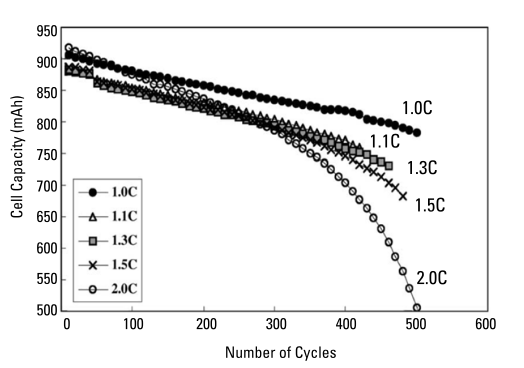
\includegraphics[width=0.6\textwidth]{bat_char/C_vs_Cycle_I.png}
    \caption{Relación Corriente de carga vs Ciclos de vidaútil de una celda de
    Ion-Litio con un cátodo de $LiCoO_2$} \label{fig:C_vs_Cycle_I} 
\end{figure}
\FloatBarrier

A mayores tasas de corriente, mayor cantidad de iones de litio se depositan
sobre el ánodo conviritiendose en litio metálico al librerar sus electrónes
disponibles.  El litio metálico es sumamente reactivo con el electrolito
resultando en una pérdida permanente de \acrshort{Ion-Li}, el elemento
almacendor de la energía, acelerando el envejecimiento prematuro de la celda y
en consecuencia reduciendo los ciclos de vida útiles de la misma. 

Normalmente, a mayor voltaje en bornes de una celda mayor es la capacidad de la
misma. Podríamos entonces vernos tentados a aumentar el voltaje límite de
regulación y sobre cargar una celda para aumentar la carga almacenada. Por
ejemplo, una celta cargada a $4.3V$ en vez de $4.2V$ va a permitirnos almacenar
un $10\%$ más de carga inicial. El inconveniente aqui reside nuevamente en el
impacto que tendra este procedimiento en el número de ciclos de carga y la vida
útil de la celda. La vida útil de una celda sobrecargada se vería reducida en
un $50\%$.  Por el otro lado, cargar una celda con un un voltaje menor ($40mv$
menor) implicará una reducción aproximada de un $10\%$ de su carga inicial.
Podemos arribar a la conclusión que el control del voltaje de carga y su
precisión es de vital importancia en un circuito de carga. La figura
\ref{fig:C_vs_Cycle_V} muestra la relación entre el número de ciclos de carga y
los diferentes voltajes de carga. 

\begin{figure}[h!] \centering
    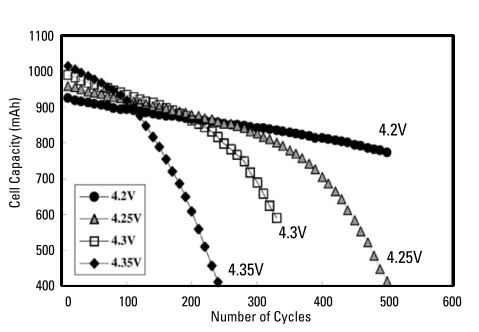
\includegraphics[width=0.6\textwidth]{bat_char/C_vs_Cycle_V.png}
    \caption{Relación Voltaje de carga la batería vs Ciclos de vida de una celda de
Ion-Litio con un cátodo de $LiCoO_2$} \label{fig:C_vs_Cycle_V} \end{figure}
\FloatBarrier

A voltajes mayores el material del cátodo reacciona a mayor velocidad con el
electrolito perdiéndose material en la reacción resultando en una perdida de
capacidad de almacenamiento de energía. Sumado al control del proceso de carga,
tambi\'en se debe monitorear sobre el mismo la ecualizaci\'on de las celdas en
caso de que el pack de bater\'ias posea una arquitectura con mayor cantidad de
celdas conectadas en serie.

\subsection{Ecualización de celdas}\label{cell_balancing_theory}

Los packs de bater\'ias en los \acrshort{VVEE} consisten de un gran n\'umero de
celdas agrupadas en serie y en paralelo para proveer la suficiente energia y
potencia al veh\'iculo. Sin embargo, las caracter\'isticas internas de la
bater\'ia incluyendo capacidad inicial, impedancia interna, volumen f\'isico,
corriente de auto-descarga, etc., y condiciones externas, tales como la
temperatura ambiental, son siempre inconsistentes en la vida real. Al nivel del
pack de bater\'ias, las variaciones de par\'ametros entre celdas en serie puede
llevar a una degradaci\'on acelerada del mismo, con un impacto negativo en la
potencia, capacidad, tiempo de vida restante, entre otras limitaciones. El
desbalance puede deteriorar este degradamiento al punto de poner en riesgo al
veh\'iculo desencadenando un embalamiento t\'ermico del pack. Por lo tanto, la
ecualizaci\'on del pack de bater\'ias, que puede mejorar la seguridad y
rendimiento del mismo es una tecnolog\'ia cr\'itica dentro del \acrshort{BMS}
para la reducci\'on del desbalance entre celdas.

La ecualizaci\'on tambi\'en es cr\'itica para un segundo uso de celdas de
litio-ion que se encuentra en desuso. Las bater\'ias con una capacidad degradada
en un 20\% deber\'ian ser reemplazadas para garantizar seguridad y autonom\'ia
al \acrshort{VE}. Reacondicionando celdas en desuso para bicicletas
el\'ectricas, veh\'iculos el\'ectricos de excursi\'on y sistemas de
almacenamiento de energ\'ia, pueden generar beneficios tanto ambientales como
econ\'omicos, y esto es posible gracias a una eficiente ecualizaci\'on de las
celdas.

Los circuitos de ecualizaci\'on, o \emph{ecualizadores}, combinados con
estrategias de ecualizaci\'on pueden ayudar evitar el problema del desbalanceo
dentro del pack de bater\'ias. A pesar de que distintas aplicaciones de
\acrshort{VE} tienen distintos requerimientos, la topolog\'ia del diseño del
hardware est\'a limitado por el costo, tamaño y fiabilidad. A pesar del progreso
dentro de esta tecnolog\'ia, las soluciones existentes no puede resolver todos
los requerimientos de estos sistemas. Por lo tanto, es esencial primero
describir los motivos de las inconsistencias entre celdas y el estado de arte de
la tecnolog\'ia actual para el diseño del \acrshort{BMS}

\newpage

\subsubsection{Inconsistencias entre celdas}

Para satisfacer la demanda de voltaje, potencia y energ\'ia en los 
\acrshort{VVEE}, los packs de bater\'ia contienen desde decenas hasta miles de
celdas conectadas en serie o en paralelo y, las inconsistencias entre ellas son
inevitables por una gran cantidad de motivos. Uno de los primeros problemas que
traen estas inconsistencias es que la capacidad del pack de bater\'ias est\'a
limitado por la celda de menor capacidad, este defecto tienen un nombre y es el
\emph{efecto barril}, el mismo se puede visualizar en la Figura 
\ref{barrel_effect}A, en este caso el pack de bater\'ias cesar\'a la descarga del
pack si cualquiera de las celdas alcanza el fin de la descarga. De forma
similar, la carga disponible del pack de bater\'ias, como se puede observar en
la Figura \ref{barrel_effect}B, est\'a limitado por la celda con menor
capacidad, donde el pack finalizar\'a el proceso de carga si cualquiera de las
celdas alcanza el final de carga. Por lo tanto, la capacidad de carga/descarga
del pack est\'a fuertemente influenciado por estas inconsistencias.

Sumado a eso, estas inconsistencias son variantes en el tiempo y asociadas a
varios factores, especialmente con la degradaci\'on del pack. Las
caracter\'isticas no lineales del envejecimiento de las celdas de litio-ion
afectar\'an gradualmente la inconsistencia del pack. A pesar de que las celdas
pueden tener un desapareamiento de capacidad inicial de un 3\%, esta
inconsistencia no puede ser eliminada y tiene una tendencia a empeorar llevando
a una degradaci\'on prematura y aumentar los riesgos de sobrecarga/descarga
durante cada ciclo llegando finalmente a un embalamiento t\'ermico.

Los or\'igenes de las inconsistencias pueden ser separados en dos grupos: el
proceso de producci\'on y el uso de las mismas. El primero puede ser causado por
variaciones en los materiales, equipo de producci\'on y procedimientos, que
llevan a una inconsistencia en los par\'ametros entre celdas del mismo modelo.
Mientras que el segundo est\'a fuertemente relacionado con las diferencias
ambientales durante el uso y almacenamiento de las bater\'ias. Ambas
inconsistencias influyen directamente sobre el rendimiento del pack de
bater\'ias.


\begin{figure}[h!]
    \begin{center}
        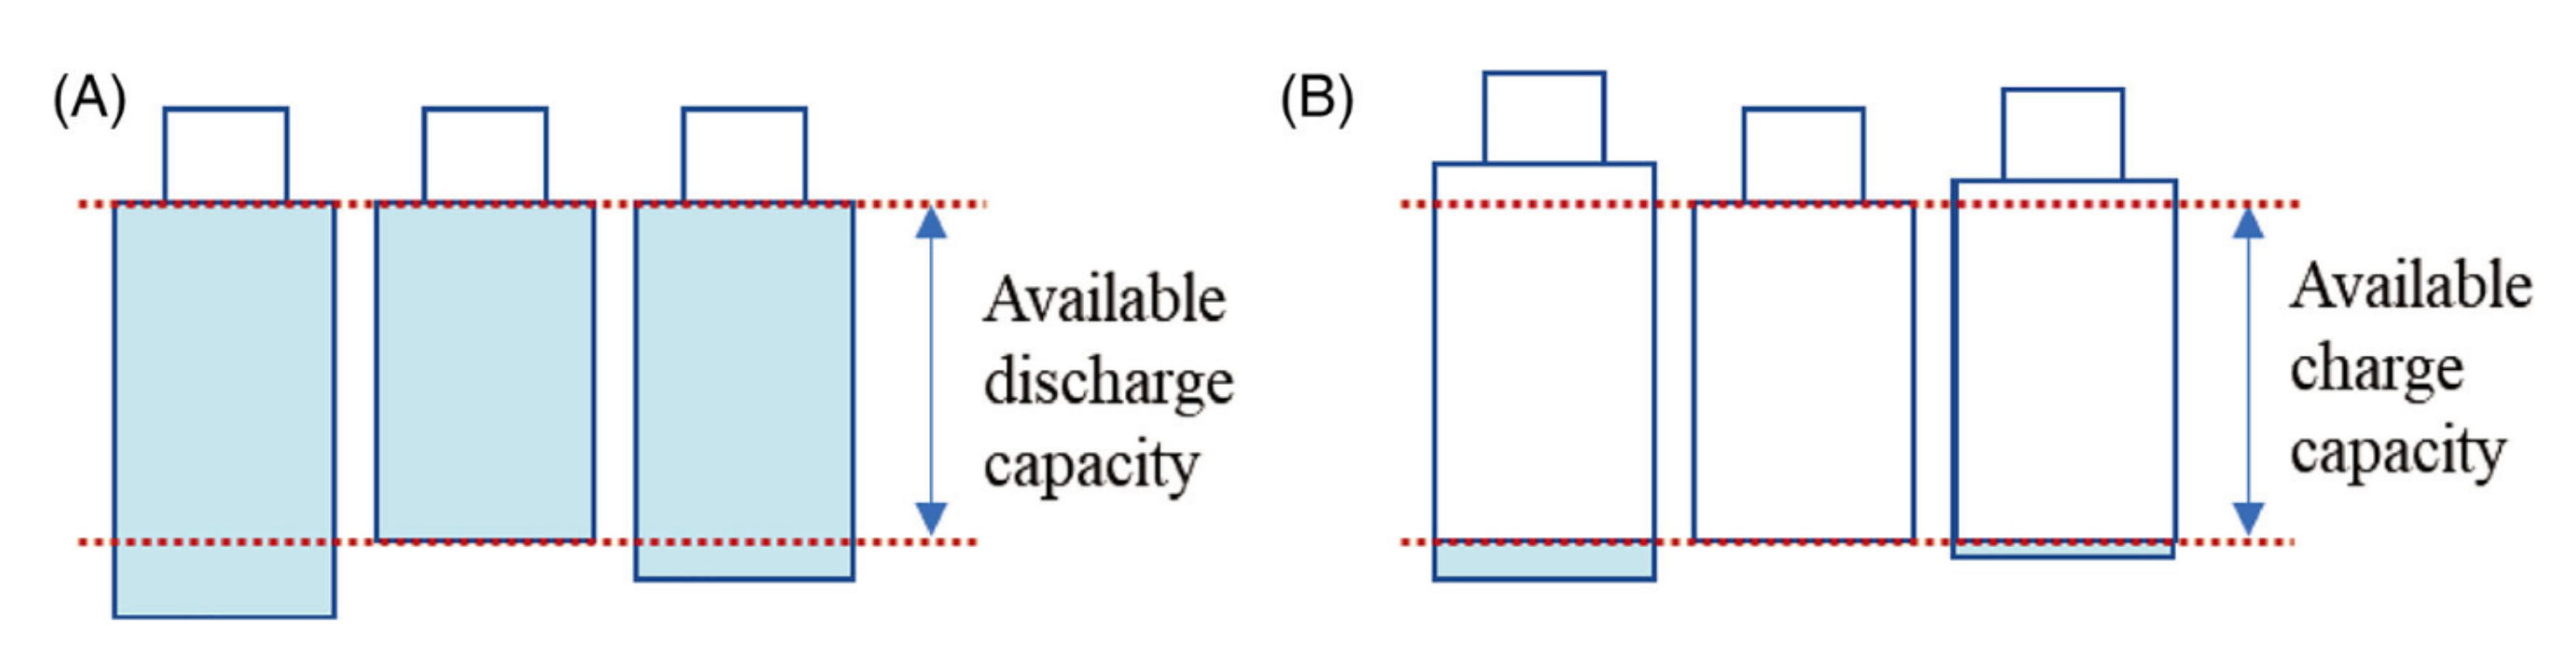
\includegraphics[width=1\textwidth]{barrel_effect.png}
        \caption{(A) Capacidad de descarga disponible. (B) Capacidad de carga
        disponible}
        \label{barrel_effect}
    \end{center}
\end{figure}

\subsubsubsection{Inconsistencias causadas por la producci\'on}

El proceso de producci\'on de las celdas de litio-ion consiste en mezclar
materiales acuosos, cubrir, cortar, devanar, ensamblar e inyectar electrolito,
donde cada paso puede provocar variaciones y afectar la inconsistencia en la
producci\'on de los distintos lote. Por ejemplo, la mezcla no uniforme de las
sustancias puede provocar defectos sutiles en la microestructura de la celda,
que afecta de forma directa al rendimiento de las mismas. Debido a las
diferencias en el material, precisi\'on en los equipos y la incerteza del
proceso de producci\'on, las diferencias entre baches de producci\'on son
inevitables. La otra influencia de heterogeneidad inicial incluye a la capacidad
inicial y a la resistencia interna, concentraci\'on de litio-ion, grosor del
separador entre otros.

Las inconsistencias causadas por el proceso de producci\'on no pueden ser
eliminadas por completo. Sin embargo, se pueden utilizar m\'etodos de
apareamiento a la hora de ensamblar el pack de bater\'ias para combinar aquellas
que sean consistentes entre s\'i, mejorando la fiabilidad, seguridad y tiempo de
vida de un pack de bater\'ias. \'Estos m\'etodos se basan en criterios tales
como la capacidad, la resistencia interna y la corriente de auto-descarga.

\subsubsubsection{Inconsistencias causadas por el ensamblaje del pack}

Adem\'as del proceso de producci\'on, la tecnolog\'ia de ensamblado de los
packs de bater\'ias tambi\'en son esenciales para mantener la consistencia de
los par\'ametros. Por ejemplo, el grado de ajuste afectar\'a el estr\'es
mec\'anico impuesto sobre las celdas, y el espacio entre bater\'ias puede
afectar la disipaci\'on del calor generado por la corriente de carga/descarga.
En \cite{JI2019113683} se estudia el efecto la uniformidad del espacio entre 
celdas. Los resultados muestran un modelo t\'ermico-electroqu\'imico acoplado que 
ilustra como la variaci\'on del espacio puede mejorar la homogeneidad entre 
celdas modelo 18650, y concluye en que la temperatura puede reducirse en un 13\% 
cuando el espacio es modificado de 3mm a 5.5mm.

La distribuci\'on de temperatura puede influir ampliamente en la inconsistencia
de la bater\'ia, que se encuentra directamente relacionado con el diseño del
ensamblado. Las bater\'ias pueden generar calor durante su uso, que no puede
disiparse instant\'aneamente incrementando as\'i la temperatura de la bater\'ia.
Adicionalmente, el intercambio de calor con el ambiente de la bater\'ia
tambi\'en es diferente, por ejemplo, las bater\'ias externas tiene una gran
superficie de intercambio de calor, mientras que las bater\'ias encapsuladas
internamente pueden intercambiar calor solamente con las bater\'ias adyacentes.
Por lo tanto, el diseño del ensamblaje puede llevar a diferentes distribuciones
de temperatura, logrando una inconsistencia entre celdas.

\subsubsubsection{Inconsistencias causadas por el uso}

Las celdas en el mismo pack tienden a mantener la uniformidad despu\'es del
ensamblaje inicial, pero la inconsistencia de este ensamblaje puede incrementar
gradualmente, ya sea por el almacenamiento de la bater\'ia o el uso, reduciendo
el rendimiento del pack. El estr\'es f\'isico y qu\'imico puede acumularse
de forma gradual durante el uso de la bater\'ia. El proceso de degradaci\'on es
muy complicado, incluyendo varios mecanismos de envejecimiento y sus
interacciones dentro de las bater\'ias, y la degradaci\'on de los electrodos es
el factor principal que causa el decaimiento en el rendimiento de la bater\'ia.
Factores tales como la temperatura, corriente, \acrshort{SOC} pueden afectar
significativamente los materiales activos y las microestructuras, y la
variaci\'on entre estos factores inevitablemente afectar\'a de forma negativa
las inconsistencias dentro del pack.

La temperatura es un factor cr\'itico de envejecimiento que afecta la velocidad
de degradaci\'on. La diferencia de temperatura causar\'a que las celdas
envejezcan a distinta velocidad, agravando las inconsistencias dentro del pack
de bater\'ias. Tanto altas como bajas temperaturas aceleran este proceso.
Trabajando o almacenando en altas temperaturas pueden aceleras las reacciones
secundarias, y cargar a bajas temperaturas puede resultar en el dep\'osito de
litio s\'olido y el crecimiento de dendritas dentro del material activo.
Adem\'as, las diferencias en la resistencia interna y la capacidad cal\'orica
entre celdas puede resultar en una distribuci\'on heterog\'enea dentro del pack.
Acoplado con convecci\'on forzada y un canal de enfriamiento, la disipaci\'on de
calor uniforme incrementa la diferencia en la degradaci\'on entre celdas
afectando el tiempo de vida y la capacidad disponible de ellas. 

La circulaci\'on de altas corrientes desde y hacia el pack puede incrementar el
proceso de difusi\'on inducido poniendo a las bater\'ias bajo estr\'es, 
acelerando el proceso de envejecimiento. Adicionalmente, la diferencia
de corriente entre bater\'ias puede causar variaciones en temperatura entre
ellas, por lo tanto, como se menciona anteriormente, empeorando las
inconsistencias entre el pack. Para las bater\'ias conectadas en paralelo donde
el voltaje entre celdas es el mismo, se pueden encontrar pequeñas diferencias
debido a la resistencia en el cable y los puntos de soldadura hasta en la
posici\'on de las bater\'ias. Por el otro lado, para las celdas en serie, la
corriente que circula a trav\'es de ellas es siempre la misma, a pesar de ello,
el estr\'es sobre los m\'odulos de menor capacidad es mayor, haciendo que su
capacidad disminuya r\'apidamente, como consecuencia de esto, se forma un
proceso de realimentaci\'on positiva, ya que al disminuir la capacidad de estas
celdas, su resistencia interna aumenta por lo que aumenta la temperatura de las
mismas llegando a una instancia de riesgo t\'ermico.

Por \'ultimo, el \acrshort{SOC} es otro factor de estr\'es importante. Un
\acrshort{SOC} alto o una sobrecarga significa menos potencial en el \'anodo,
que desencadena reacciones secundarias, descomposici\'on del electrolito y una
mayor posibilidad de que se forme litio met\'alico alrededor del \'anodo 
durante el proceso de carga, mientras que un \acrshort{SOC} puede llevar a la 
corrosi\'on del cobre en el colector del \'anodo u desordenar la estructura del 
material en el c\'atodo. Diferencias de \acrshort{SOC} entre celdas puede llevar 
a velocidades de envejecimiento inconsistente, causando tambi\'en una diferencia 
entre el \acrshort{DOD}.

\subsubsubsection{Administraci\'on de la inconsistencia}

La inconsistencia en el pack no puede ser completamente eliminada pero puede ser
restringida a un rango de operaci\'on razonable. Para resolver esto existe un gran
espectro de m\'etodos a aplicar.

Las inconsistencias generadas por los procesos de manufactura y ensamble pueden
ser atenuados mejorando la estabilidad y consistencia de los materiales
utilizados (como por ejemplo, el material del c\'atodo, \'anodo, electrolito,
etc) y mejorando la uniformidad de los procesos de producci\'on. El apareamiento
de las celdas previo al ensamblado tambi\'en influye en la mejora de las
inconsistencias del pack de bater\'ias.

Una vez ensamblado, la consistencia de las celdas disminuir\'a durante el uso de
las mismas y puede llevar a serios desperfectos si no es administrado de manera
correcta. La consistencia entre celdas puede ser mejorada a trav\'es de varios
mecanismos, como por ejemplo, estructuras mec\'anicas apropiadas o el proceso de 
ecualizaci\'on en el \acrshort{BMS}.

\subsubsection{Sistema de Administraci\'on de Ecualizaci\'on}

El sistema de administraci\'on de ecualizaci\'on (\acrshort{EMS}, del ingl\'es
\emph{\acrlong{EMS}}) juega un papel importante en la reducci\'on de
inconsistencias entre las celdas del pack. Existe una gran variedad de
t\'ecnicas de ecualizaci\'on que fueron investigadas e implementadas en
\acrshort{VVEE}.

\subsubsubsection{Clasificaciones}

Los \acrshort{EMS} pueden ser clasificados entre sistemas pasivos y activos
dependiendo de la topolog\'ia del circuito. Independientemente de la
topolog\'ia, la bater\'ia a balancear debe ser seleccionada seg\'un un criterio
espec\'ifico, que usualmente se basa en las caracter\'isticas de la misma, como
la tensi\'on de los terminales, \acrshort{SOC} o capacidad, que son consideradas
variables de balanceo. Dependiendo de las variables espec\'ificas, los 
\acrshort{EMS} pueden ser clasificados en ecualizaci\'on basada en voltaje, 
capacidad o \acrshort{SOC}. Dependiendo de la estrategia de control de balanceo,
los \acrshort{EMS} pueden ser divididos entre control cl\'asico, control de 
l\'ogica difusa, control predictivo y otros m\'etodos avanzados. La t\'ipica
clasificaci\'on de los \acrshort{EMS} se puede visualizar en la Figura
\ref{ems_classes}.

\begin{figure}[h!]
    \begin{center}
        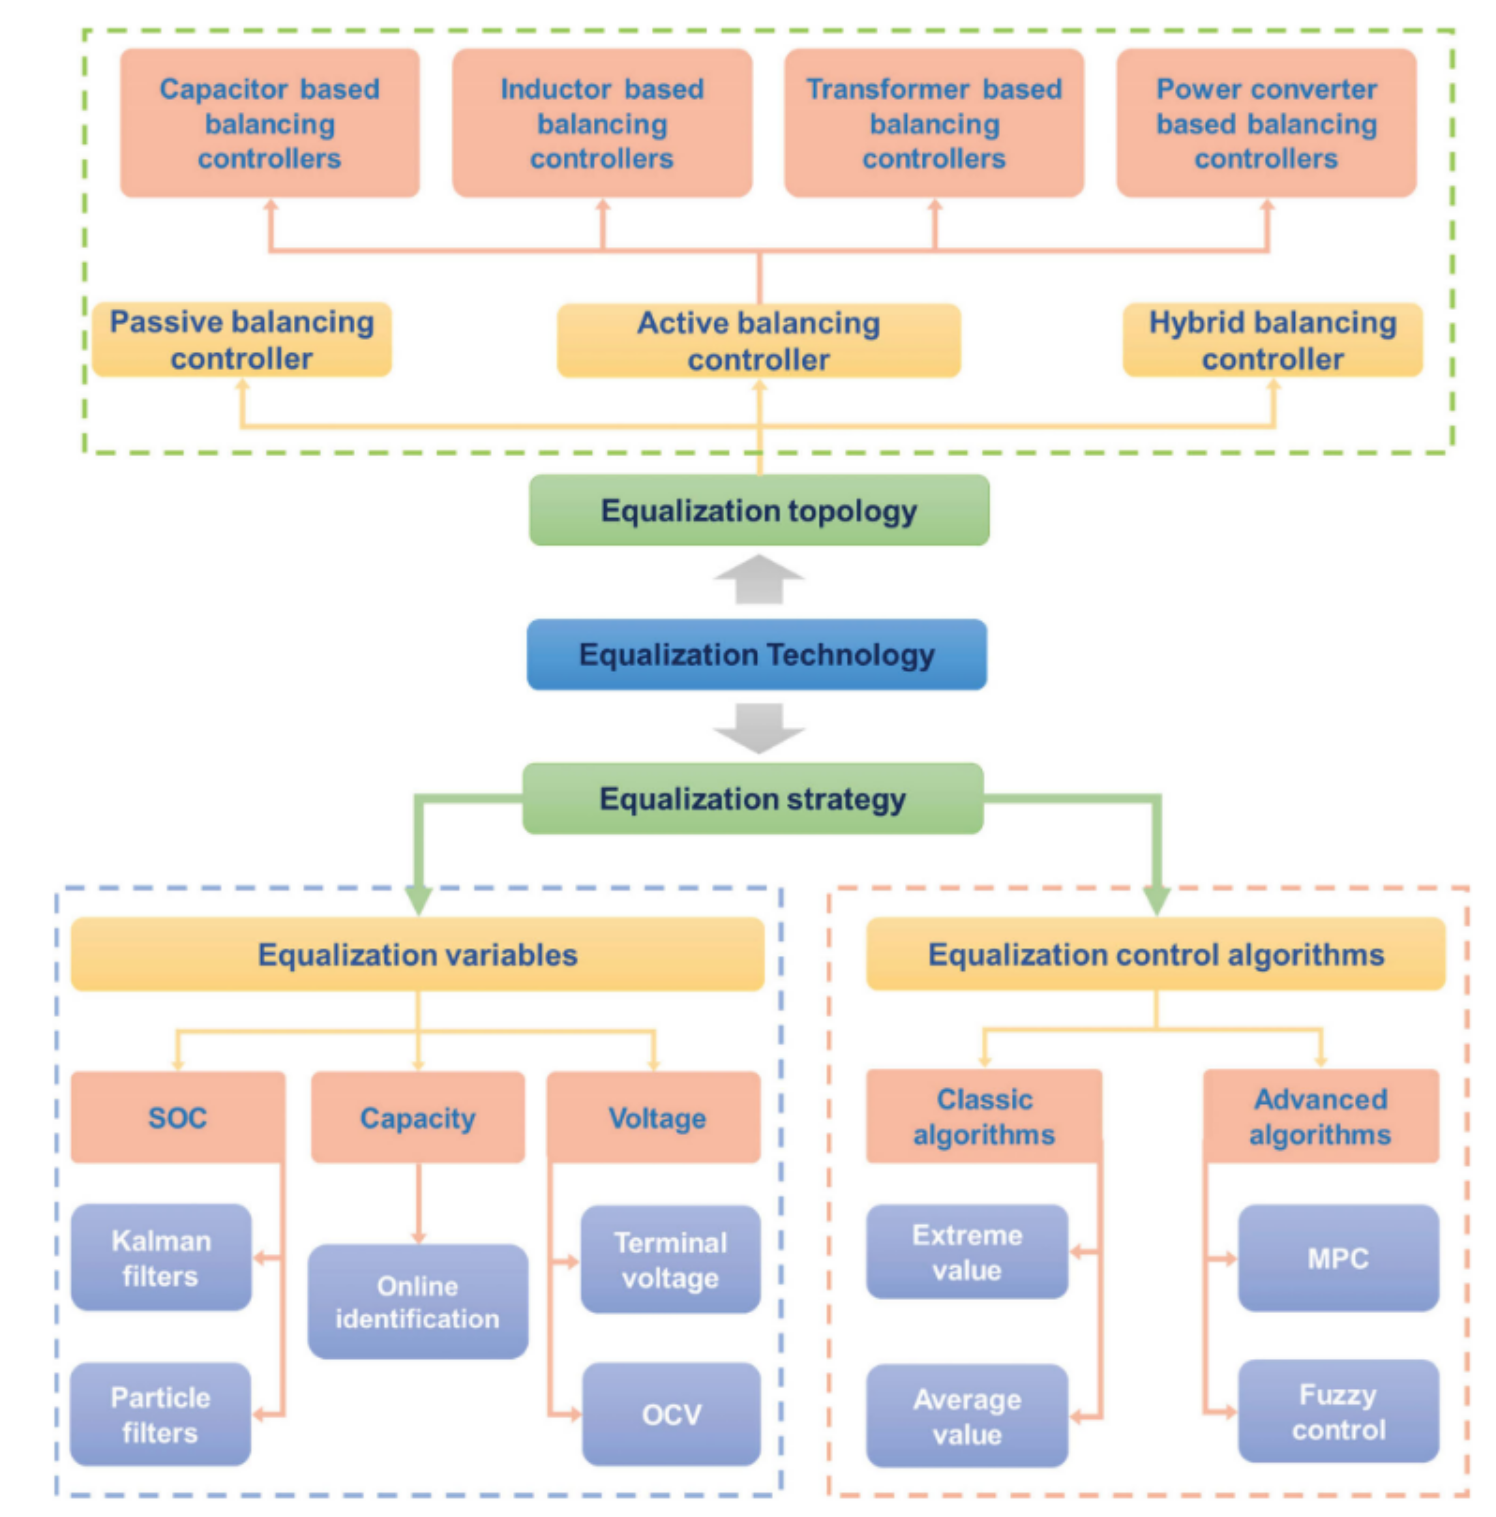
\includegraphics[width=0.75\textwidth]{ems_class.png}
        \caption{Clasificaciones t\'ipicas de los \acrshort{EMS}}
        \label{ems_classes}
    \end{center}
\end{figure}

Como se observa en la Figura \ref{passive_eq_top}, la topolog\'ia de
ecualizaci\'on pasiva generalmente emplea una resistencia en paralelo para
disipar la energ\'ia excesiva. Como se muestra en las Figuras
\ref{energy_transfer} a \ref{hier_bal_top}, las topolog\'ias activas pueden
tranferir energ\'ia entre celdas, m\'odulos y packs con la ayuda de estructuras
que no disipan energ\'ia, tales como inductores y capacitores. Ambas
topolog\'ias son beneficiosas en desacelerar la degradaci\'on de un pack de
bater\'ias extendiendo su vida \'util.

Los \acrshort{EMS} son aplicados en condiciones est\'aticas o semi-est\'aticas 
como por ejemplo, en el proceso de fin de carga, aunque investigaciones 
recientes mostraron aplicaciones de balanceo bajo condiciones din\'amicas del 
proceso de carga y descarga. En \cite{shen_cell_bal} se propone un esquema de 
ecualizaci\'on activa que comienza el trabajo una vez que la bater\'ia est\'a
completamente cargada o descargada para minimizar la transferencia de carga 
durante el proceso de balanceo.

\subsubsection{Control de balanceo pasivo}\label{seq:balanceo_pasivo}

Los controladores de balanceo pasivos (del ingl\'es
\emph{\acrfull{PBC}}) generalmente emplean resistencias \emph{shunt} en paralelo
con las bater\'ias para disipar la energ\'ia excesiva de las celdas con alto
voltaje o alto \acrshort{SOC}.

Como se muestra en la Figura \ref{passive_eq_top}A, el \acrshort{PBC} puede
controlar switches dedicados ($\mathrm{K_1}$, $\mathrm{K_2}$, ...,
$\mathrm{K_n}$), t\'ipicamente semiconductores como MOSFETs, que disipan
energ\'ia de las celdas correspondientes. Por ejemplo, asumiendo que la celda 1
tiene mayor energ\'ia que el resto, entonces el interruptor $\mathrm{K_1}$ se 
cierra para descargar esta celda. El camino de la energ\'ia es indicado por la 
línea a trazos de color azul. Dependiendo de la estrategia de ecualizaci\'on, 
los interruptores pueden funcionar continuamente o de forma intermitente, y la
energ\'ia disipada por la resistencia \emph{shunt} puede ser estimada por la
ley de Joule (\emph{Eq. \ref{joule_law}}).

\begin{equation}
    Q_{disipada} = I^2_{balanceo}R \label{joule_law}
\end{equation}

Donde $\mathrm{Q_{disipada}}$ es la potencia disipada, $\mathrm{I_{balanceo}}$
es la corriente de \emph{bypass} que circula por la resistencia \emph{shunt}, y
R es el valor de la resistencia \emph{shunt}.

La t\'ecnica \acrshort{PBC} es popular en los \acrshort{VVEE} debido a su simple
topolog\'ia y baja complejidad. Sin embargo, posee desventajas tales como la
baja eficiencia de balanceo y largos tiempos de ecualizaci\'on debido a su
limitada potencia de disipaci\'on por los componentes pasivos, limitando su
aplicaci\'on particularmente para bater\'ias de alta capacidad.

En \cite{CAMPESTRINI2016142} se estudia el balanceo pasivo tradicional de celdas 
de litio-ion usando 8 m\'odulos conectados en serie, cada uno compuesto por 14 
celdas conectadas en paralelo (8s14p). Los resultados muestran que los m\'odulos 
con \acrshort{PBC} tienen menos de 1\% de variaci\'on en capacidad despu\'es de 
1200 ciclos. Sin embargo, la celda utilizada en este estudio tiene una capacidad
nominal de 2800mAh que no es suficiente para predecir el efecto de la
ecualizaci\'on de esta t\'ecnica sobre bater\'ias de alta capacidad.

Para incrementar la corriente de balanceo, \cite{XU20192948} propone el 
desarrollo de una topolog\'ia de balanceo especial, en donde la resistencia 
shunt es reemplazada por un MOSFET, como se puede observar en la Figura
\ref{passive_eq_top}B. Por ejemplo, asumiendo que la celda 2 tiene mayor
energ\'ia que el resto, entonces el MOSFET $\mathrm{S_2}$ funciona como una
resistencia \emph{shunt} mientras que el resto permanece apagado. 

En \cite{amin_et_al_bal} se propone una topolog\'ia de balanceo pasiva que 
combina una resistencia shunt con MOSFETs. El \acrshort{PBC} fue implementado 
en un pack de 15 celdas $\mathrm{LiFePO_4}$ con una capacidad de 200Ah. Sin 
embargo, el proceso de balanceo toma mucho tiempo bajo condiciones de 
operaci\'on.

En \cite{SCHMID201749} se propone una topolog\'ia de ecualizaci\'on denominada 
\emph{balanceo electroqu\'imico} para balancear celdas sin dispositivos 
electr\'onicos adicionales que consite en conectar cada celda en serie con una 
celda de n'iquel-metal o n'iquel-zinc en paralelo. Las celdas de litio-ion pueden 
alcanzar la ecualizaci\'on con el proceso electroqu\'imico de las celdas de 
n'iquel. Los resultados verifican que este m\'etodo es posible de implementar, 
sin embargo hay una limitaci\'on de costos, volumen y complejidad muy alta.

\begin{figure}[h!]
    \begin{center}
        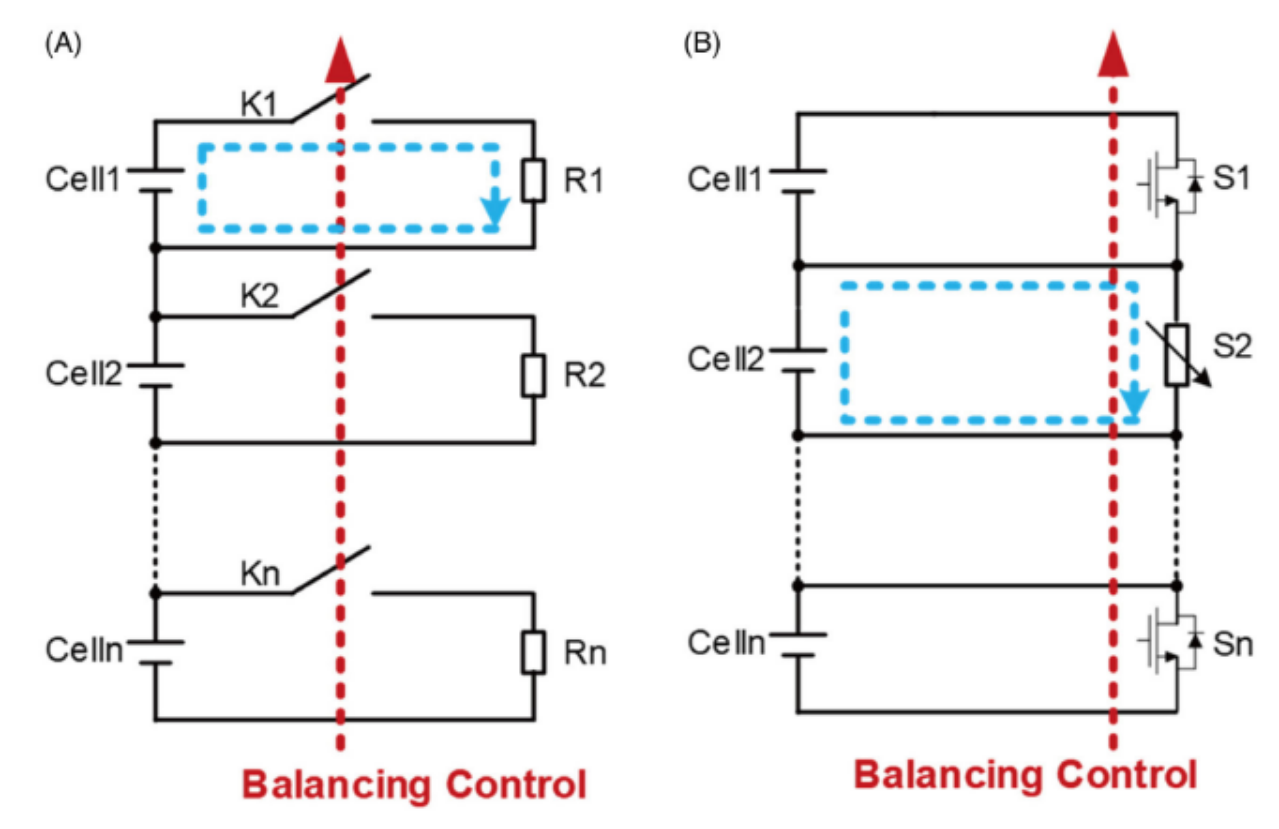
\includegraphics[width=0.75\textwidth]{passive_eq_top.png}
        \caption{Topolog\'ia de un circuito balanceador pasivo. (A) Resistencia
        tradicional con baja corriente de balanceo. (B) Topolog\'ia basada en
        MOSFET que utiliza $\mathrm{R_{DS_{on}}}$ soportando altas corrientes.}
        \label{passive_eq_top}
    \end{center}
\end{figure}

\subsubsection{Controlador de Balanceo Activo}

Los controladores de balanceo activo (\acrshort{ABC}, del ingl\'es \acrlong{ABC})
tienen topolog\'ias que, en vez de disipar energ\'ia, la transfieren entre
distintas celdas y m\'odulos/packs usando varios dispositivos que act\'uan como
\emph{buffers} de energ\'ia, incluyendo capacitores, transformadores, inductores
y convertidores de potencia.

Las principales ventajas de los \acrshort{ABC}s consiste en alta eficiencia,
alta velocidad y alta precisi\'on. Sin embargo, comparado con los 
\acrshort{PBC}s, los \acrshort{ABC}s tienen que enfrentar ciertas dificultades, 
como por ejemplo estructuras complejas, grandes tamaños y sistemas costosos de 
implementar.

\subsubsubsection{Camino de transferencia de energ\'ia}

Una de las ventajas superiores de los \acrshort{ABC}s es que la energ\'ia se
puede transferir entre distintos niveles para alcanzar un balanceo del sistema,
que reduce el consumo de energ\'ia cuando se busca lograr la ecualizaci\'on del
pack de bater\'ias. Considerando el camino de esta transferencia de energ\'ia,
los \acrshort{ABC}s pueden clasificarse en balanceo entre celda-a-celda
(\acrshort{C2C}, del ingl\'es \emph{\acrlong{C2C}}), balanceo entre
celda-a-m\'odulo (\acrshort{C2M}, del ingl\'es \emph{\acrlong{C2M}}), balanceo
entre m\'odulo-a-celda (\acrshort{M2C}, del ingl\'es \emph{\acrlong{M2C}}). La
flexibilidad en la transferencia de energ\'ia se puede observar en la Figura
\ref{energy_transfer}.

Como se observa en la Figura \ref{energy_transfer}A, la ecualizaci\'on
\acrshort{C2C} denota que la energ\'ia puede ser transferida entre las celdas de
un mismo m\'odulo/pack, que es el modo fundamental de los \acrshort{ABC}s. En
\cite{phung_bal} se presenta una arquitectura \acrshort{C2C} optimizada que se 
basa en la topolog\'ia tradicional de balanceo contiguo, que es m\'as compacto y 
f\'acil de implementar. Para n celdas conectadas en series, la arquitectura 
\acrshort{C2C} generalmente necesita n-1 componentes de transferencia de 
energ\'ia. Por lo tanto, a medida que aumenta el n\'umero de celdas conectads en
serie, el circuito se hace m\'as complicado de implementar.

Como se muestra en la Figura \ref{energy_transfer}B, la ecualizaci\'on
\acrshort{C2M} puede transferir energ\'ia entre el m\'odulo  y la celda interna
de forma bidireccional, que tiene la ventaja de desaparear la inconsistencia
entre los m\'odulos de las bater\'ias. Los autores en \cite{lu_et_al_bal} 
proponen un controlador aislado bidireccional tipo \acrshort{C2M} con una 
conmutaci\'on suave a cero voltaje. Cuando funciona en modo \emph{boost}, el 
convertidor puede transferir energ\'ia de la bater\'ia al m\'odulo, mientras que 
cuando funciona en modo \emph{buck} la transferencia de energ\'ia se realiza 
desde el m\'odulo a la celda descargada. \'Esta metodolog\'ia demuestra 
resultados experimentales con buen rendimiento tanto en velocidad como 
eficiencia.

La Figura \ref{energy_transfer}C muestra una arquitectura \acrshort{M2M}
donde la transferencia de energ\'ia se realiza entre m\'odulos. Comparado con
las arquitecturas \acrshort{C2C} y \acrshort{C2M}, la arquitectura 
\acrshort{M2M} generalmente tiene un tamaño considerablemente grande teniendo en 
cuenta la aislaci\'on de corriente y una estrategia compleja para evitar el 
desbalanceo, haciendo que esta implementaci\'on sea m\'as dificultosa que el 
resto. En \cite{ji_et_al_bal_mod} se propone un esquema de ecualizaci\'on usando 
m\'ultiples transformadores que con permiten que la energ\'ia pueda ser 
transferida entre m\'odulos de distintos voltajes, alcanzado una corriente de 
balanceo de hasta 3A mientras que la inconsistencia entre voltajes es de 24mV.

Otros m\'etodos no ilustrados en la Figura \ref{energy_transfer} tambi\'en
fueron estudiados. Por ejemplo, en \cite{li_et_al_bal} se propone una 
topolog\'ia de ecualizaci\'on m\'odulo-a-celda-a-m\'odulo. Con la ayuda de 
conmutaci\'on suave a cero voltaje y un circuito bidireccional resonante, la 
velocidad y eficiencia del m\'etodo puede ser mejorado de forma considerable. 
Los resultados experimentales muestran que la topolog\'ia puede obtener una 
eficacia del 93\% en modo \acrshort{C2M} y 72.5\% en modo \acrshort{M2C}.

\begin{figure}[h!]
    \begin{center}
        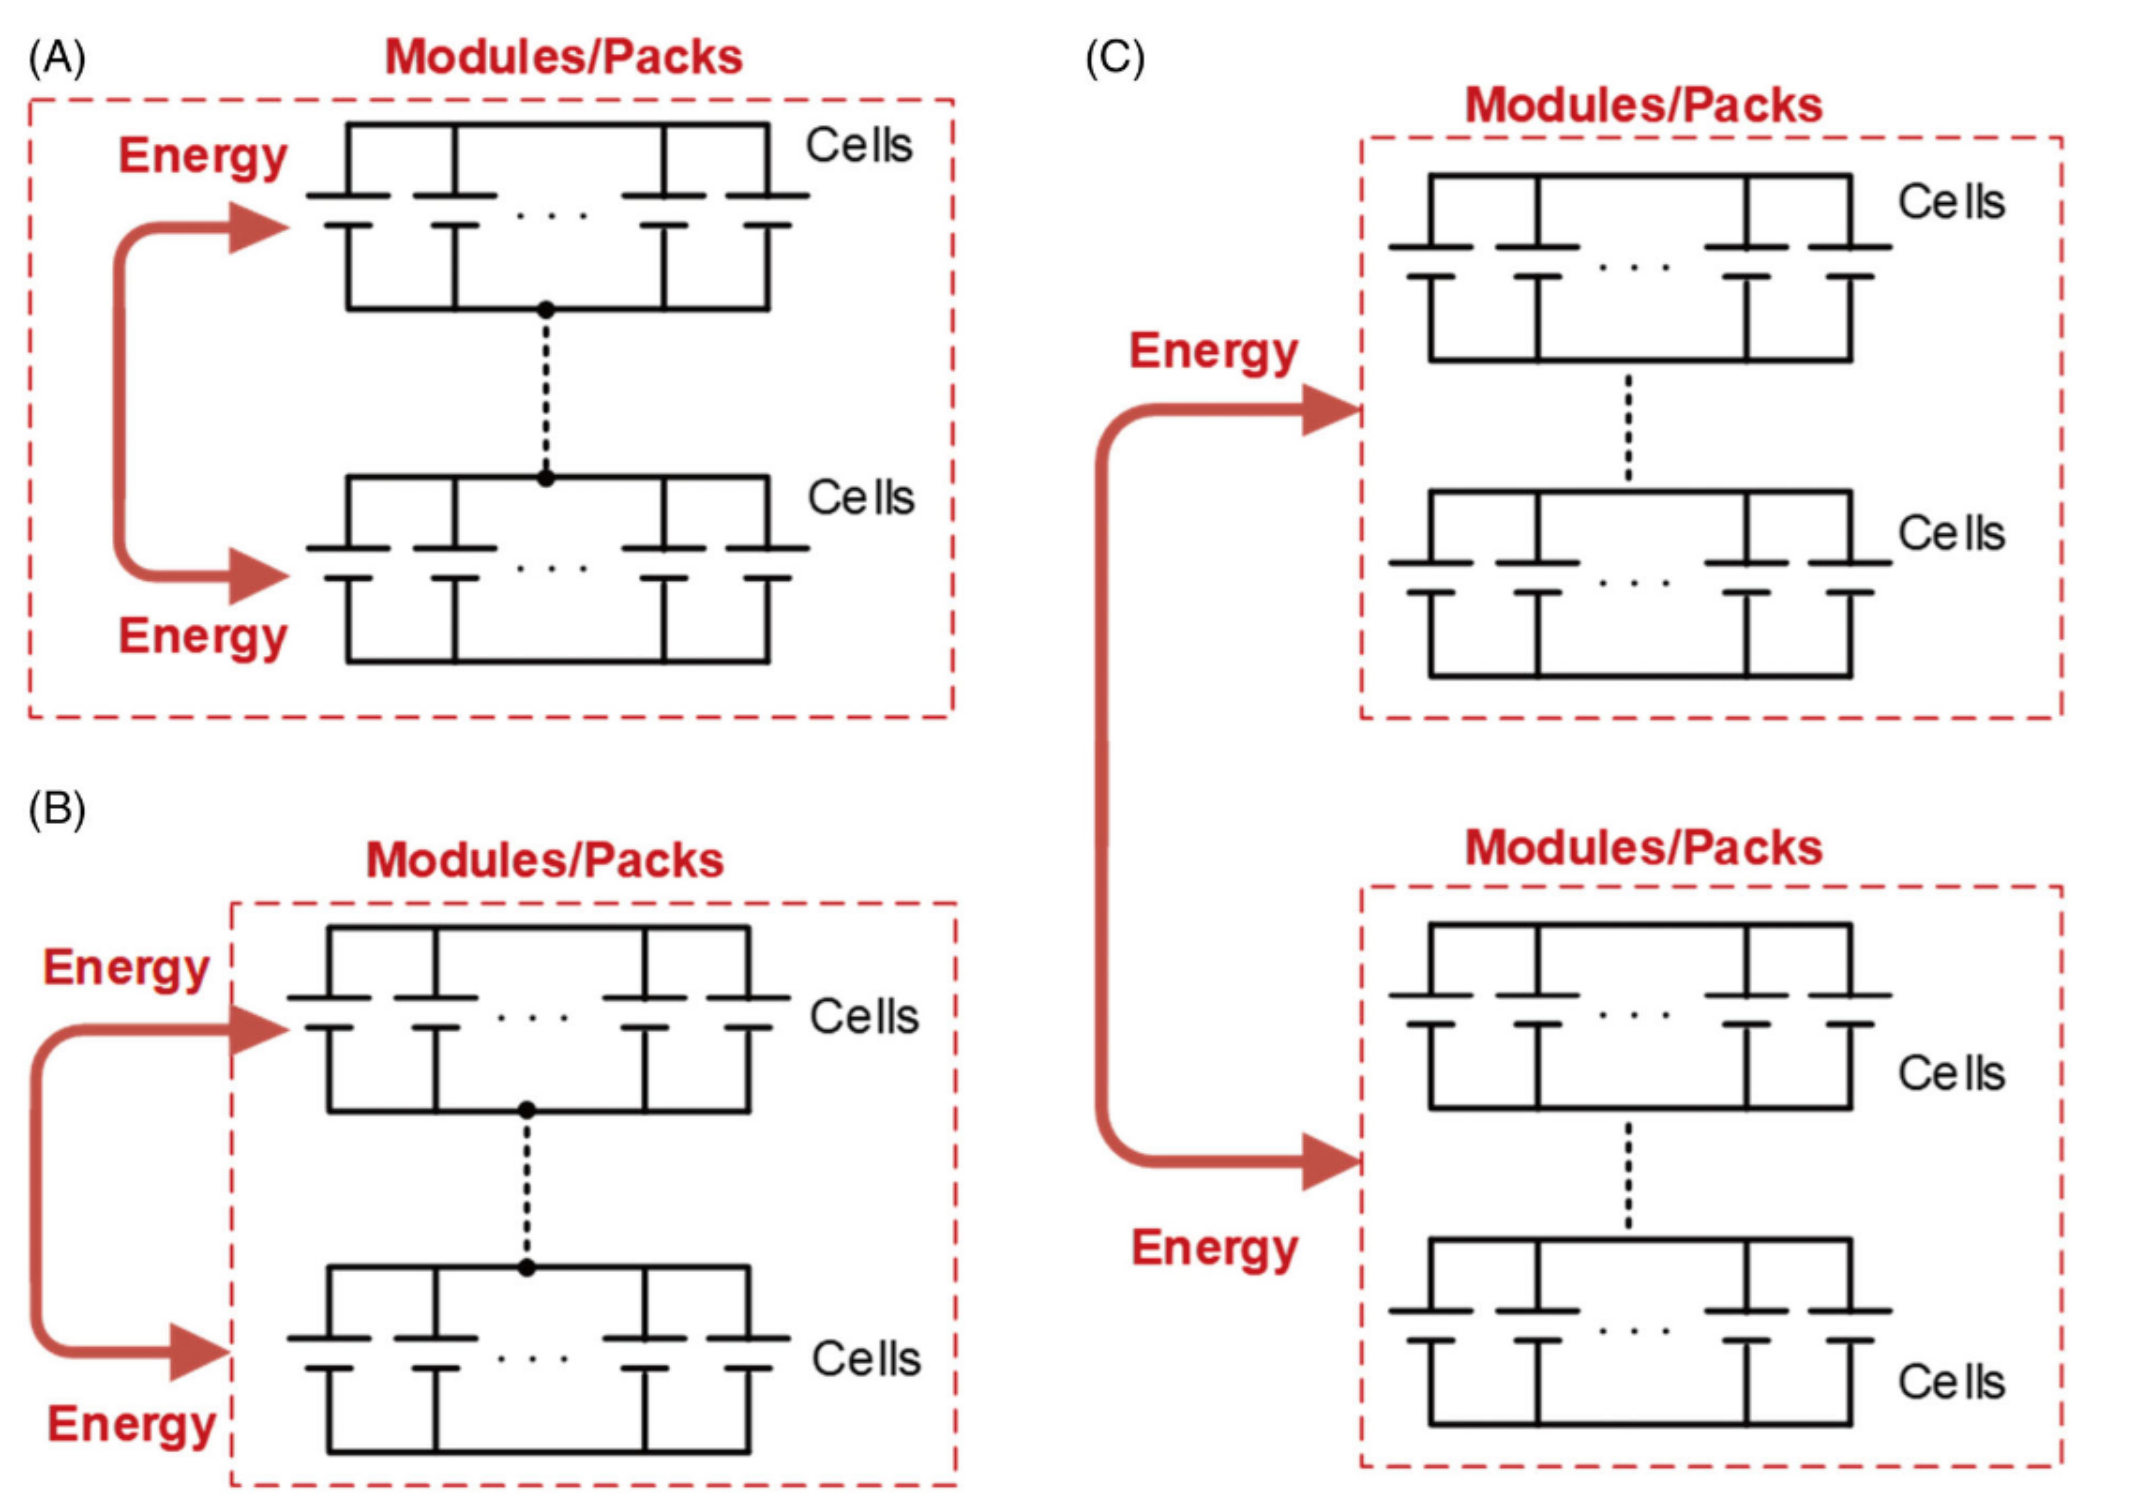
\includegraphics[width=0.8\textwidth]{energy_transfer.png}
        \caption{Diferentes caminos de transferencia de energ\'ia. (A)
        Celda-A-Celdas (\acrshort{C2C}). (B) Celda-A-M\'odulo (\acrshort{C2M}).
        (C) M\'odulo-A-M\'odulo (\acrshort{M2M})} 
        \label{energy_transfer}
    \end{center}
\end{figure}

\subsubsubsection{Controlador de balanceo basado en capacitores}

Los controladores de balanceo basados en capacitores (\acrshort{CBBC}, del
ingl\'es \emph{\acrlong{CBBC}}) pueden transportar energ\'ia entre celdas o
entre celdas, m\'odulos y sistemas.

Como se muestra en la Figura \ref{cbbc_top}, los \acrshort{CBBC}s pueden ser 
clasificados en una topolog\'ia de un solo capacitor, capacitor alternado y una 
topolog\'ia de capacitores multi-capa. Los \acrshort{CBBC} solo pueden 
transferir energ\'ia entre bater\'ias que poseen un voltaje de diferencia 
significativo.

Una t\'ipica topolog\'ia de un solo capacitor se puede observar en la Figura
\ref{cbbc_top}A, que adem\'as de poseer un solo capacitor (C), est\'a compuesto
de varios interruptores unipolares (\acrshort{SPST}, del ingl\'es 
\emph{\acrlong{SPST}}) y bipolares (\acrshort{SPDT}, del ing\'es 
\emph{\acrlong{SPDT}}). 

La topolog\'ia \acrshort{CBBC} con un solo capacitor, con una estrategia de
control muy simple y baja p\'erdida de energ\'ia, tiene la desventaja de que el
tiempo de balanceo es extenso. Durante la operaci\'on, el ecualizador detecta
las celdas con mayores y menores voltajes, y despu\'es realiza la transferencia
de energ\'ia entre las celdas seleccionados con el control de los
\acrshort{SPST}. El proceso de ecualizaci\'on comienza con la carga del
capacitor por la bater\'ia de alto voltaje y contin\'ua con la descarga del
capacitor en la celda de bajo voltaje. Por ejemplo, asumiendo que la celda 1 y
la celda 2 son las celdas con el mayor y el menor voltaje respectivamente,
inicialmente, los \acrshort{SPST} $\mathrm{K_1}$ y $\mathrm{K_2}$ son conectados
con el lado de bajo voltaje y los \acrshort{SPDT} $\mathrm{S_1}$ y 
$\mathrm{S_2}$ son conectados al lado de alto voltaje, provocando la
transferencia de la energ\'ia desde la celda 1 al capacitor C como se muestra en
la línea azul. Una vez cargado el capacitor, $\mathrm{K_1}$ es desconectado,
mientras que $\mathrm{K_2}$ y $\mathrm{K_3}$ se cierran, por el otro lado
$\mathrm{S_1}$ y $\mathrm{S_2}$ son conectados al lado bajo y la energ\'ia
ser\'a transferida desde el buffer hasta la celda 2 como se muestra en la línea
verde.

Una topolog\'ia t\'ipica de un capacitor alternado se muestra en la Figura
\ref{cbbc_top}B, que consiste de varios capacitores y \acrshort{SPDT}s para
transmitir energ\'ia entre bater\'ias contiguas con el control de los
interruptores. Los \acrshort{CBBC}s con esta toplog\'ia tienen ventajas 
similares a la estructura de un solo capacitor, como por ejemplo, una estructura 
simple y de bajo costo, pero requiere de una estrategia de control finamente 
ajustada, especialmente cuando hay una pequeña diferencia de voltaje entre las 
celdas adyacentes. Las líneas azul y verde muestran como es el camino de 
transferencia de la energ\'ia.

La Figura \ref{cbbc_top}C muestra una topolog\'ia de capacitores de dos capas
que transfiere energ\'ia entre celdas adyacentes a trav\'es de la primer capa y
transfiere energ\'ia entre las bater\'ias que no est\'an conectadas de forma
directa a trav\'es de la segunda capa, reduciendo significativamente el tiempo
de ecualizaci\'on. La línea azul muestra la transferencia de energ\'ia entre la
celda 1 y la celda 2 a un capacitor de la segunda capa ($\mathrm{C_{21}}$), y la
energ\'ia puede ser transferida desde $\mathrm{C_{21}}$ a la celda 2 y 3 para
lograr la transmisi\'on de la celda 1 a la 3 como se muestra en la línea verde. 

Una topolog\'ia t\'ipica multicapa se puede observar en la Figura
\ref{cbbc_top}D. Adem\'as de la transferencia entre celdas del mismo m\'odulo,
esta topolog\'ia nos permite transmitir energ\'ia entre m\'odulos. 

Por \'ultimo, a pesar de las t\'ipicas estructuras todav\'ia se encuentran
en desarrollo e investigaci\'on nuevas tecnolog\'ias basadas en capacitores,
como por ejemplo, en \cite{shang_et_al_bal_cap} se propone un ecualizador de 
capacitores basados en una estructura de tipo malla (del ingl\'es \emph{mesh}) 
que mejora de manera significativa la eficiencia y velocidad del balanceo. 
Su estructura se puede observar en la Figura \ref{cbbc_mesh_top}

\begin{figure}[h!]
    \begin{center}
        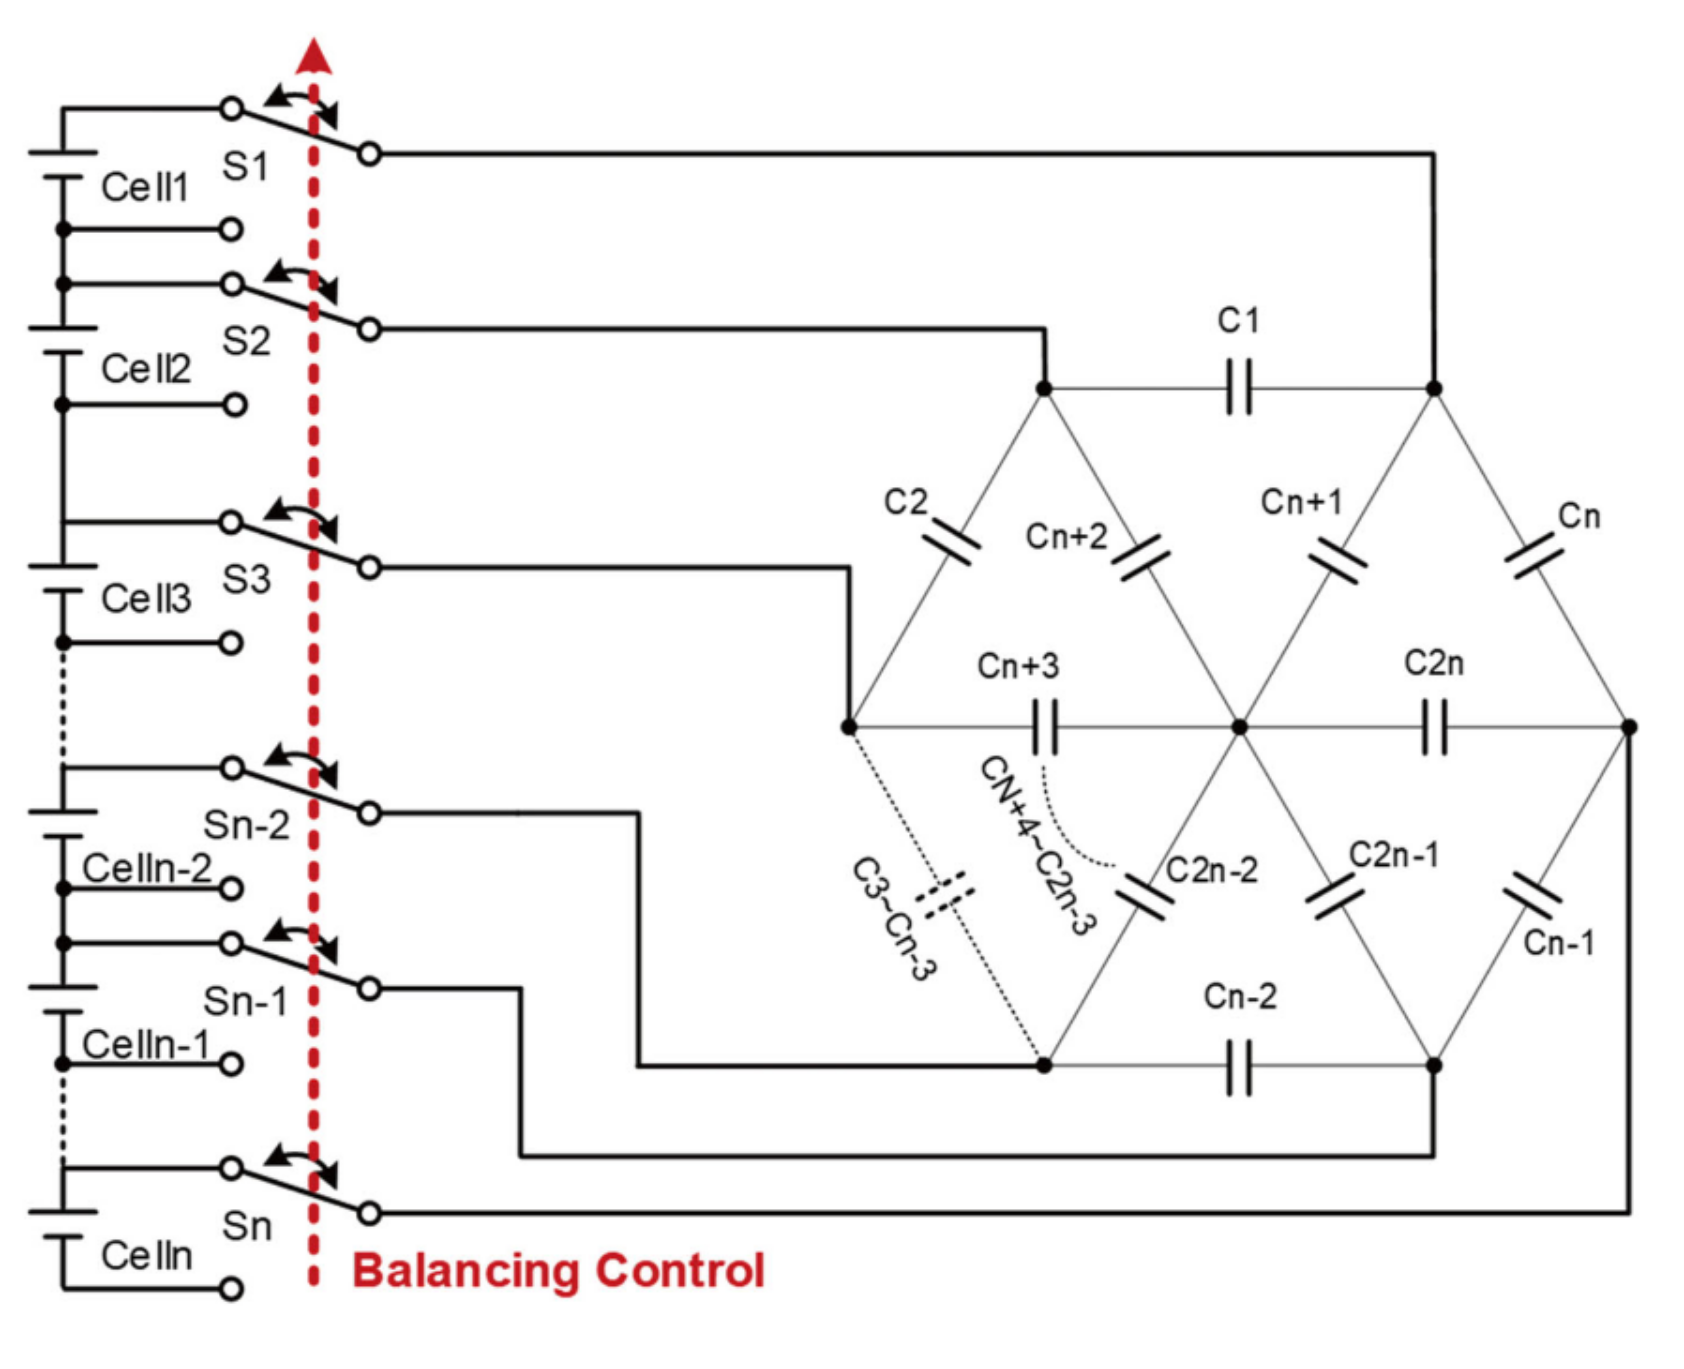
\includegraphics[width=0.7\textwidth]{cbbc_mesh_top.png}
        \caption{Balanceador de celdas basado en capacitores con una topolog\'ia
        de tipo red.}
        \label{cbbc_mesh_top}
    \end{center}
\end{figure}

\begin{figure}[h!]
    \begin{center}
        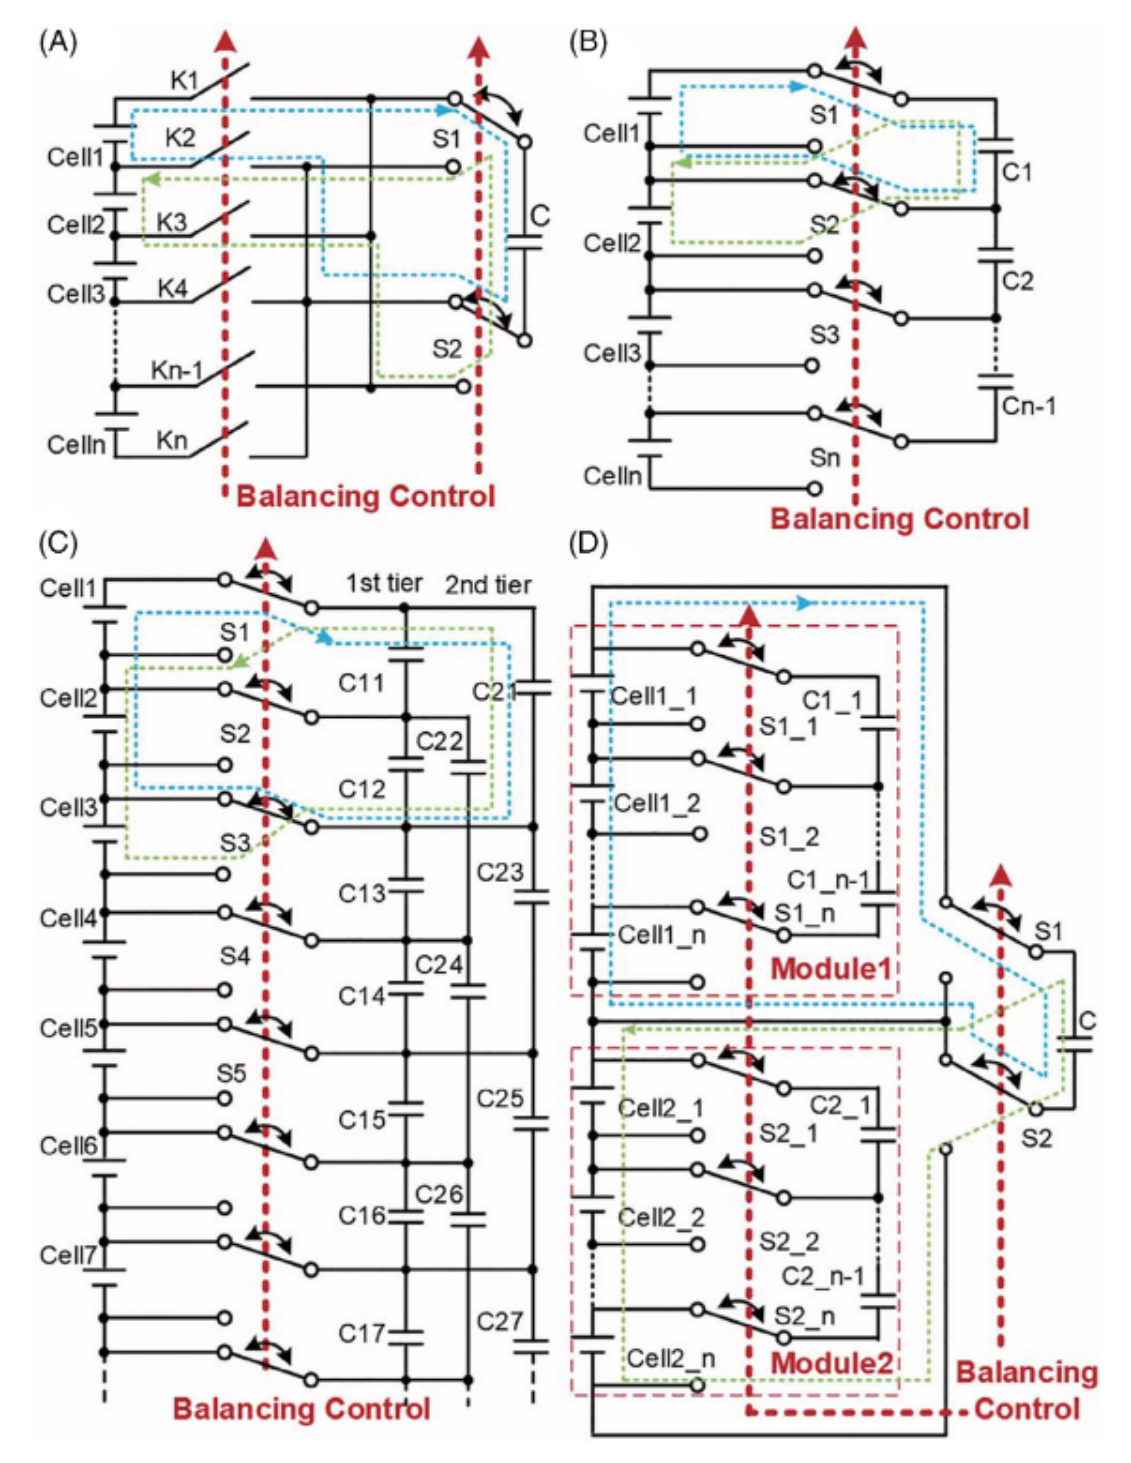
\includegraphics[width=0.8\textwidth]{cbbc_top.png}
        \caption{Topolog\'ias de balanceo basada en capacitores. (A) Topolog\'ia
        de capacitor simple (\acrshort{C2C}). (B). Topolog\'ia de capacitores
        alternantes (\acrshort{C2C}). (C) Topolog\'ia basada en dos capas de
        capacitores (\acrshort{C2C}). (D) Topolog\'ia de capacitores multi-capa
        (\acrshort{C2C})}
        \label{cbbc_top}
    \end{center}
\end{figure}

%\newpage

\subsubsubsection{Controlador de balanceo basado en inductores}

Los controladores de balanceo basado en inductores (\acrshort{IBBC}, del
ingl\'es \acrlong{IBBC}) pueden transferir energ\'ia entre celdas y m\'odulos a
trav\'es de inductores externos. Comparado con los \acrshort{CBBC}s, los
\acrshort{IBBC}s t\'ipicamente est\'an relacionados con velocidades de balanceo
m\'as r\'apidas debido a una corriente de ecualizaci\'on m\'as alta, sin embargo
\acrshort{IBBC}s son generalmente m\'as costosos y menos eficientes.

Los \acrshort{IBBC}s pueden ser clasificado entre distintas topolog\'ias, como por
ejemplo, una topolog\'ia de un inductor simple o inductores alternativos, como
se observa en la Figura \ref{ibbc_top}.

\begin{figure}[h!]
    \begin{center}
        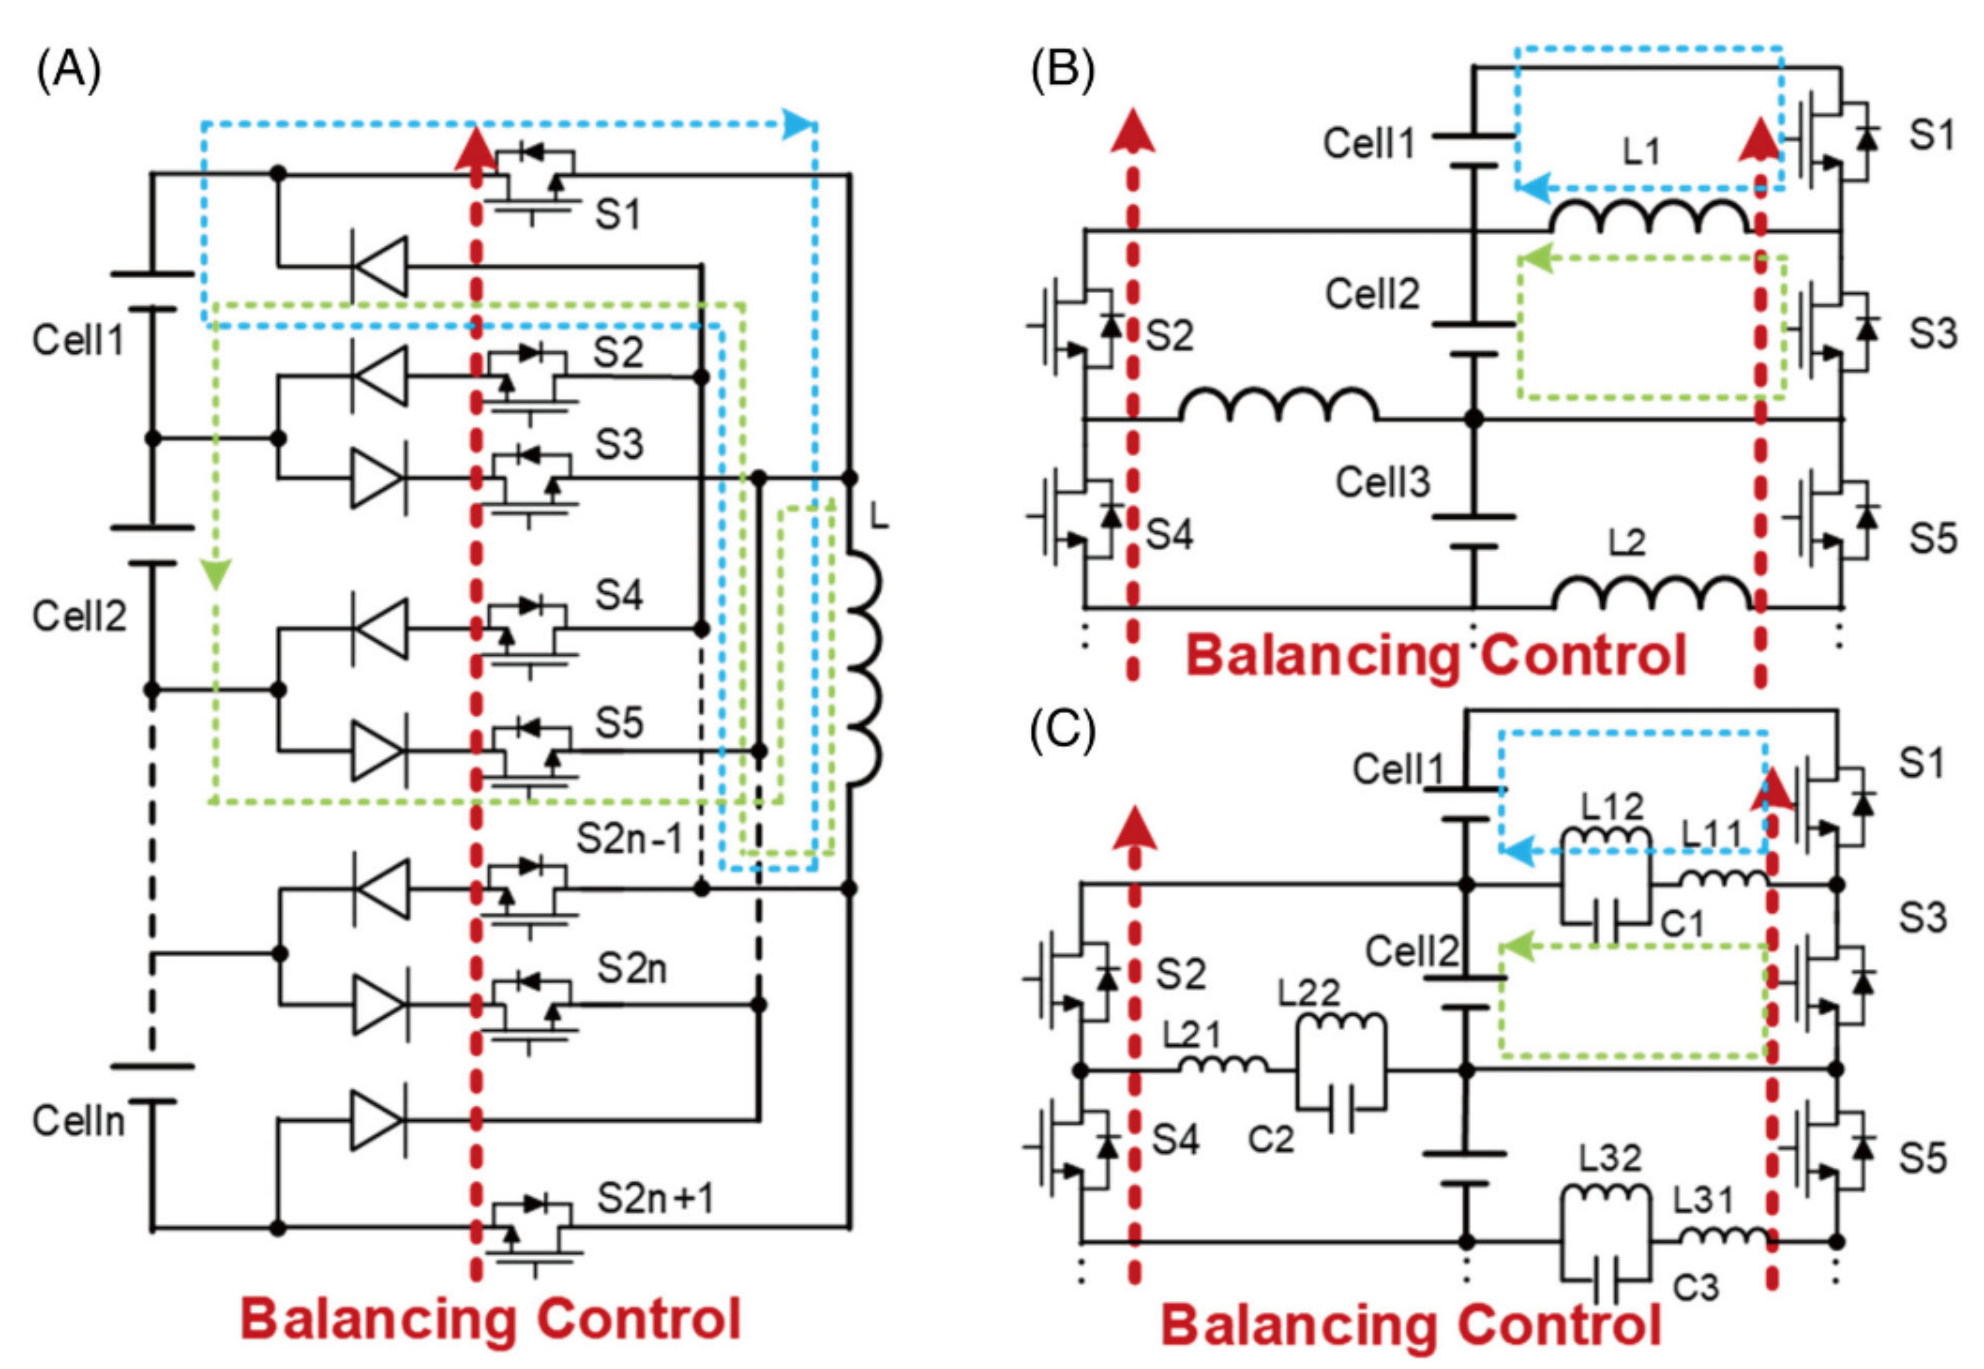
\includegraphics[width=0.8\textwidth]{ibbc_top.png}
        \caption{topolog\'ias de balanceo basadas en inductores. (A) Topolog\'ia
        de inductor simple (\acrshort{C2C}). (B) Topolog\'ia de m\'ultiples
        inductores (\acrshort{C2C}). (C) Topolog\'ia de inductores resonantes
        (\acrshort{C2C})}
        \label{ibbc_top}
    \end{center}
\end{figure}

Una topolog\'ia t\'ipica de inductor simple se puede observar en la
Figura\ref{ibbc_top}A, que incluye un solo inductor y varios MOSFETs que permite
transferir la energ\'ia entre celdas seleccionadas controlando los MOSFETs con
señales \acrshort{PWM} (del ingl\'es \emph{\acrlong{PWM}}). Por ejemplo, 
asumiendo que la celda 1 y 2 son las celdas con mayor y menor voltaje 
respectivamente. Los MOSFETs S1 y S2 son inicialmente encendidos, permitiendo 
que la energ\'ia se transfiera de la celda 1 a la inductancia L, como muestra la 
línea azul. La energ\'ia transferida se puede calcular con la Ecuaci\'on 
\ref{energy_trans_ind}:

\begin{equation}
    \dot{Q} = UI = IL\frac{dI}{dt} \label{energy_trans_ind}
\end{equation}

donde L es el valor de la inductancia, U e I son la tensi\'on de los terminales
de la bater\'ia y la corriente que circula por el inductor respectivamente.
Entonces cuando el interruptor S1 se apaga y se enciende S5, la energ\'ia se
transfiere desde la inductancia a la celda 2 como muestra la línea verde.
Las señales \acrshort{PWM} son utilizadas como señales de control que comandan 
los MOSFETs para transferir energ\'ia entre las celdas.

Una configuraci\'on t\'ipica de m\'ultiples inductores se puede observar en la
Figura \ref{ibbc_top}B, que consiste de varios inductores y MOSFETs. La
energ\'ia transferida entre celdas es, nuevamente, controlada por los MOSFETs. 
Las líneas azules y verdes muestran los caminos de transferencia de 
energ\'ia para la descarga de la celda 1 y la carga de la celda 2. La velocidad 
de ecualizaci\'on para tales topolog\'ias se encuentra afectada por la escala 
del pack, y la velocidad es generalmente baja porque la transferencia de 
energ\'ia solo se puede realizar entre celdas adyacentes.

En la Figura \ref{ibbc_top}C se muestra un circuito de inductor resonante. Este
circuito es utilizado como reemplazo del inductor simple, debido a que puede
reducir la interferencia electromagn\'etica (\acrshort{EMI}, del ingl\'es
\emph{\acrlong{EMI}}) e incrementar las p\'erdidas provocadas por la
conmutaci\'on durante el proceso de ecualizaci\'on. Las líneas azul y verde
muestran el intercambio de energ\'ia para la descarga de la celda 1 y la carga
de la celda 2 respectivamente.

%Note: (FDC) No logro ver como podríamos pasar energía con una inductancia desde
%una delda de menor voltaje a una de mayor

%Una caracter\'istica particular de los circuitos \acrshort{IBBC}s es que la
%transferencia de energ\'ia se puede hacer desde una celda con menor voltaje a
%una celda de mayor voltaje. Por lo tanto, la estrategia de balanceo debe ser
%considerada cuidadosamente para evitar un error de balanceo.

\subsubsubsection{Controlador de balanceo basado en transformadores}

Los controladores de balanceo basados en transformadores (\acrshort{TBBC}, del
ingl\'es \emph{\acrlong{TBBC}}) pueden transferir energ\'ia entre distintas celdas y
m\'odulos a trav\'es de transformadores externos. Como se muestra en la Figura
\ref{tbbc_top}, los \acrshort{TBBC} se pueden dividr en transformadores de
devanado simple o transformadores de m\'ultiples devanados.

\begin{figure}[h!]
    \begin{center}
        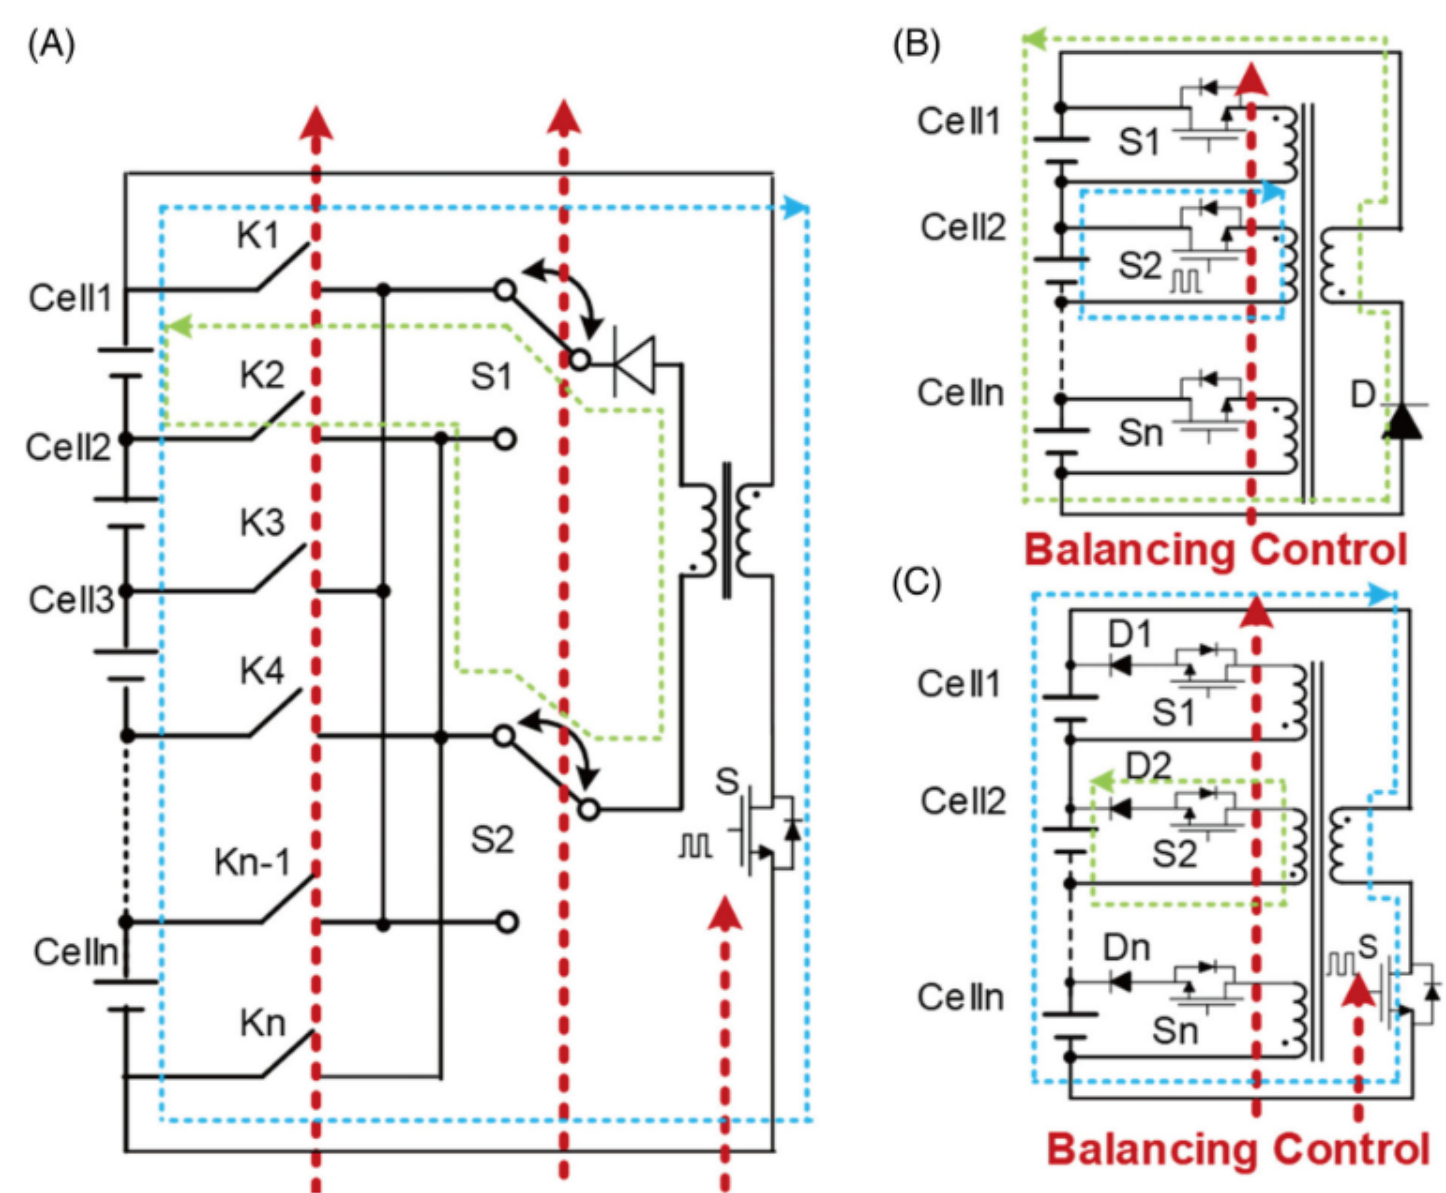
\includegraphics[width=0.75\textwidth]{tbbc_top.png}
        \caption{Topolog\'ias de balanceo basados en transformadores. (A)
        topolog\'ia basada en un transformador de devanado simple
        (\acrshort{M2C}). (B) Topolog\'ia de tranformadores de devanados
        m\'ultiples (\acrshort{C2M}). (C) Topolog\'ia de transformadores de
        devanados m\'ultiples (\acrshort{M2C})}
        \label{tbbc_top}
    \end{center}
\end{figure}

En la Figura \ref{tbbc_top}A se puede observar una topolog\'ia \acrshort{TBBC}
basada en un transformador de devanado simple, que puede transferir energ\'ia de
forma \acrshort{M2C} controlando los interruptores del circuito. Por ejemplo,
asumiendo que la celda 1 es la celda con la mejor energ\'ia. Inicialmente, el
MOSFET S se cierra y comienza a circular corriente desde el m\'odulo hacia el
transformador. La línea azul muestra el camino de esta transferencia de
energ\'ia. Una vez que el MOSFET S se apaga, los interruptores S1 y S2 son
conectados a la parte alta y baja de la celda 1 respectivamente, y la energ\'ia
almacenada en el transformador es transferida a la misma. La línea verde muestra
como se transfiere la energ\'ia desde el transformador a la celda 1. Una primer
desventaja para este tipo de topolog\'ia, que se puede observar a simple vista,
es que se necesitan transformadores de alto voltaje lo que implica un costo alto
y un gran tamaño para ser implementado, sin contar el peso, característica
fundamental a tener en cuenta en los vehículos eléctricos.

Una topolog\'ia de m\'ultiples devanados para una transferencia de energ\'ia
\acrshort{C2M} se puede observar en la Figura \ref{tbbc_top}B. Por ejemplo,
asumiendo que la celda 2 es la celda con mayor energ\'ia, el MOSFET S2 se
enciende y la corriente comienza a circular hacia el transformador en el sentido
directo. Una vez que el MOSFET S2 se apaga, la energ\'ia almacenada en el
transformador ser\'a transferida al m\'odulo. Las líneas azul y verde muestran
los caminos de esta transferencia de energ\'ia.

Por el otro lado, en la Figura \ref{tbbc_top}C se muestra una topolog\'ia basada
en transformadores de m\'ultiples devanados para una transferencia tipo
\acrshort{M2C}. Por ejemplo, asumiendo que la celda 2 es la bater\'ia con menor 
energ\'ia en el pack. Inicialmente, el MOSFET S se enciende y la corriente 
comienza a circular hacia el transformador. Una vez que el MOSFET S se apaga, el
MOSFET S2 se enciende y la energ\'ia almacenada es transferida a la celda 2. Las
señales de \acrshort{PWM} son utilizadas para regular la transferencia de
energ\'ia entre las celdas.

La velocidad de ecualizaci\'on de los \acrshort{TBBC}s son generalmente
r\'apidas, pero los voltajes en el devanado secundario son inconsistentes debido
a p\'erdidas de inductancia en el devanado de los transformadores. Otro gran
problema de estas topolog\'ias es que la fabricaci\'on de devanados sim\'etricos
para aplicaciones de alta potencia son costosos.

\subsubsubsection{Balanceadores basados en convertidores de potencia}

Los convertidores DC/DC, o convertidores de potencia, pueden convertir una fuente
DC de un voltaje a otro distinto. Los controladores de balanceo basados en
convertidores de potencia (\acrshort{PBBC}, del ing\'es \acrlong{PBBC}) tienen
la ventaja de ser altamente eficientes y precisos para la transformaci\'on de
energ\'ia de forma bidireccional. Los \acrshort{PBBC}s pueden transferir la
energ\'ia entre distintas celdas y m\'odulos. Los convertidores de potencia
aplicados en estas topolog\'ias pueden funcionar en modo reductor (del ingl\'es
\emph{buck}), elevador (del ingl\'es \emph{boost}), elevador-reductor, Cuk y
otros tipos. Ya que los convertidores de potencia DC/DC usan inductores o
transformadores como componentes de almacenamiento de energ\'ia, los
\acrshort{PBBC}s tienen algunas similitudes con los \acrshort{IBBC}s e
\acrshort{TBBC}s. Los \acrshort{PBBC}s pueden alcanzar un control muy preciso en 
el proceso de ecualizaci\'on pero con la contraparte de ser costosos y complejos 
de implementar.

El convertidor de potencia reductor disminuye el voltaje de entrada con al menos
dos semiconductores y un inductor. Una topolog\'ia de ecualizaci\'on basada en
un convertidor reductor se puede observar en la Figura \ref{pbbc_top}A. Durante
el proceso de carga, cada circuito reductor puede servir como un circuito de
carga y controlar la corriente de este proceso para cada celda de forma 
independiente. Asumiendo que el circuito reductor funciona en modo de 
conducci\'on continua, el voltaje de cada celda conectada en serie se puede 
expresar en la Ecuaci\'on \ref{pbbc_reduc_voltaje},

\begin{equation}
    V_{mi} = V_{ci} \times D_i \label{pbbc_reduc_voltaje}
\end{equation}

donde $\mathrm{V_{mi}}$ es el voltaje promedio en la i-\'esima celda,
$\mathrm{V_{ci}}$ es el voltaje promedio del capacitor correspondiente, y
$\mathrm{D_i}$ es el ciclo de trabajo de la señal de \acrshort{PWM}. Debido a
que cada m\'odulo trabaja de forma independiente, es posible alcanzar una
ecualizaci\'on del pack en corto tiempo.

Los convertidores de potencia elevadores aumentan la tensi\'on de entrada con
al menos dos semiconductores y un elemento de almacenamiento de energ\'ia. El
esquem\'atico de un circuito de balanceo basado en convertidores elevadores se
puede observar en la Figura \ref{pbbc_top}B. La corriente promedio de todos los
circuitos elevadores son iguales, pero cada corriente individual difiere
dependiendo del voltaje del m\'odulo y el ciclo de trabajo de la señal de
\acrshort{PWM} para alcanzar la ecualizaci\'on.

Los convertidores reductores-elevadores pueden implementar funciones de ambas
topolog\'ias, y el voltaje de salida puede ser mayor o menor al de entrada. Una
topolog\'ia t\'ipica que implementa estos convertidores se puede observar en
\ref{pbbc_top}C, que permite transferir energ\'ia entre bater\'ias adyacentes a
trav\'es del control de los interruptores. Por ejemplo, asumiendo que la
energ\'ia debe ser transferied desde la celda 2 a la celda 1. Inicialmente, el
MOSFET S3 se enciende y la corriente comienza a circular hacia la inductancia
L1. Una vez que el MOSFET S3 se apaga, la energ\'ia es transferida a la celda 1
a trav\'es del diodo de S1. Las señales \acrshort{PWM} son utilizadas para
controlar la transferencia de energ\'ia entre celdas a trav\'es de los MOSFETs.
Esta topolog\'ia bidireccional es ideal para las aplicaciones de balanceo debido
a su eficiencia y conveniencia. Sin embargo, nuevamente son costosos y complejos
de implementar, por lo que solo rinden para bater\'ias a gran escala y con
grandes capacidades. Por ejemplo, \cite{shang_et_al_bal_rect} introdujo la 
investigaci\'on de convertidores reductores-elevadores junto a sus resultados 
experimentales.
%\newpage
Los convertidores Cuk aumentan o disminuyen y, a la vez, invierten la tensi\'on
de entrada. Un convertidor de tipo Cuk implementado en un balanceador se puede
observar en la Figura \ref{pbbc_top}D, que contiene dos inductores y dos
MOSFETs. Durante el proceso de ecualizaci\'on, la energ\'ia puede ser
transferida entre bater\'ias contiguas con MOSFETs controlados por señales
\acrshort{PWM}, los capacitores sirven como almacenadores principales para la
transferencia de energ\'ia. Comparado con la topolog\'ia elevador-reductor, los
circuitos Cuk tienen un bajo riple y alta eficiencia, sin embargo, los mismos
contienen m\'as elementos resultando en una implementaci\'on m\'as costosa.

Finalmente, los convertidores tipo \emph{flyback} tambi\'en fueron implementados
en topolog\'ias de balanceadores basados en convertidores de potencia. En
\cite{lin_et_al_bal_bid} se propone una topolog\'ia bidireccional, basada en 
estos tipos de convertidores, que puede transferir energ\'ia entre la bater\'ia y 
un capacitor, que actua como almacenador de energ\'ia. Los resultados 
experimentales demuestran su factibilidad sobre bater\'ias de tipo 
LiFeP$\mathrm{O_4}$ adoptando una modalidad de transferencia entre m\'odulos 
(\acrshort{M2M}).

\begin{figure}[h!]
    \begin{center}
        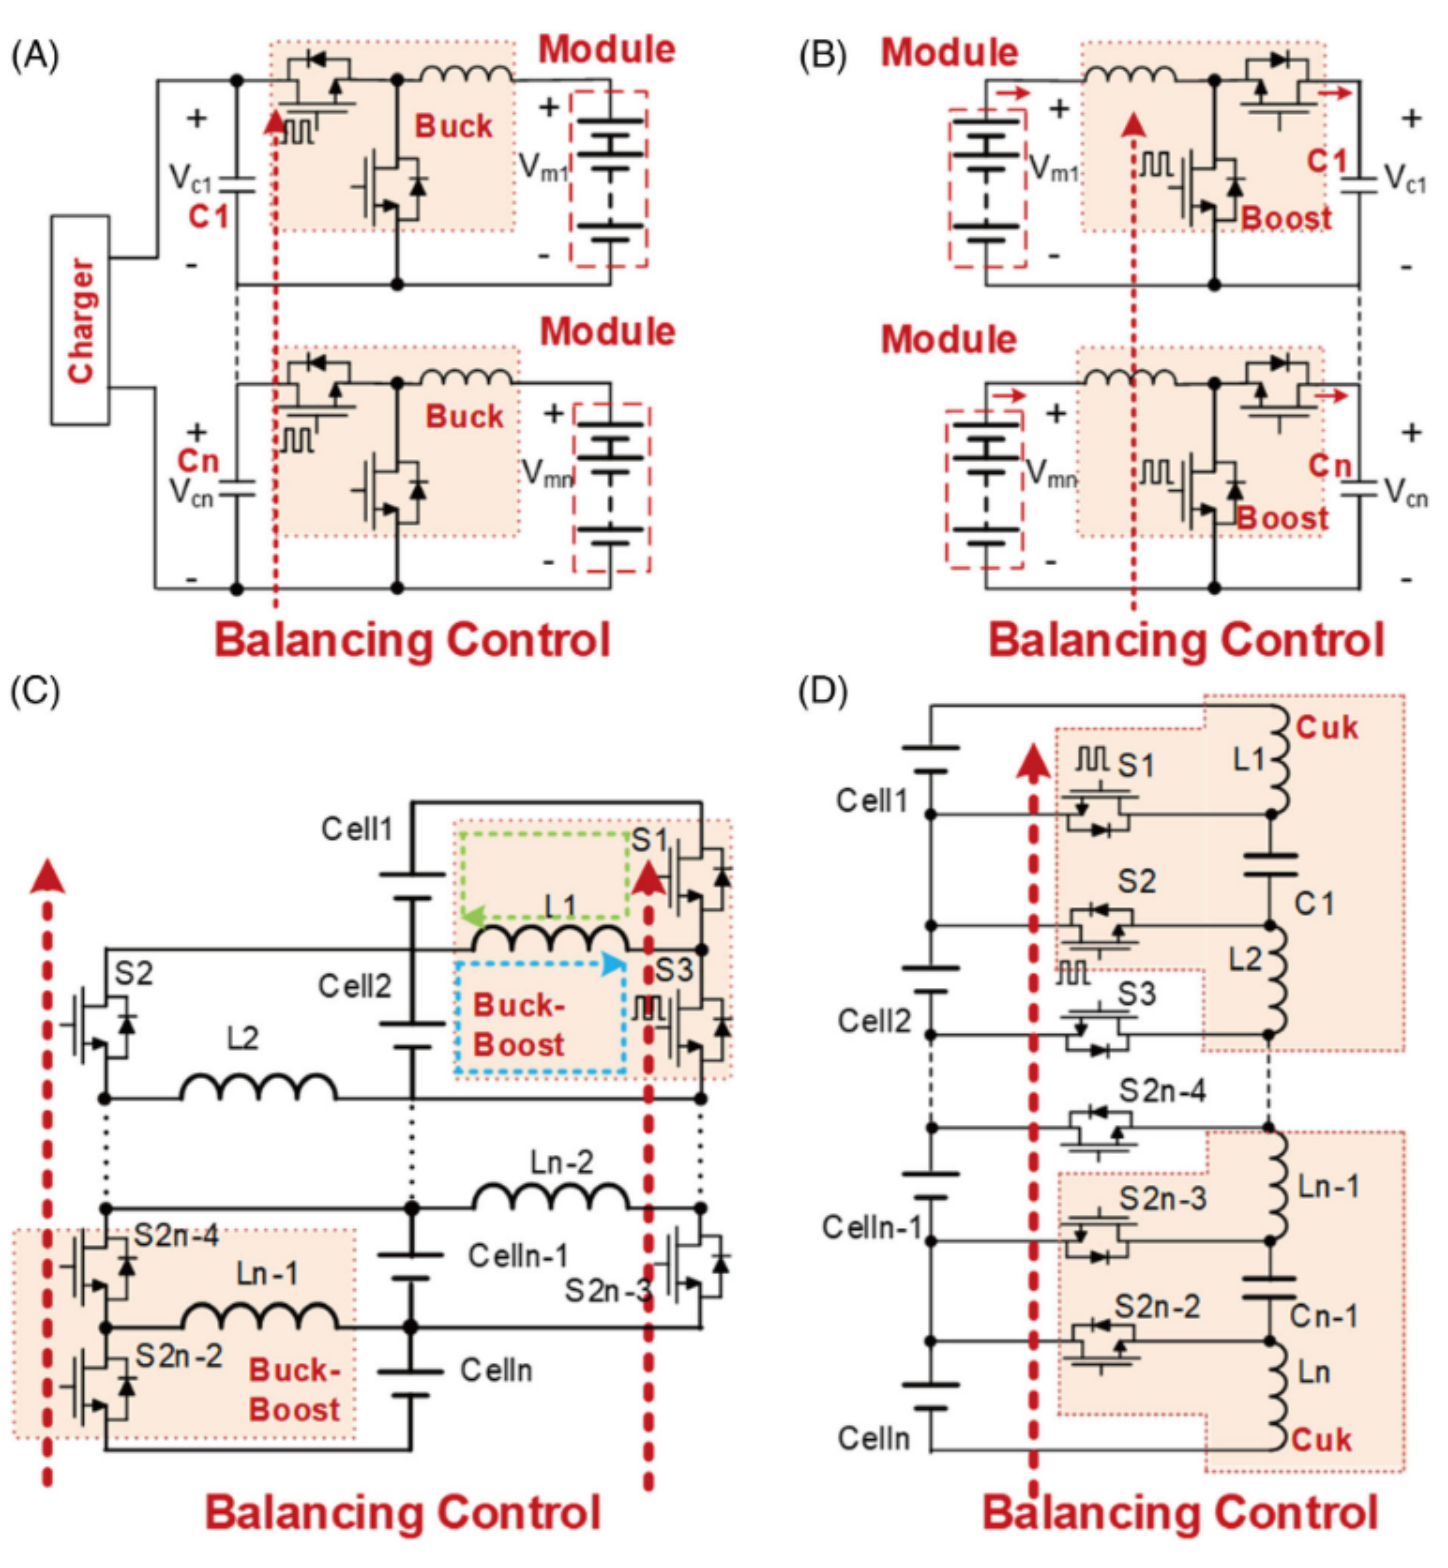
\includegraphics[width=0.8\textwidth]{pbbc_top.png}
        \caption{Topolog\'ias de balanceo basadas en convertidores de potencia.
                 (A) Topolog\'ia de ecualizaci\'on basadas en convertidores
                 reductores. (B) Topolog\'ia de ecualizaci\'on basadas en
                 convertidores elevadores. (C) Topolog\'ia de ecualizaci\'on
                 basada en una topolog\'ia reductor-elevador (\acrshort{C2C}).
                 (D) Topolog\'ia Cuk (\acrshort{C2C}).}
         \label{pbbc_top}
    \end{center}
\end{figure}
\FloatBarrier

%\newpage

\subsubsection{Topolog\'ias h\'ibridas}

Las topolog\'ias h\'ibridas pueden mejorar el rendimiento del balanceador
gracias a la combinaci\'on de una ecualizaci\'on pasiva con una activa. 
Los autores en \cite{fang_bal} proponen una topolog\'ia h\'ibrida basada en 
convertidores de potencia y resistencias \emph{shunt}. El convertidor de 
potencia puede transferir energ\'ia del m\'odulo para cargar las bater\'ias con 
un voltaje bajo, y las bater\'ias con mayor carga pueden ser descargadas a 
trav\'es de la resistencia \emph{shunt} conectadas en paralelo.

Los autores en \cite{zhang_et_al_hier} proponen una topolog\'ia de balanceo 
jer\'arquica para mejorar la ecualizaci\'on de celdas conectadas en serie, cuyo 
esquem\'atico se puede observar en la Figura \ref{hier_bal_top}. Esta 
topolog\'ia incluye dos capas de balanceo. La capa superior transfiere energ\'ia 
entre ambos m\'odulos basados en transformadores de m\'ultiplos devanados, y la 
capa inferior implementa convertidores de potencia reductor-elevador para 
transferir energ\'ia entre bater\'ias contiguas del mismo m\'odulo. De esta 
manera, esta topolog\'ia logra disminuir las corrientes de p\'erdida durante el 
proceso de balanceo.

\begin{figure}[h!]
    \begin{center}
        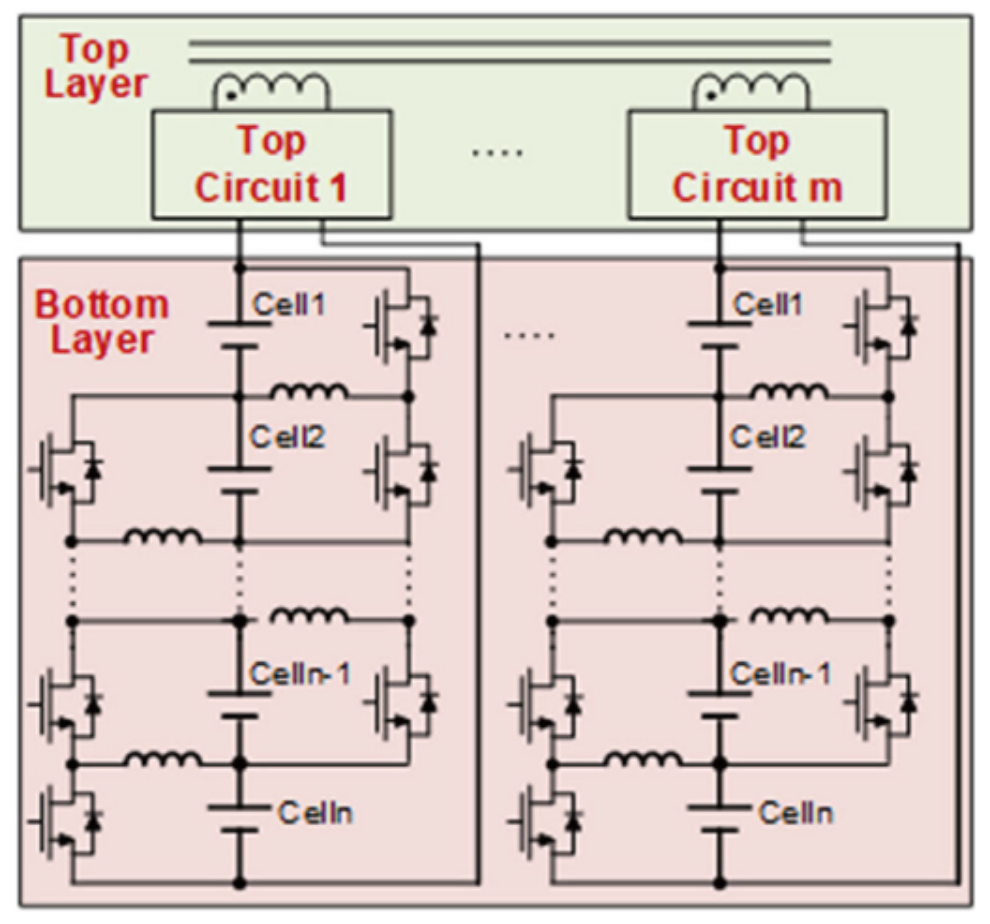
\includegraphics[width=0.6\textwidth]{hbbc_top.png}
        \caption{Topolog\'ia de balanceo jer\'arquica}
        \label{hier_bal_top}
    \end{center}
\end{figure}

\subsubsubsection{Comparaci\'on de topolog\'ias}

La topolog\'ia es el fundamento principal de los sistemas de ecualizaci\'on de
bater\'ias, la misma determina el costo y el tamaño del sistema completo. Una
topolog\'ia eficiente es esencial para extender el ciclo de vida de un pack de
bater\'ias y mejorar su rendimiento efectivamente. Es crucial seleccionar la
topolog\'ia adecuada seg\'un los requerimientos del sistema. 

Las topolog\'ias pasivas tienen las ventajas de ser circuitos simples, de bajo
costo y convenientes de implementar, por lo tanto, han sido ampliamente
adoptados por los \acrshort{VVEE}s. Sin embargo, esta clase de topolog\'ias
generalmente tienen tiempos de balanceo muy lentos y solo disipan energ\'ia
reduciendo la eficiencia del sistema.

Por el otro lado, la topolog\'ia activa es popular gracias a su buena eficiencia
y bajas p\'erdidas de potencia. Comparado con la ecualizaci\'on pasiva, la
topolog\'ia activa puede efectivamente reducir la inconsistencia entre las
capacidades entre celdas y resistencias internas mejorando el tiempo de vida del
pack de bater\'ias y su energ\'ia disponible.
%\newpage
Dentro de los sistemas de balanceo activo, los \acrshort{CBBC}s tienen el
m\'erito de implementar una estrategia muy simple y de bajo costo, con la
contraparte de que los tiempos de ecualizaci\'on son muy bajos. Los
\acrshort{IBBC}s puede transferir energ\'ia de forma bidireccional y tienen una
velocidad de balanceo moderada, pero tienen problemas de \acrshort{EMI} y una
estrategia de balanceo compleja de implementar. \acrshort{TBBC}s pueden proveer
altas corrientes de ecualizaci\'on, con la contraparte de que su manufactura es
compleja debido a la fabricaci\'on de transformadores con devanados
sim\'etricos. Por \'ultimo los \acrshort{PBBC}s tales como los
convertidores reductores-elevadores y Cuk son atractivos gracias a su alta
corriente de balanceo y su f\'acil integrac\'ion en el circuito, sin embargo,
estos resultan complejos y traen apareados estrategias de control complicadas.

Debido a que el esquema pasivo y activo tienen caracter\'isticas muy distintas
entre si, pueden ser aplicados en distintos escenarios seg\'un la aplicaci\'on
en cuesti\'on, por ejemplo, los esquemas pasivos pueden ser implementados en
\acrshort{VVEE}s de baja potencia o en veh\'iculos h\'ibridos mientras que las
topolog\'ias activas son generalmente implementadas en \acrshort{VVEE}s de alta
potencia.

El Cuadro \ref{comp_bal_table} condensa las ventajas y desventajas de cada
topolog\'ia y la Figura \ref{comp_bal_results} muestra un resultado de las
comparanciones entre ellas. 

\begin{table}[h!]
\begin{center}
\begin{tabular}{@{}llcccccc@{}}
\toprule
\multicolumn{2}{l}{Topologias de balanceo}                                                 & Tiempo & Estructura & Control & Eficiencia & Volumen & Costo \\ \midrule
\multirow{4}{*}{\acrshort{CBBC}} & Ecualizacion pasiva                    & 2      & 5                       & 5                     & 1          & 5       & 5     \\
                                                  & Capacitor alternativo                  & 2      & 4                       & 4                     & 4          & 4       & 4     \\
                                                  & Dos capas de capacitores               & 3      & 3                       & 3                     & 3          & 3       & 4     \\
                                                  & Multi-capas de capacitores             & 3      & 2                       & 2                     & 2          & 3       & 3     \\
\acrshort{IBBC}                  & Multiples inductores                   & 4      & 3                       & 3                     & 3          & 2       & 2     \\
\acrshort{TBBC}                  & Multiples devanados & 4      & 2                       & 3                     & 3          & 2       & 2     \\
\multirow{2}{*}{\acrshort{PBBC}} & Cuk                                    & 4      & 2                       & 2                     & 2          & 3       & 2     \\
                                                  & reductor-elevador                      & 4      & 2                       & 2                     & 2          & 3       & 2     \\ \cmidrule(l){2-8}
\end{tabular}
\caption{La clasificaci\'on est\'a puntuada del 1 al 5. Donde 1 es el peor
y 5 el mejor.}
\label{comp_bal_table}
\end{center}
\end{table}

\begin{figure}[h!]
    \begin{center}
        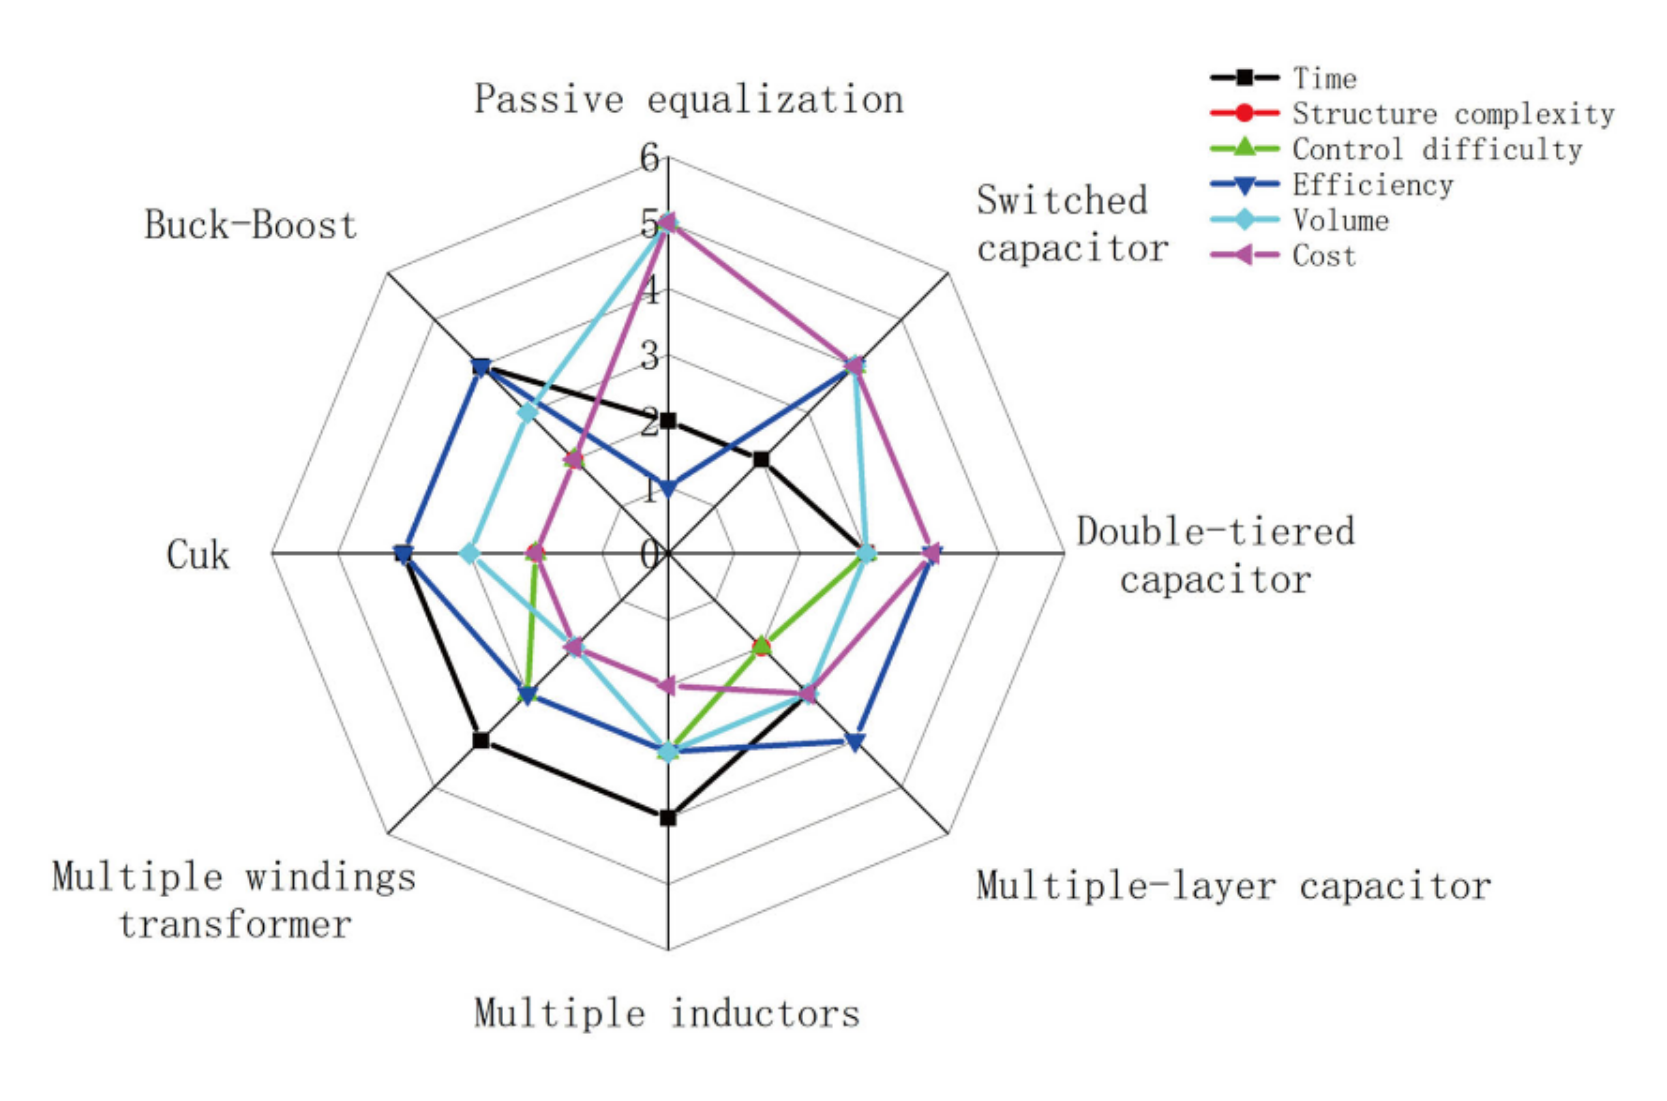
\includegraphics[width=0.8\textwidth]{comp_eq_chart.png}
        \caption{Gr\'afica comparativan de las distintas topolog\'ias disponibles}
        \label{comp_bal_results}
    \end{center}
\end{figure}
%\newpage
\subsubsection{Estrategias de ecualizaci\'on}

Las estrategias de ecualizaci\'on son utilizadas para controlar la operaci\'on
del balanceo teniendo un alto impacto sobre este proceso. Una estrategia de 
ecualizaci\'on inapropiadas para la ecualizaci\'on pueden llevar a problemas de 
desbalanceo o sobrebalanceo, resultando en p\'erdida de potencia innecesaria y 
decaimiento del pack de bater\'ias. Las variables a ecualizar y los algoritmos 
de control son los temas a tener en cuenta en las estrategias de ecualizaci\'on, 
y el desglose de las mismas se puede observar en la Figura 
\ref{eq_strategy_class}.

\begin{figure}[h!]
    \begin{center}
        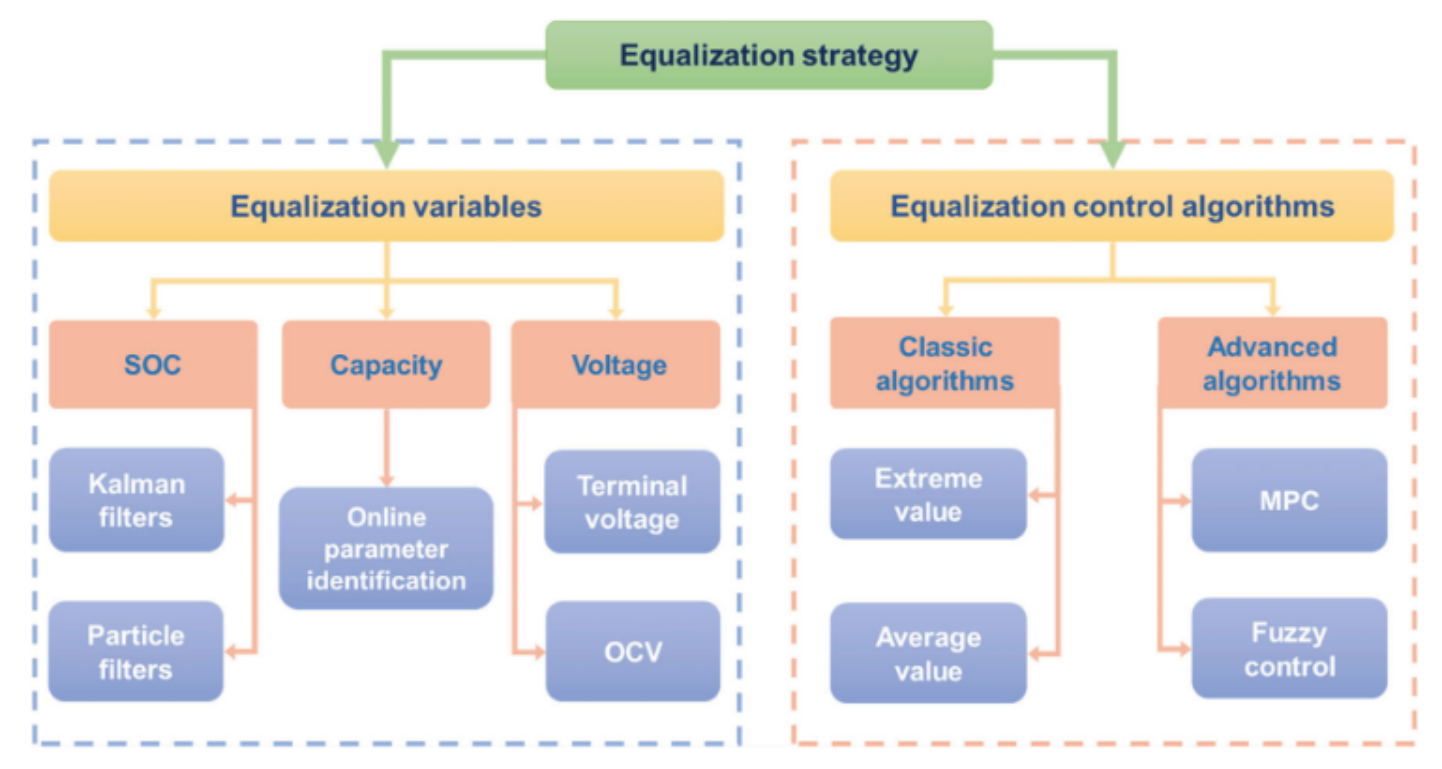
\includegraphics[width=.8\textwidth]{eq_strategy_class.png}
        \caption{Los perfiles de las estrateg\'as de ecualizaci\'on y sus
                 clasificaciones}
        \label{eq_strategy_class}
    \end{center}
\end{figure}

\subsubsubsection{Variables de Ecualizaci\'on}

Las variables de ecualizaci\'on son la base para las estrategias de
ecualizaci\'on. El error de la muestra, el costo computacional y el car\'acter de
hist\'eresis deben ser consideradas a la hora de elegir qué variable ecualizar.
Para la ecualizaci\'on se encuentran tres variables disponibles, el voltaje de 
las celdas, \acrshort{SOC}, capacidad y resistencia interna.

\subsubsubsection{Estrategias de Ecualizaci\'on basadas en voltaje
(\acrshort{VBES})}

Los \acrshort{VBES} (del ingl\'es, \acrlong{VBES}) usan el voltaje de las celdas
medidos en sus terminales por el \acrshort{BMS} como la base para seleccionar
qué bater\'ias deben ser ecualizada. La medición del voltaje en bornes de las
celdas conectadas en serie puede ser realizado de forma directa con una
exactitud aceptable, por lo tanto, los \acrshort{VBES}s son uno de los m\'etodos
viables m\'as b\'asicos a implementar. Sin embargo, las características no
lineales de las celdas de litio, cuestión que se desprende de la Sección
\ref{litioModel} y las particularidades que se presentan a la hora de modelar
una celda, nos permite inferir que el voltaje en bornes no refleja el valor real
\acrshort{OCV} causando dificultades a la hora de utilizar esta variable para
decidir sobre el proceso de ecualizaci\'on de las celdas.

Para subsanar este problema, se propone una estrategia de ecualizaci\'on basada
en el \acrshort{OCV}. Sin embargo, la medici\'on en tiempo real de esta variable
no es viable ya que se necesita un largo tiempo de descanso para que la celda
refleje esta variable en los terminales de la misma.

Debido a que la resistencia interna puede causar una ca\'ida de voltaje
inmediata cuando circula corriente sobre la celda, la diferencia de tensi\'on se
ve afectada a trav\'es de todas las celdas conectadas en serie ante un m\'inimo
est\'imulo sobre ellas. Por lo tanto, esta metodolog\'ia no funcionar\'a
adecuadamente salvo que el veh\'iculo est\'e completamente parado.
Generalmente, este tipo de estrategias son usadas con ternas de celdas de
litio-ion con una linealidad relativa en la curva \acrshort{OCV}-\acrshort{SOC},
pero no son efectivas y corren el riesgo de un desbalanceo cuando son utilizadas
en celdas tipo LiFeP$\mathrm{O_4}$. 

\subsubsubsection{Estrategias de Ecualizaci\'on basadas en la capacidad
(\acrshort{CBES})}

Las \acrshort{CBES} (del ing\'es, \emph{\acrlong{CBES}}) se basan en balancear
la capacidad actual de la bater\'ia. Sin embargo, la capacidad de las bater\'ias
se ven influenciadas por condiciones tales como la corriente y la temperatura
por lo que identificar su valor es complicado y lograr una uniformidad entre
celdas de un pack.

\subsubsubsection{Estrateg\'ia de Ecualizaci\'on basada en el \acrshort{SOC}}

Como se menciona en la secci\'on \ref{algSoc}, el \acrshort{SOC} es una variable
que permite caracterizar la capacidad remanente en una celda. La literatura
actual demuestra que la ecualizaci\'on basada en \acrshort{SOC} puede ser m\'as 
robusta que la basada en voltaje bajo condiciones din\'amicas de operaci\'on.
Sin embargo, el \acrshort{SOC} no puede ser medido de forma directa, si no que
tiene que ser estimado con cierta gravedad de error.

\subsubsubsection{Estrategia de Ecualizaci\'on basada en m\'etodos h\'ibridos}

Este tipo de m\'etodo consiste en tomar ventaja de varias estrategias de
ecualizaci\'on. Por ejemplo, en \cite{ZHANG20194702} se propone el desarrollo de 
un algoritmo h\'ibrido basado en el \acrshort{SOC} y el voltaje, y adopta 
estrategias correspondientes seg\'un distintos rangos de voltaje. Las 
simulaciones muestran resultados de balanceo m\'as eficientes que las basadas 
solamente en el \acrshort{SOC}. 

Por el otro lado, considerando la relaci\'on entre la inconsistencia con la
degradaci\'on de la bater\'ia, el \acrshort{SOC} y el \acrshort{SOH} pueden ser
combinados para obtener un mejor rendimiento de balanceo. Los autores en
\cite{REN2019908} presentan un sistema de ecualizaci\'on h\'ibrido que consiste 
en acoplar la estimaci\'on de ambas variables. Los resultados de las 
simulaciones realizadas demuestran que un m\'etodo de balanceo activo puede 
mejorar el desbalance del \acrshort{SOC} entre celdas.

\subsubsubsection{Comparaci\'on de las variables de control}

Como se menciona anteriormente, la variable a controlar para realizar la
ecualizaci\'on del pack de bater\'ias es crucial para lograr un balanceo
eficiente. La ecualizaci\'on basada en el voltaje de cada celda es el m\'etodo
m\'as f\'acil de implemetar ya que su medicion se puede realizar de forma
directa, sin embargo, lleva apareado una gran cantidad de inconvenientes, como
por ejemplo, la polarizaci\'on de la celda y el error de la medici\'on pueden
llevar a que el balanceo sea ineficiente poniendo en riesgo la salud del pack
de bater\'ias. Por el otro lado, las estrategias basadas en \acrshort{SOC} y
capacidad de la bater\'ia tienen el beneficio de poder determinar un desbalanceo
de forma m\'as eficiente pero bajo el costo de necesitar un sistema de
c\'omputos que permita estimar las variables bajo estudio. Finalmente, surgen
los m\'etodos h\'ibridos que se encargan de fusionar ambas variables, como el
voltaje y el \acrshort{SOC} para combinar ambas ventajas y obtener una
ecualizaci\'on m\'as robusta del sistema.

\subsubsection{Algoritmos de control para la ecualizaci\'on}

Los algoritmos de control son cruciales para el rendimiento de la
ecualizaci\'on, son utilizados para determinar el tiempo de balanceo y
corriente. Generalmente, estos algoritmos se pueden dividir en dos grupos:
algoritmos cl\'asicos de control (\acrshort{CCA}, del ingl\'es \acrlong{CCA}) y
algortimos avanzados de control (\acrshort{ACA}, del ingl\'es \acrlong{ACA}).
Estos algoritmos son posibles de implementar en determinados casos y deben ser
seleccionados acorde al costo computacional, intervalo de muestreo y el nivel de
robustez requerido.

\subsubsubsection{Algortimos cl\'asicos de control}

Los \acrshort{CCA}s realizan operaciones matem\'aticas basadas en las variables
de ecualizaci\'on selccionadas. Normalmente, los \acrshort{CCA}s utilizan el
resultado de operaciones aritm\'eticas cl\'asicas tales como el promedio,
desviaciones estandards y varianzas como los criterios de ecualizaci\'on. Debido
a las ventajas en flexibilidad de c\'alculo y f\'acil implementaci\'on estos
m\'etodos han sido adoptados en aplicaciones de \acrshort{VVEE}s en las
\'ultimas d\'ecadas.

El algoritmo de ecualizaci\'on basado en valores extremos (\acrshort{EVEA}, del
ingl\'es \emph{\acrlong{EVEA}}) aplica los extremos de la variable de ecualizaci\'on
como el objetivo de balanceo. Los \acrshort{EVEA}s son b\'asicos y efectivos con 
un costo computacional bastante limitado, sin embargo suelen tener problemas de
desbalanceo debido a que no son robustos en casos como en la que la diferencia
entre ambos extremos no es lo suficiente grande, el sistema puede llegar a
sobre-balancear el sistema y degradar el rendimiento de la bater\'ia.

El algoritmo de ecualizaci\'on basado en el valor promedio (\acrshort{AVAE}, del
ingl\'es \emph{\acrlong{AVAE}}) calcula el promedio de la variable de
ecualizaci\'on seleccionada y despu\'es utiliza el criterio del valor promedio
para implementar la l\'ogica de balanceo. Este tipo de algoritmo es usado
ampliamente en \acrshort{VVEE}s debido a que son simples y confiables. La
eficiencia de ecualizaci\'on y el tiempo de balanceo puede verse afectado por
las variables seleccionadas, que deben ser consideradas cuidadosamente basado en
condiciones espec\'ificas.

\subsubsubsection{Algoritmos de control avanzado}

Muchos de los m\'etodos avanzados de control, como por ejemplo el control
predictivo y el control por l\'ogica difusa fueron implementados en muchas
aplicaciones de ecualizaci\'on.

El control predictivo es un m\'etodo de la teor\'ia de control avanzada que usa
una optimizaci\'on m\'ovil en tiempo real para predecir los cambios din\'amicos
y ajustar el control acorde a estos cambios, logrando en todo punto de 
operaci\'on un \'optimo rendimiento en el balanceo. Comparado con los
algoritmos de optimizaci\'on, el control predictivo tiene menor costo
computacional y ha sido usado ampliamente en sistemas de control no lineales.
Este m\'etodo puede subsanar la no linealidad de las celdas de litio, ya que
pueden predecir el estado de la bater\'ia y el offset de polarizaci\'on.
Comparado con un control promedio de \acrshort{SOC}, el mismo puede converger a
\acrshort{SOC}s y voltajes m\'as uniformes evitando de esta forma cualquier tipo
de sobre-balanceo.

El control basado en l\'ogica difusa es otro control perteneciente a la teor\'ia
del control avanzado que procesa informaci\'on imprecisa que depende de un grado
de conocimiento del sistema. En \cite{jia_et_al_fuzzy} se propone un controlador 
de tipo fuzzy que utiliza como entrada el nivel de desbalanceo y la corriente de 
carga que circula por el pack de bater\'ias. Los resultados demuestran que este 
m\'etodo es robusto y puede ecualizar el sistema en un tiempo corto.

Por \'ultimo, en la literatura se propuso el uso de redes neuronales,
controladores tipo PID y algoritmos acoplados como potenciales algoritmos de
control para mejorar el rendimiento del balanceo.

\subsubsubsection{Comparaci\'on de algoritmos de control}

Los algoritmos basados en el control cl\'asico fueron las primeras
implementaciones de balanceo utilizadas en \acrshort{VVEE}s debido a sus 
ventajas en cuanto a la baja complejicidad de implementaci\'on. Sin embargo, 
\'estos son propensos a causar desbalanceos debido a factores relacionados al 
ruido y al error de muestreo asociado con el l\'imite computacional para 
sistemas embebidos en \acrshort{VVEE}s.

Adicionalmente, los algoritmos de control avanzado tambi\'en son ampliamente
utilizados en aplicaciones de almacenamiento de energ\'ia en celdas de
litio-ion. Son caracterizados por tener una r\'apida convergencia, estabilidad y
robustos, mejorando los problemas de sobre y desbalanceo de celdas. Sin embargo,
estos sistemas est\'an apareados a un alto costo computacional, y el rendimiento
del control depende exclusivamente de la precisi\'on del modelo, que es
complicado de obtener.

\subsection{Sensado de Corriente}

El sensado de la corriente de carga como de descarga del pack de batería juega
un rol muy importante en el desarrollo exitoso de un \acrshort{BMS}. Es a partir
de conocer con precisión la magnitud de corriente que el sistema podrá mantener
el pack de baterías operando dentro de la zona segura (\acrshort{SOA} por sus
siglas en ingles), monitorear la distribución de carga entre las celdas,
implementar correctamente los algoritmos de ecualización de carga y mantener un
seguimiento preciso del estado de carga.

\noindent Existen en el mercado una gran variedad de tecnologías y 
soluciones para la medición de corriente en las diferentes aplicaciones. 
Algunas de las tecnologías más relevantes, disponibles en el mercado son:
\begin{itemize}
    \item Resistencia Shunt
    \item Transformadores de intensidad (TI)
    \item Bobina de Rogowski 
    \item Sensores de Efecto Hall
    \item Sensores de Impedancia Magnética (MI)
    \item Sensores de Magnetoresistencia Gigante 
    \item Sensores Ópticos (Experimental)
\end{itemize}

Dentro del amplio abanico de métodos y tecnologías utilizadas para la medición
de corrientes los dos más elegidos e implementados en Sistemas de Administración
de Baterías \acrshort{BMS} son las mediciones a partir de resistencias Shunt y
mediciones a partir de sensores de efecto hall debido a las caracter\'isticas de
ambas metodolog\'ias.

\subsubsection{Resistencia Shunt}

La tecnología Shunt se vale del Sensado de la caída del voltaje sobre una
resistencia de unos pocos mili ohmios en serie con el paso de la corriente
incógnita para la medición indirecta de la corriente.

El método de sensado por resistencia tipo shunt presenta una de las mejores
relaciones costos-efectividad, presentando un empaquetado compacto y aplicable
en mediciones de corrientes tanto continua como alterna encontrando su
frecuencia de corte por encima de las decenas de Mhz.

Las mediciones por resistencia shunt carecen naturalmente de aislación galvánica
debiendo ser resuelta a partir del circuito de implementación. Generalmente, los
shunts presentan bajo coeficiente de temperatura de resistencia, (\acrfull{TCR}
por sus siglas en ingles). Característica fundamental en las implementaciones de
\acrshort{BMS} en sistemas de vehículos eléctricos que permite aumentar el rango
de temperatura de operación del sistema.

Aunque los shunts de corrientes operen bajo el principio de caida de voltaje
ohmico, en la práctica las resistencias presentan una inductancia intrínseca que
comprometen la precisión y el ancho de banda máximo de las mediciones.

\subsubsection{Sensor de efecto Hall}

El sensor de efecto Hall es un sensor de efecto magnético basado en el fenómeno
físico homónimo que le da su nombre.  El sensor de efecto Hall es un dispositivo
aislado, no intrusivo que puede ser utilizado para medir corriente tanto
continua como alterna de hasta unos cientos de kHz. El sensor Hall puede ser
fabricado utilizando tecnología CMOS convencional pero a un costo mayor que las
implementaciones con transformadores de corriente o bobinas de Rogowski.

El traductor de efecto Hall encuentra normalmente su límite de medición en los
picos de corriente debido al fenómeno de saturación magnética del núcleo y
encuentra su límite de ancho de banda en las frecuencias menores al MHz. A su
vez, esta tecnología es sumamente sensible a la influencia de los campos
magnéticos externos. Frente a estas limitaciones es común que los sensores de
efecto Hall se implementen mayoritariamente con bobinas cerradas para lograr una
mejor precisión y un rango mayor de operación dinámico.

El voltaje de offset presente en la medición del dispositivo es poco estable y
varia fuertemente frente a las variaciones de temperatura de operación.

\begin{figure}[h!]
    \centering
    \begin{subfigure}[b]{0.4\linewidth}
	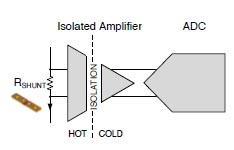
\includegraphics[width=\linewidth]{../assets/R-Shunt_Isolated_Sensor.jpg}
	\caption{Sensado por Resistencia Shunt}
    \end{subfigure}%
    \hspace{15mm}
    \begin{subfigure}[b]{0.4\linewidth}
	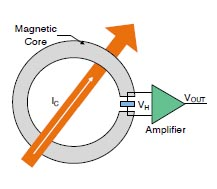
\includegraphics[width=\linewidth]{../assets/Open-loop_Hall_Sensor.jpg}
	\caption{Sensado por efecto Hall de loop abierto}
    \end{subfigure}
    \caption{Diagramas - Métodos de sensado de corriente}
    \label{fig:SenseMetods}
\end{figure}

\newpage

\subsection{Protocolos de comunicación}
En la actualidad es innegable la expansión de la tecnología y la electrónica haciendose más presentes en nuestro día a día, hoy no es raro escuchar de domótica, IoT y Smart Devices.Los vehículos no son la excepción y aún en los vehículos de 4 plazas de gamma baja se integran un conjunto de sensores, actuadores y controladores electrónicos.
Estos dispositivos se hayan interconectados entre sí por redes de comunicación transmitiendo señales en tiempo real y recabando información y controlando los diversos procesos que ocurren permanentemente en el vehiculo. Así como también reportando fallas al usuario permitiendo tomar deciciones anticipadas, facilitando el mantenimiento de la unidad.

En los vehiculos actuales los protocolos más utilizados en los vehículos son \acrshort{CAN}, por sus siglas en inglés \acrfull{CAN},  (tanto de alta como de baja velocidad), \acrshort{LIN} del inglés, \acrfull{LIN} y \acrshort{MOST} del inglés, \acrfull{MOST} \cite{Vela2016}.

Dentro del vehículo hallamos sistemas de naturaleza muy variada, por ejemplo, el sistema de frenos ABS, el cierre centralizado, las luces de interior y el canal de audio del sistema de sonido. Cada uno de los cuales tiene requerimientos totalmente distintos, en el caso del sistema ABS los tiempos de reacción deben ser del orden del milisegundo pero con un volumen de datos mínimo, mientras que por el contrario el sistema de sonido tiene un volumen de datos mucho mayor con una prioridad mucho menor ya que es un sistema de entretenimiento y no de seguridad.

De los protocolos mencionados el más utilizado por su superadora relación costo-confiabilidad es el protocolo \acrshort{CAN}, debido a la arquitectura multiplexada con un único bus serie que reduce costos combinada con algoritmos de detección de errores que brindan confiabilidad a la red. Otra de las ventajas de CAN es que si un dispositivo sale de servicio la red continua funcionando perfectamente, además de contar con control de acceso al medio con prioridad. Todo esto hace de CAN un protocolo que desde sus orígenes es óptimo para el rubro automotríz.

\subsubsection{Protocolo CAN}
Este es un protocolo desarrollado inicialmente por la empresa alemana Robert Bosch GmbH en 1983 la cual fue aceptada ampliamente y que posterior mente fue definida como estándar que en su especificación ISO 11898 describe como la información será transmitida entre los diferentes dispositivos de red.

Las principales características de este protocolo son \cite{RBG1991}:
\begin{itemize}
	\item Priorización de mensajes
	\item Sistema Multi-Maestro
	\item Configuración Flexible
	\item Velocidad de transmisión media (hasta 1 Mbit/s)
	\item Señalización y detección de fallas.
\end{itemize}

Para  detectar  errores  a  nivel  de  mensajes  el  protocolo  implementa  tres  
mecanismos: chequeo de redundancia cíclica (CRC), chequeo de formato de trama y 
acuse de recibo (ACK).

Para detectar errores a nivel de bit el protocolo implementa dos mecanismos: 

\begin{itemize}
	\item Monitoreo. Cada nodo transmisor monitorea el nivel del bus a fin 
de detectar la diferencia entre el bit enviado y el recibido. 
	\item Bits de Relleno (Bit stuffing). CAN utiliza la codificación NRZ (no 
retorno a cero) y la técnica de bit  stuffing,  que consiste en insertar un bit complementario cada cinco bits iguales consecutivos transmitidos. 
\end{itemize}

Trabaja en según el modelo \acrshort{OSI} (\acrfull{OSI}) en la primera y la segunda capa, también conocidas como la capa física y la capa de enlace de datos respectivamente.

El protocolo CAN  sólo define las dos primeras capas del Modelo \acrshort{OSI} (\acrfull{OSI}) (física y enlace), aunque no especifica la interfaz al medio físico (Medio de transmisión, conectores).La norma ISO 11898 es el estándar internacional para la comunicación de alta velocidad usando el protocolo de bus CAN. Esencialmente este estándar define las capas física y de enlace de datos.

\subsubsubsection{Capa Física} 
La capa física en \acrshort{CAN} es responsable de la transferencia de bits entre los distintos nodos que componen la red. Define aspectos como, niveles de señal, codificación, sincronización y tiempos en que los bits se transfieren al bus.
En la especificación original de \acrshort{CAN}, la capa física no fue definida, permitiendo diferentes opciones para la elección del medio y niveles eléctrico de transmisión. Las características de las señales eléctricas en el bus fueron establecidas más tarde por el estandar ISO 11898.

La especificación \acrfull{CiA}, complementó las definiciones respecto al medio físico y conectores. Los nodos conectados al bus interpretan dos niveles lógicos denominados:

\begin{itemize}
	
	\item Dominante: La tensión diferencial (CAN-H - CAN-L) es del orden de 2.0V con CAN-H = 3.5V y CAN-L = 1.5V (nominales).\\
	\item Recesivo: La tensión diferencial (CAN-H - CAN-L) es del orden de 0V con CAN-H = 2.5V y CAN-L = 2.5V (nominales).\\
	
\end{itemize}

La topología es bus con derivaciones de corta longitud.Si se presenta el caso de perdida de prestaciones en cuanto a velocidad o longitud máxima se pueden adoptar topologias en estrella. El bus se cierra en los extremos con impedancias de carga.

El número máximo de nodos no está limitado por la especificación básica y depende de las características de los transreceptores, las especificaciones de buses de campo lo limitan a 32 o 64 en una red sin repetidores.


\subsubsubsection{Capa de Datos}
Unas de las características que distingue a CAN con respecto a otras normas, es su técnica de acceso al medio denominada como 
CSMA/CD+CR o ``Carrier Sense, Multiple Access/Colission Detection + Collision Resolution" (Acceso múltiple con detección de 
portadora, detección de colisión más resolución de colisión). 

El  acceso  al  medio  por  medio  de  técnicas de acceso múltiple y detección de colisión evolucionaron desde el método ALOHA 
inicial  hasta  su  consagración  como  método  de  acceso  al  medio  de  las  redes  Ethernet,  con  técnica  CSMA/CD.    El  método  de  
acceso  al  medio  utilizado  en  bus  CAN  añade  una  característica  adicional:  la  resolución  de  colisión.    En  la  técnica  CSMA/CD  
utilizada en redes Ethernet ante colisión de varias tramas, todas se pierden, CAN resuelve la colisión con la supervivencia de una 
de  las  tramas  que  chocan  en  el  bus.    Además  la  trama  superviviente  es  aquella  a  la  que  se  ha  identificado  como  de  mayor  
prioridad. 

La resolución de colisión se basa en una topología eléctrica que aplica una función lógica determinista a cada bit, que se resuelve 
con la prioridad del nivel definido como bit de tipo dominante.  Definiendo el bit dominante como equivalente al valor lógico '0' y 
bit   recesivo  al   nivel  lógico  '1'  se  trata  de  una  función  AND  de  todos  los  bits  transmitidos  simultáneamente.    Cada  transmisor  
escucha  continuamente  el  valor  presente  en  el  bus,  y  se  retira  cuando  ese  valor  no  coincide  con  el  que  dicho  transmisor  ha  
forzado.    Mientras  hay  coincidencia  la  transmisión  continua,  finalmente  el  mensaje  con  identificador  de  máxima  prioridad  
sobrevive.  Los demás nodos reintentarán la transmisión lo antes posible.\\

\subsubsubsection{Mensajes y Tipos de Tramas}
CAN utiliza mensajes de estructura predefinida, tramas, para la gestión de la comunicación.
Se distinguen entre dos variantes de CAN, el definido en CAN 2.A o ``CAN Standard" y el definido en CAN 2.B o ``CAN
Extendido", los formatos de trama son análogos diferenciándose básicamente en el número de bits que se utiliza para el
identificador de mensaje: 11 bits (2032 identificadores) diferentes en CAN Standard y 29 bits (536.870.912 identificadores) en
CAN Extendido.
Las tramas CAN son de longitud reducida, la trama más larga es de 130 bits en CAN Estándar y 154 bits en CAN Extendido.
Los tipos de trama, y estados de bus, utilizados segun \cite{KaschelHector2004} son:
\begin{itemize}
	\item Trama de datos: la que un nodo utiliza normalmente para poner información en el bus (siempre es un ``broadcast" a todos los demás nodos). Puede incluir entre 0 y 8 Bytes de información útil.\\
	\item Trama de interrogación remota (en lo que sigue se denominará como trama remota (``remote frame"): puede ser utilizada por
	un nodo para solicitar la transmisión de una trama de datos con la información asociada a un identificador dado. El nodo que
	disponga de la información definida por el identificador la transmitirá en una trama de datos.\\
	\item Tramas de error: usadas para señalar al resto de nodos la detección de un error, invalidando el mensaje erróneo normalmente (un caso especial es un nodo en estado de ``error pasivo").\\
	\item Trama de sobrecarga: permite que un nodo fuerce a los demás a alargar el tiempo entre transmisión de tramas sucesivas
	Espaciado inter-tramas: Las tramas de datos (y de interrogación remota) se separan entre sí por una secuencia predefinida que
	se denomina espaciado inter-trama.\\
	\item Bus en reposo: En los intervalos de inactividad se mantiene constantemente el nivel recesivo del bus.\\
	\end{itemize}


\begin{comment}

En un bus CAN los nodos transmiten la información espontáneamente con tramas de datos, bien sea por un proceso cíclico o activado ante eventos en el nodo. La trama de interrogación remota sólo se suele utilizar para detección de presencia de nodos o para puesta al día de información en un nodo recién incorporado a la red. Los mensajes pueden entrar en colisión en el bus, el de identificador de mayor prioridad sobrevivirá y los demás son retransmitidos lo antes posible.



\subsubsubsection{Formatos de Trama}

	\textbf{Trama de Datos}\\
	Una trama de datos es generada por un nodo CAN cuando transmite información. Los campos incluidos en una trama de datos
	son para CAN Estándar.
	
	\begin{itemize}
	\item \textbf{Inicio de trama (SOF):} El inicio de trama es un campo de un solo bit siempre dominante que indica el inicio de la transmisión. Los nodos receptores se sincronizan con el flanco de bajada de este bit.\\
	\item \textbf{Arbitraje:} El campo de identificación está formado por el identificador de mensaje (11 bits) más el bit RTR. En una trama de datos el bit RTR es dominante. En una trama remota es recesivo. Los bits de identificador se transmiten en orden de más significativo a menos significativo.\\
	\item \textbf{Control:} El campo de control está formado por dos bits reservados para uso futuro y cuatro bits adicionales que indican el número de bytes de datos. En realidad el primero de estos bits (IDE) se utiliza para indicar si la trama es de CAN Estándar (IDE dominante) o Extendido (IDE recesivo). El segundo bit (RB0) es siempre recesivo. Los cuatro bits de código de longitud (DLC) indican en binario el número de bytes de datos en el mensaje (0 a 8).\\
	\item \textbf{Datos:} Es un campo formado por 0 a 8 bytes de datos, es decir 0 a 64 bits en saltos de 8. Cada byte se transmite con bit más significativo primero.\\
	\item \textbf{CRC:} Código de redundancia cíclica que genera el transmisor por la división módulo 2 de todos los bits precedentes del mensaje, incluyendo los de relleno si existen, por el polinomio generador: X15+ X14+ X8+ X7+ X4+ X3+ X1+1, el resto de esta división es el código CRC transmitido. Los receptores comprueban este código. Tras el código CRC se incluye un bit recesivo (delimitador de CRC).\\
	\item \textbf{Campo de reconocimiento (ACK):} es un campo de dos bits que el transmisor pone como recesivos. El primero de estos bits se
	sobreescribe por un bit dominante de reconocimiento transmitido por los nodos que han recibido el mensaje correctamente. El bit
	de ACK queda así insertado entre dos bits dominantes de delimitación.
	\item \textbf{Fin de trama (EOF)}: Cierra la trama, consiste en 7 bits recesivos sucesivos.\\
	\item \textbf{Espaciado entre tramas (IFS)}. Consta de un mínimo de 3 bits recesivos.\\
\end{itemize}

La trama de datos de CAN Extendido se diferencia de la de CAN Estándar en que un bit dominante fijo (SRR) aparece en la posición del bit RTR de CAN Estándar, se fija el bit IDE como recesivo, siguen luego los 18 bits adicionales del identificador, el campo de control con RTR, dos bits reservados y la longitud de datos y el resto de la trama es análogo.\\

En un bus CAN pueden convivir nodos CAN Estándar y CAN Extendido, para ello los nodos CAN Estándar han de ser del tipo CAN 2.OB Pasivo, estos nodos reaccionan ignorando tramas CAN Extendido en lugar de señalarlas como erróneas. Los nodos que cumplen CAN 2.0B pueden funcionar en modo Estándar o Extendido indistintamente.
Durante este trabajo se hará referencia sobre todo a CAN Estándar, en todo caso las diferencias con CAN Extendido son mínimas,
excepto la posibilidad de contar con un número mucho mayor de identificadores disponibles.\\

\textbf{Trama remota}\\

El formato es análogo a la trama de datos pero con el bit RTR recesivo . Por otra parte una trama remota no incluye nunca datos.
El identificador es el del mensaje que se solicita, el campo longitud corresponde a la longitud de ese mensaje.\\

\textbf{Trama de error}\\

Las tramas de error son generadas por cualquier nodo que detecta un error. Consiste en dos campos: Indicador de error (``Error
Flag") y Delimitador de error. El delimitador de error consta de 8 bits recesivos consecutivos y permite a los nodos reiniciar la
comunicación limpiamente tras el error. El Indicador de error es distinto según el estado de error (los estados de error de nodo se
describirán en páginas sucesivas) del nodo que detecta el error:
Si un nodo en estado de error ``Activo" detecta un error en el bus interrumpe la comunicación del mensaje en proceso generando
un "Indicador de error activo" que consiste en una secuencia de 6 bits dominantes sucesivos. Esta secuencia rompe la regla de
relleno de bits y provocará la generación de tramas de error en otros nodos. Por tanto el Indicador de error puede extenderse entre
6 y 12 bits dominantes sucesivos. Finalmente se espera el campo de delimitación de error formado por los 8 bits recesivos.
Entonces la comunicación se reinicia y el nodo que había sido interrumpido reintenta la transmisión del mensaje.
Si un nodo en estado de error ``Pasivo" detecta un error, el nodo transmite un ``Indicador de error pasivo" seguido, de nuevo, por el
campo delimitador de error. El indicador de error de tipo pasivo consiste en 6 bits recesivos seguidos y, por tanto, la trama de
error para un nodo pasivo es una secuencia de 14 bits recesivos. De aquí se deduce que la transmisión de una trama de error de ti
o pasivo no afectará a ningún nodo en la red, excepto cuando el error es detectado por el propio nodo que está transmitiendo. En
ese caso los demás nodos detectarán una violación de las reglas de relleno y transmitirán a su vez tramas de error.
Tras señalar un error por medio de la trama de error apropiada cada nodo transmite bits recesivos hasta que recibe un bit también
recesivo, luego transmite 7 bits recesivos consecutivos antes de finalizar el tratamiento de error.\\

\textbf{Espacio entre tramas}\\

El espacio entre tramas separa una trama (de cualquier tipo) de la siguiente trama de datos o interrogación remota. El espacio
entre tramas ha de constar de, al menos, 3 bits recesivos. Esta secuencia de bits se denomina ``íntermission". Una vez transcurrida
esta secuencia un nodo en estado de error activo puede iniciar una nueva transmisión o el bus permanecerá en reposo. Para un
nodo en estado error pasivo la situación es diferente, deberá espera una secuencia adicional de 8 bits recesivos antes de poder
iniciar una transmisión. De esta forma se asegura una ventaja en inicio de transmisión a los nodos en estado activo frente a los
nodos en estado pasivo.\\

\textbf{Trama de sobrecarga}\\

Una trama de sobrecarga tiene el mismo formato que una trama de error activo. Sin embargo, la trama de sobrecarga sólo puede
generarse durante el espacio entre tramas. De esta forma se diferencia de una trama de error, que sólo puede ser transmitida
durante la transmisión de un mensaje. La trama de sobrecarga consta de dos campos, el Indicador de Sobrecarga, y el delimitador.
El indicador de sobrecarga consta de 6 bits dominantes que pueden ser seguidos por los generados por otros nodos, dando lugar a
un máximo de 12 bits dominantes. El delimitador es de 8 bits recesivos.
Una trama de sobrecarga puede ser generada por cualquier nodo que debido a sus condiciones internas no está en condiciones de
iniciar la recepción de un nuevo mensaje. De esta forma retrasa el inicio de transmisión de un nuevo mensaje. Un nodo puede
generar como máximo 2 tramas de sobrecarga consecutivas para retrasar un mensaje. Otra razón para iniciar la transmisión de
una trama de sobrecarga es la detección por cualquier nodo de un bit dominante en los 3 bits de "intermission". Por todo ello una
trama de sobrecarga de generada por un nodo dará normalmente lugar a la generación de tramas de sobrecarga por los demás
nodos dando lugar, como se ha indicado, a un máximo de 12 bits dominantes de indicador de sobrecarga.\\

\textbf{Arbitraje}\\

Cada nodo que transmite, a su vez está monitoreando el dato que se refleja en el bus y se contrasta con el dato enviado por el mismo, en caso de no coincidir esto quiere decir que el transmisor de mayor prioridad es él mismo y continua la transmisión, de lo contrario detectará que hay un mensaje de mayor prioridad en el bus y lo leerá.

\end{comment}




